%\documentclass[AER]{AEA}
\documentclass[12pt,twoside]{report}
%\documentclass[12pt]{article}
%\documentclass[12pt,a4paper]{article}
\usepackage[english]{babel}

\usepackage[utf8]{inputenc}
\usepackage[T1]{fontenc}

\usepackage{mathtools,amsmath,amssymb,amsthm,amsfonts,mathrsfs}
\usepackage{booktabs,xtab,tabularx} %tabs
%\usepackage[lofdepth,lotdepth]
%\usepackage{subfig} 
\usepackage{authblk}
\usepackage{lscape}
\usepackage[outline]{contour}
\usepackage{qtree}
\usepackage{lmodern}
\usepackage{lipsum}
\usepackage{psl-cover} %%%%%%%%%%%%%%%%%%%%%%%%%%%%%%
%\usepackage[colorlinks=true,linkcolor=blue]{hyperref}
\usepackage[pdftex]{hyperref}
\usepackage{textcomp}
\usepackage{titlesec}
\usepackage[nottoc]{tocbibind}
\usepackage{titletoc,minitoc}
\usepackage{indentfirst}
\usepackage{afterpage}
\usepackage{tikz}
\tikzstyle arrowstyle=[scale=1]
\usetikzlibrary{spy,arrows,positioning,shapes.multipart}
\usetikzlibrary{shapes}
\usepackage{float}
%\usepackage[cmbold]{mathtime} %\usepackage{mt11p}
\usepackage{placeins}
\usepackage{caption}
\usepackage{color}
\usepackage{subfigure}
\usepackage{multirow,array}
\usepackage{epsfig}
\usepackage{listings}
\usepackage{enumitem}
\usepackage{rotating}
\usepackage{graphicx,graphics} %\usepackage[graphicx]{realboxes}
\usepackage{epstopdf,pdflscape}
\usepackage{longtable}
%\usepackage{breakurl}
\usepackage{epigraph}
\usepackage{xspace}
\usepackage{eurosym}
\usepackage{ulem}
\usepackage{verbatim}
\usepackage{footmisc}
\usepackage{comment}
\usepackage{setspace}
\usepackage{geometry}
\usepackage[authoryear]{natbib}
\usepackage{dcolumn}
%\usepackage[justification=centering]{caption}
%\captionsetup[table]{format=plain,labelformat=simple,labelsep=period,singlelinecheck=true}%
\bibliographystyle{apalike}
%\bibliographystyle{unsrtnat}
%\bibliographystyle{aea}
\usepackage{fancyhdr}
\pagestyle{fancy}


\def\checkmark{\tikz\fill[scale=0.4](0,.35) -- (.25,0) -- (1,.7) -- (.25,.15) -- cycle;}
%\usepackage{tikz}
%\usetikzlibrary{snakes}
%\usetikzlibrary{patterns}

%\draftSpacing{1.5}

\usepackage{xcolor}
\hypersetup{
colorlinks,
linkcolor={blue!50!black},
citecolor={blue!50!black},
urlcolor={blue!50!black}}

%\renewcommand{\familydefault}{\sfdefault}
%\usepackage{helvet}
%\setlength{\parindent}{0.4cm}
%\setlength{\parindent}{2em}
%\setlength{\parskip}{1em}

%\normalem

%\doublespacing
\onehalfspacing
%\singlespacing
%\linespread{1.5}

\newtheorem{theorem}{Theorem}
\newtheorem{corollary}[theorem]{Corollary}
\newtheorem{proposition}{Proposition}
\newtheorem{definition}{Definition}
\newtheorem{axiom}{Axiom}
\newtheorem{observation}{Observation}
\newtheorem{assumption}{Assumption}	
\newtheorem{remark}{Remark}
\newtheorem{lemma}{Lemma}
\newtheorem{result}{result}


\newcommand{\ra}[1]{\renewcommand{\arraystretch}{#1}}

\newcommand{\E}{\mathrm{E}}
\newcommand{\Var}{\mathrm{Var}}
\newcommand{\Corr}{\mathrm{Corr}}
\newcommand{\Cov}{\mathrm{Cov}}

\newcolumntype{d}[1]{D{.}{.}{#1}} % "decimal" column type
\renewcommand{\ast}{{}^{\textstyle *}} % for raised "asterisks"

\newtheorem{hyp}{Hypothesis}
\newtheorem{subhyp}{Hypothesis}[hyp]
\renewcommand{\thesubhyp}{\thehyp\alph{subhyp}}

\newcommand{\red}[1]{{\color{red} #1}}
\newcommand{\blue}[1]{{\color{blue} #1}}

%\newcommand*{\qed}{\hfill\ensuremath{\blacksquare}}%

\newcolumntype{L}[1]{>{\raggedright\let\newline\\arraybackslash\hspace{0pt}}m{#1}}
\newcolumntype{C}[1]{>{\centering\let\newline\\arraybackslash\hspace{0pt}}m{#1}}
\newcolumntype{R}[1]{>{\raggedleft\let\newline\\arraybackslash\hspace{0pt}}m{#1}}

%\geometry{left=1.5in,right=1.5in,top=1.5in,bottom=1.5in}
\geometry{a4paper,width=150mm,top=25mm,bottom=25mm,bindingoffset=6mm}


\epstopdfsetup{outdir=./}

\newcommand{\elabel}[1]{\label{eq:#1}}
\newcommand{\eref}[1]{Eq.~(\ref{eq:#1})}
\newcommand{\ceref}[2]{(\ref{eq:#1}#2)}
\newcommand{\Eref}[1]{Equation~(\ref{eq:#1})}
\newcommand{\erefs}[2]{Eqs.~(\ref{eq:#1}--\ref{eq:#2})}

\newcommand{\Sref}[1]{Section~\ref{sec:#1}}
\newcommand{\sref}[1]{Sec.~\ref{sec:#1}}

\newcommand{\Pref}[1]{Proposition~\ref{prop:#1}}
\newcommand{\pref}[1]{Prop.~\ref{prop:#1}}
\newcommand{\preflong}[1]{proposition~\ref{prop:#1}}

\newcommand{\Aref}[1]{Axiom~\ref{ax:#1}}

\newcommand{\clabel}[1]{\label{coro:#1}}
\newcommand{\Cref}[1]{Corollary~\ref{coro:#1}}
\newcommand{\cref}[1]{Cor.~\ref{coro:#1}}
\newcommand{\creflong}[1]{corollary~\ref{coro:#1}}

\newcommand{\etal}{{\it et~al.}\xspace}
\newcommand{\ie}{{\it i.e.}\ }
\newcommand{\eg}{{\it e.g.}\ }
\newcommand{\etc}{{\it etc.}\ }
\newcommand{\cf}{{\it c.f.}\ }
\newcommand{\ave}[1]{\left\langle#1 \right\rangle}
\newcommand{\person}[1]{{\it \sc #1}}

\newcommand{\AAA}[1]{\red{{\it AA: #1 AA}}}
\newcommand{\YB}[1]{\blue{{\it YB: #1 YB}}}

\newcommand{\flabel}[1]{\label{fig:#1}}
\newcommand{\fref}[1]{Fig.~\ref{fig:#1}}
\newcommand{\Fref}[1]{Figure~\ref{fig:#1}}

\newcommand{\tlabel}[1]{\label{tab:#1}}
\newcommand{\tref}[1]{Tab.~\ref{tab:#1}}
\newcommand{\Tref}[1]{Table~\ref{tab:#1}}

\newcommand{\be}{\begin{equation}}
\newcommand{\ee}{\end{equation}}
\newcommand{\bea}{\begin{eqnarray}}
\newcommand{\eea}{\end{eqnarray}}

\newcommand{\bi}{\begin{itemize}}
\newcommand{\ei}{\end{itemize}}

\newcommand{\Dt}{\Delta t}
\newcommand{\Dx}{\Delta x}
\newcommand{\Epsilon}{\mathcal{E}}
\newcommand{\etau}{\tau^\text{eqm}}
\newcommand{\wtau}{\widetilde{\tau}}
\newcommand{\xN}{\ave{x}_N}
\newcommand{\Sdata}{S^{\text{data}}}
\newcommand{\Smodel}{S^{\text{model}}}

\newcommand{\del}{D}
\newcommand{\hor}{H}

\def\firstcircle{(0,0) circle (4cm)}
\def\secondcircle{(60:2cm) circle (2cm)}
\def\thirdcircle{(30:2cm) circle (.9cm)}

\setlength{\parindent}{0.0cm}
\setlength{\parskip}{0.4em}

\numberwithin{equation}{section}
\DeclareMathOperator\erf{erf}
%\let\endtitlepage\relax

% First, we define three circles:
\def\firstcircle{(-0,0) circle (4)}
\def\secondcircle{(-1.6,1) circle (2)}
\pgfmathparse{-(2.4^2-2^2)^0.5} % by pythagoras
\let\h\pgfmathresult % shortcut for further use
\def\thirdcircle{(1,1) circle (1.5)}

\title{Innovation and choice}
\author{Diomides Mavroyiannis}
\date{\today}
\institute{Université Paris-Dauphine}
\doctoralschool{École doctorale de Dauphine}{543}
\specialty{Sciences économiques}

\jurymember{1}{M Jacques CHARMES}{CEPED-IRD}{Rapporteur}
\jurymember{2}{M Jean-François JACQUES}{Université Paris-Est Marne-la-Vallée}{Rapporteur}
\jurymember{3}{Mme Rym AYADI}{CASS Business School}{Examinateur}
\jurymember{4}{M Jérôme MATHIS}{Université Paris-Dauphine}{Examinateur}
\jurymember{5}{M Mouhoud EL-MOUHOUB}{Université Paris-Dauphine}{Examinateur}
\jurymember{6}{Mme Najat EL-MEKKAOUI}{Université Paris-Dauphine}{Directice de thèse}

\fancyhead[LE]{\textbf{\thepage}}
\fancyhead[LO]{\leftmark}
\fancyhead[RE]{\leftmark}
\fancyhead[RO]{\textbf{\thepage}}
\fancyfoot[C]{} 
\fancyfoot[L]{}
\fancyfoot[R]{}
\makeatletter

\newcommand{\thechaptername}{}
\newcounter{chapter@last}

\renewcommand{\chaptermark}[1]
            {
              \markboth{#1}{}
              \renewcommand{\thechaptername}{#1}
            }

\pretocmd{\caption}
 {\ifnumequal
  {\value{chapter}}
  {\value{chapter@last}}
  {}
  {
   \addtocontents{lot}
    {\protect\numberline{\bfseries\thechapter\quad\thechaptername}}
   \addtocontents{lof}
    {\protect\numberline{\bfseries\thechapter\quad\thechaptername}}
   \setcounter{chapter@last}{\value{chapter}}
  }
  }
  {}
  {}

\makeatother

\begin{document}

\maketitle{}
%\includepdf[pages=-,pagecommand={},width=\textwidth]{Cover.pdf}
%\fancyhead[LE]{\textbf{\thepage}}
\fancyhead[LO]{\leftmark}
\fancyhead[RE]{\leftmark}
\fancyhead[RO]{\textbf{\thepage}}
\fancyfoot[C]{} 
\fancyfoot[L]{}
\fancyfoot[R]{}
\makeatletter

\newcommand{\thechaptername}{}
\newcounter{chapter@last}

\renewcommand{\chaptermark}[1]
            {
              \markboth{#1}{}
              \renewcommand{\thechaptername}{#1}
            }

\pretocmd{\caption}
 {\ifnumequal
  {\value{chapter}}
  {\value{chapter@last}}
  {}
  {
   \addtocontents{lot}
    {\protect\numberline{\bfseries\thechapter\quad\thechaptername}}
   \addtocontents{lof}
    {\protect\numberline{\bfseries\thechapter\quad\thechaptername}}
   \setcounter{chapter@last}{\value{chapter}}
  }
  }
  {}
  {}

\makeatother


\title{Evaluation des politiques actives de l'emploi et des réformes du système de protection sociale dans la région MENA}

\author{Zied CHAKER}




% \jurymember{7}{Prénom NOM}{Titre, établissement}{Invité}
% \jurymember{8}{Prénom NOM}{Titre, établissement}{Invité}
% \jurymember{9}{Prénom NOM}{Titre, établissement}{Invité}
% \jurymember{10}{Prénom NOM}{Titre, établissement}{Invité}



%\tableofcontents

%\appendix

\title{
{Thesis Title}\\
{\large PSL-Paris Dauphine}\\
{\includegraphics{university.jpg}}
}

\frabstract{
La région Moyen-Orient Afrique du Nord est caractérisée par l'une des populations les plus jeunes au monde (50\% des individus ont moins de 30 ans), le taux de chômage des jeunes le plus élevé et le deuxième taux d'emploi informel le plus élevé au monde malgré un nombre élevé de diplômés de l'enseignement supérieur. Empêchant les économies de la région de profiter du dividende économique, cette situation a conduit aux révoltes sociales et aux changements de régimes dans de nombreux pays (Tunisie, Egypte, Algérie, Maroc) depuis 2011.\\

Des réformes des systèmes de protection sociale ont ainsi été mises en place : création de la Caisse Nationale d'Assurance Maladie, réforme de la sécurité sociale, extension de la protection sociale aux travailleurs informels, évolution des politiques actives de l'emploi. \\

Dans cette thèse, on étudiera précisément les cas de la Tunisie et de la Jordanie en analysant les dispositifs créés, les populations qui y ont accès en théorie et dans la réalité, dans quelle mesure ces réformes parviennent ou non à atteindre leurs objectifs et une évaluation d'impact.
}

\enabstract{
  MENA population is one of the youngest in the world (50\% of the population is under 30). In addition, it has the highest youth unemployment rate and the second higher informal employment rate despite a large number of graduates. This situation has kept the economies to enjoy the demographic dividend and led to social uprisings and change of political regime  since 2011 in many countries (Tunisia, Egypt, Algeria, Morocco).\\
  
Thus reforms of social protection systems have been set up : creation of National Health Insurance Fund, reform of social security, extending social security to informal workers, new active labor market policies. \\
  
In this dissertation, we study Tunisia and Jordan case by analyzing the reforms, which population are targeted, in what extent it reaches or not its goal and evaluate its effectiveness.
}

\frkeywords{ Région MENA, économie du travail, évaluation des politiques publiques, politiques actives de l'emploi, travail informel }
\enkeywords{ MENA, labor economics, public policies evaluation, active labor market policies, informal work }


 
%\chapter*{Dedication}
%To mum and dad
 
 
\chapter*{Acknowledgements}



%\chapter{Introduction}
%



%\chapter*{Chapter 2}
%\documentclass[11pt]{article}
\usepackage{graphicx}
\usepackage{tikz,pgfplots}
\usepackage{preview}	
\usepackage{mathtools}
\usepackage{amsmath}
\usepackage{amssymb}
\usepackage{amsthm}
\usepackage[english]{babel}
\usepackage[utf8]{inputenc}
\usepackage[english]{babel}	
\usepackage{color}
\usepackage{geometry}
\usepackage[normalem]{ulem}
\usetikzlibrary{math}
\usepackage{blindtext}
\usepackage[round]{natbib}
\usepackage{comment}


\geometry{left=1.5in,right=1.5in,top=1.5in,bottom=1.5in}
%\geometry{left=1in,right=1in,top=1in,bottom=1in}

\usetikzlibrary{decorations.pathreplacing,chains}

\bibliographystyle{agsm}
 
\newtheorem{theorem}{Theorem}	
\newtheorem{corollary}{Corollary}
\newtheorem{proposition}{Proposition}
\newtheorem{observation}{Observation}
\newtheorem{assumption}{Assumption}	

\pgfplotsset{compat=1.7}

\usepackage[colorinlistoftodos]{todonotes}

\usepackage[colorlinks=true, allcolors=blue]{hyperref}

\usepackage{cleveref} %label the theorem

\Crefname{assumption}{Assumption}{Assumptions}

\Crefname{assump}{Assumption}{Assumptions}


\begin{document}

\title{The direction of innovation and buyout preference reversal}
\author{Diomides Mavroyiannis}

\maketitle

\section*{Abstract}
The paper studies the choice of innovation in the presence of buyouts. We present a two firm setting model with an entrant and incumbent where the entrant selects a technology. The choice of technologies is a sequential innovation and a radical one. We find that the ability to buyout affects the direction of innovation towards sequential innovations, that is, there exist cases where if no buyouts can occur, the radical innovation would have been pursued but the option to buyout creates a preference reversal. This effect only exists if the entrant has bargaining power. We show that this holds for both Bertrand and Cournot Competition. Finally we discuss the welfare implications of buyouts in this two technology paradigm and the link to the Coase theorem. 


JEL: L41 L25 L26 L51 	

\section{Introduction}


The relationships between buyouts and innovation is tenuous. How do buyouts influence the direction of innovation? What is the role of buyouts in incentivizing potential entrepreneurs? 

%\textcolor{orange}{Posing the question, what is the relationship buyouts and innovation}

The evidence for this question is unclear. There is an empirical relationship that industries with higher measures of innovation tend to have a more buyouts than those who don't \citep{HAU}. However there is no clear causal mechanism to describe this empirical relationship, as it may be posited that as innovation slows down, industry consolidation occurs. \citep{COM}

%\textcolor{orange}{Empirical evidence}

The naive theory view of buyouts is simply that buyouts increase the potential payoff from innovation. We need only consider than an entrepreneur is considering the possible payoffs from his investment, ceteris paribus a probability of being bought-out, can only increase the incentive to innovate. 

%\textcolor{orange}{Introduces the naive view that more buyouts increase inventive to innovate}

The naive view is correct in that an extra source of payoff can only increase the upside to the entrepreneur. That is as long as at least one of the projects the entrepreneur is considering has an increase in potential payoff, this can only increase the entrepreneurs incentive to innovate. \footnote{A dynamic exception to this general rule is if buyouts change industry structure in such a way that less projects become profitable}

This however ignores the possible distortive effect of a buyout, that is buyouts may change not only the \textit{absolute} payoffs of projects but also their \textit{relative}. To see why this may occur, we need only consider \textit{who} is paying for the entrepreneur to be bought out. Why would a firm pay the entrepreneur more than the entrepreneurs project \textit{isolated market value}  ? There are two potential reasons why this may be the case.

%\textcolor{orange}{naive view would deny that the effect is not uniform}

Consider first the case where the project is complementary with the buyers activity if owned by the buyer. The buyers willingness to pay for the project will then be what the project is worth individually and the complementary revenue that it brings in. \footnote{This assumes that the project will not exist if it is not undertaken}. This would shift the incentives of the entrepreneur towards projects that are complementary with existing technology. 

Now consider the case where the entrepreneur's technology is substitutable with the buyers technology if not owned. Here the buyers willingness to pay is more complex. If the buyer has the option of shutting the project down if owned then the buyers willingness to pay does not depend on the projects value at all but depends on the buyers revenue loss if the project is not owned. \footnote{Assuming the projects market value is lower than the current activity of the buyer, if the project is worth more than the current activity then the buyer will not pay more than other buyers}

The existence of buyers with such a specific willingness to pay causes buyouts to favor industry convergence, regardless of whether entrepreneur projects are complementary or substitutable with current activities.  Indeed if some projects, for some reason or another, cannot be bought out, this will imply that they will be relatively less worthwhile to the entrant if buyouts are allowed. 

This same logic can be extended to a dynamic framework. If the different projects of the entrepreneur will both end up with the same technology but with different patterns of arrival to the state this also represents a difference from the point of view of the buyer. If there are intermittent stages to an innovation, where it gradually chips away at the profits of the buyer, this represents an incentive to the buyer. 

%\textcolor{orange}{says that the naive view is correct but its effect may not be uniform}

The paper will be presenting the case of substitutability if not owned and complementary if owned in a dynamic Bertrand and Cournot model of competition. We will also give a brief independent version of the argument above in reduced form. 

The models presented can be interpreted in one of a few different ways. The most straightforward way is simply to say that a firm wishes to buyout another firm and the regulatory authorities either allow this or forbid this transaction. A different way is simply to say that the entrepreneur cannot be bought out because the projects are not purchaseable, perhaps they are not patented or the project is simply not visible to the buyer. 

%\textcolor{orange}{three kinds of effects on incumbent depending on ownership} 

%\textcolor{orange}{Static to dynamic}

%\textcolor{orange}{The incumbent has incentive to buy the project even if it is not competitive because it ruins his margin}


%\textcolor{orange}{Gap between incumbent and entrant}


The paper is structured as follows. In a second section we will be focusing on the literature review where we briefly survey tangential empirical and theoretical work that has been done. In the third section we begin by presenting the setup for each technology(Sequential and Radical) in Bertrand competition. We then will be comparing to see the incentive differences in the case of buyouts and no buyouts. This same order is then followed for Cournot competition. A brief discussion of welfare implications in the Bertrand competition case are discussed followed by a brief taxonomic exposition of how the willingness to pay of the firm does not depend on whether the good substitutable or complementary but on the relative effect of owning vs not owning. Finally we finish by discussing the link with the Coasian literature.  

\section {Literature review}


Empirically it has been observed that firms which are less innovative are more likely to engage in buyouts. The work of \cite{Gerpott1995} finds that for innovation to be well absorbed by the acquire, the firms size must not differ excessively, or said otherwise, the closer the firms are in size, the more likely they are to merge successfully. \cite{Higgins2006} find that in the pharmaceutical industry, unproductive firms are more likely to engage in acquisition strategies. This is also supported by cross industry studies such as \cite{Zhao2009}. There is also empirical work showing that companies with larger patent portfolios and low research expenditure are more likely to acquire \cite{Bena2014}. 

%\textcolor{red}{Note that this is good for another model, buyouts are worthwhile because you get rid of patent royalty cost}.


%\textcolor{red}{An interesting note here is that actually firms that perform less well are more likely to buyout because they have lower negotiating power so they accept worse offers, but the offers payoff in the end, therefore buyouts can be interpreted as a variance strategy}

The basic framework used in this paper borrows from \cite{Cabral2003}, whose model involves two firms competing in $R\&D$ and they have an option of either choosng a high variance strategy or a low variance strategy. The general result of the model is that when a firm is lagging behind, it prefers to a high variance strategy, and when it is ahead it chooses a low variance strategy. Our results borrow from this markov chain setup but pursue different questions, mainly how does the choice between radical and incremental innovations change when the two innovations imply different payoff structures.

Our results are similar to the literature on firms innovating so that they can escape competition effects,\cite{Aghion2005},\cite{Aghion2001},\cite{Aghion1997}. \cite{Gilbert2016} shows these results only hold in duopolies and not oligopolies. Other work includes \cite{Phillips2012}, where it is argued that large firms avoid engaging in $R\&D$ races. 

The paper is also related to the Coase theorem. To see why need only ask, why would one firm wish to buyout another firm for more than what that firm is worth? Substitutability as discussed in the introduction is one of the two possible reasons a firm is willing to pay more than it is worth. The problem can be framed in terms of externalities that are being internalized by the entrant to see an interesting application of the Coase theorem with multiple possible activities see \cite{Kuechle2012}. 

The model presented here can also be interpreted in a mechanism design framework, more specifically, auctions with allocative externalities. This literature is about preferences of ownership where agents have different utilities depending on who among the other agents owns the good. Indeed the model presented here can be presented as a special case of such models, for a survey see, \cite{Jehiel2005}


\section*{Setup}

The model is made up of an incumbent and an entrant with asymmetric initial positions. The incumbent has three possible payoffs and the entrant has two. 

The incumbent and entrant start out with initial technologies described by the costs, $c_i$ and $c_e$ respectively. We assume that the incumbent will initially earn the profit $\pi_i{c_i,c_e}$. The entrants profit with the initial technology is 0,$\pi_e{c_i,c_e}=0$. We say that $c_e>c_i$ to denote the efficiency of production. 

The second kind of payoff in the model are the payoffs once the entrant catches up to the incumbent. The cost associated with this level of development is $c_{1}$. This cost is between the other two, $c_i<c_{1}<c_e$. The payoff of the incumbent when competing against this cost is lower than the payoff when competing with the less efficient entrant,$ \pi_i( c_i,c_{e}) > \pi_i( c_i, c_{e1} )$. If the incumbent were to acquire this intermediate technology, it would not use it since it is less efficient than $c_i$ so the payoff would remain unchanged. If the entrant owns the intermediate technology, the associated payoff would be weakly higher than zero, $\pi_e(c_i,c_{e1})>0$.

Finally the third kind of payoff is the payoff with the advanced technology, $c_2$. This technology is the most advanced technology available, $c_2<c_i<c_1<c_e$. As before both firms would benefit from owning this technology. 

The entrant in the model must choose what kind of innovation is wants to engage in. The innovation is the path to the technologies which can be achieved. There are two options, sequential and radical innovation. 

The sequential innovation has no risk associated with it and does not necessarily yield profits from the first time period.  The sequential option will achieve the intermediate technology, $c_1$ after $t_1$ periods and will achieve the advanced technology, $c_2$ after $t_2$ periods. The game ends completely after $T$ periods. So if $T=t_2$ then there will only be one period where the advanced technology payoffs will be achieved. In the application to Bertrand and Cournot we will be assuming that $T=t_2=2$ and $t_1=1$. 

%\textcolor{orange}{Sequential innovation}

The radical innovation on the other hand will with some probability, q, give the entrant access to the advanced technology directly. So in each time period, with probability q, the firm will have cost $c_2$. If the technology fails to realize, which occurs with probability $(1-q)$ the entrant will remain at the initial technology $c_e$. If the radical innovation succeeds at any point, then the entrant will receive the advanced technology payoff until the final period, T. 

%\textcolor{orange}{Radical technology}

The difference to notice between these two methods is that the sequential innovation cannot reach the advanced payoff instantly, while the radical one can. These technologies can also be interpreted as high variance and low variance. Adoption of the innovations is assumed to be identical. 
The choice of the radical innovation and sequential technology will be represented by r and s, respectively.  

%\textcolor{orange}{The choice}

It is known that in most standard competitive frameworks, firms will always want to merge because monopoly profits are higher than the sum of profits. So if bargaining is possible and credible through contracting there always exists a positive Nash Surplus that can be shared. In our framework this takes the following form: 

\begin{assumption}{Sub-additive competitive profits}
\begin{equation*}
\pi_{i}(c_{i2},c_{e}) \geq  \pi_{i}(c_{i},c_{e2}) + \pi_{e}(c_{i},c_{e2})
\end{equation*}
\begin{equation*}
\pi_{i}(c_{i},c_{e}) \geq  \pi_{i}(c_{i},c_{e1}) + \pi_{e}(c_{i},c_{e1})
\end{equation*}
\end{assumption}

%\textcolor{orange}{Buyout is always done in Bertrand competition}

We assume that firms do not have a preference for future or negative profits. Though there is no \text{preference} for present profits, the interpretation of the model can be interpreted as discounting because firms naturally will prefer one innovation over the other because of their time structure. 

We now specify the timing of the model. The first decision that occurs is the innovation decision of the entrant, whether they choose sequential or radical innovation. If no buyouts are allowed, then the streams of payoffs are realized. If there are buyouts, then after the choice of innovation occurs, the entrant negotiates with the incumbent and the buyout occurs and then the streams of payoffs occur. 

Notice that if it were possible for the buyout to occur before the choice of innovation(a-priori) this would result in simply the innovation with the highest expected payoff to occur. This could occur if the entrant was able to credibly signal to the incumbent of the choices of innovation that are available. This would also result in the incumbent paying a weakly higher amount for the innovation. This would be the case if the entrant chooses an innovation which is not profit maximizing. Why would the entrant choose anything other than the profit maximizing innovation? Because it can use the threat of profits to make the incumbent pay for the externalities imposed by the entrant. Note that if the radical innovation is bought, this does not guarantee the realization of the technology. 

%\textcolor{red}{Assume both technological steps improve cost by the same amount}
\subsection{Sequential}

The sequential innovation willgive the intermediate technology after $t_1$ periods and the advanced technology after $t_2$ periods. Therefore the total profit of the entrant is simply: 

\begin{equation*}
\Pi_{es} = \pi_e(c_i,c_{i1}) (t_2-t_1) +\pi_e(c_i,c_{e2})(T+1-t_2)
\end{equation*}

The payoff of the incumbent is similar except that there is an additional stream of payments for the first $t_1$ periods before the entrant is competitive enough to compete. 

\begin{equation*}
\Pi_{is} = \pi_i(c_i,c_{e})t_1+\pi_i(c_i,c_{i1}) (t_2-t_1)+\pi_i(c_i,c_{e2})(T+1-t_2)
\end{equation*}

The merger profit of the incumbent will ignore the first $t_1$ periods because the intermediate technology is not an improvement on the initial technology. So the direct value added to the incumbent from variations in $t_1$ is 0. As we will see $t_1$ does matter for the effect it has on the bargaining disagreement payoff of the entrant. The merger profit is simply given by: 

\begin{equation*}
\Pi_{s}^m= \pi_i(c_i,c_{e}) t_2+\pi_i(c_{i2},c_e)(T+1-t_2)
\end{equation*}

From the two payoffs of the entrant we can deduce the willingness to pay for the sequential innovation: 

\begin{align*}
WTP=\Pi_{s}^m-\Pi_{is} = (\pi_i(c_i,c_{e})-\pi_i(c_i,c_{i1}))(t_2-t_1)+(\pi_i(c_{i2},c_e)-\pi_i(c_{i},c_{e2}))(T+1-t_2) \\
\end{align*}

We need only subtract the payoff of the entrant from the willingness to pay to have the bargaining surplus, that is the value added from merging:

\begin{align*}
S_s= (\pi_i(c_i,c_{e})-\pi_i(c_i,c_{i1})-\pi_e(c_i,c_{i1}))(t_2-t_1)+(\pi_i(c_{i2},c_e)-\pi_i(c_{i},c_{e2})-\pi_e(c_{i},c_{e2}))(T+1-t_2) 
\end{align*}

The surplus will be split based on bargaining power $\omega \in [0,1]$, where if $\omega = 1$, all the surplus is taken by the entrant and if $\omega = 0$, all surplus is taken by the incumbent. The bargaining payoff of the entrant is therefore:

\begin{align*}
B_{es}(\omega) &= \Pi_{es}+ \omega S_s \\
%%%%%%%%%%%%%%%%%%%%%%%%%%%%%%%%%%%%%
&=(\omega(\pi_i(c_i,c_{e})-\pi_i(c_i,c_{i1}))+(1-\omega)\pi_e(c_i,c_{i1}))(t_2-t_1) \\
%%%%%%%%%%%%%%%%%%%%%%%%%%%%%%%%%%%%%
&+(\omega(\pi_i(c_{i2},c_e)- \pi_i(c_{i},c_{e2}))+(1-\omega)\pi_e(c_{i},c_{e2}))(T+1-t_2) \\
%%%%%%%%%%%%%%%%%%%%%%%%%%%%%%%%%%%%%
B_{is}(\omega) &= \Pi_{is}+(1-\omega)S_s \\
%%%%%%%%%%%%%%%%%%%%%%%%%%%%%%%%%%%%%
& =\pi_i(c_i,c_{e})t_1 \\
%%%%%%%%%%%%%%%%%%%%%%%%%%%%%%%%%%%%%
&+(\omega \pi_i(c_i,c_{i1})+(1-\omega)(\pi_i(c_i,c_{e})-\pi_e(c_i,c_{i1})))(t_2-t_1)
%%%%%%%%%%%%%%%%%%%%%%%%%%%%%%%%%%%%%
\\&+(\omega \pi_i(c_i,c_{e2})+(1-\omega)(\pi_i(c_{i2},c_e)-\pi_e(c_{i},c_{e2})))(T+1-t_2)
\end{align*}

Note that the bargaining payoff of the entrant is increasing in $T$ and decreasing in $t_1$. 

\subsection{Radical}

In the radical innovation, the probability that the entrant receives $T$ flows of advanced technology payoffs is given by q. Similarly the probability of receiving $T-1$ is $q(1-q)$, of $T-2$, $q(1-q)^2$, etc. Therefore the general payoff for the entrant is given by:

\begin{align*}
\Pi_{er} & = 
\pi_{e}(c_i,c_{e2}) q \sum_{i=1}^{T} (1-q)^{i-1} (T+1-i) \\
%%%%%%%%%%%%%%%%%%%%%%%%%%%%%%%%%%%
&= \pi_{e}(c_i,c_{e2}) \left( T - \frac{(1-q)}{q} \left( 1-(1-q)^T \right) \right) \\
\end{align*}

The incumbent payoff will take a similar form to the entrant but will receive non-zero payoffs regardless of the realization. Or to express this in another way, the expected number of payoffs is given by $T$. This means that we need only subtract the previous expected number of streams from T to receive the expected number of streams with the initial technology. This is given below: 

\begin{align*}
\Pi_{ir} =& \pi_{i}(c_i,c_{e2}) \underbrace{q \sum_{i=1}^{T} (1-q)^{i-1} (T+1-i)}_{\text{Expected number of } \pi_{i}(c_i,c_{e2})}+ \pi_i(c_i,c_e) \underbrace{ (T-q \sum_{i=1}^{T} (1-q)^{T-i} i)}_{\text{Expected number of } \pi_{i}(c_i,c_{e})}
\\
=& \pi_{i}(c_i,c_{e2}) q \sum_{i=1}^{T} (1-q)^{T-i} i + \pi_i(c_i,c_e)  \sum_{i=1}^T (T-q \sum_{i=1}^{T} (1-q)^{T-i} i)
\\ =& \pi_{i}(c_i,c_{e2})q \sum_{i=1}^{T} (1-q)^{i-1} (T+1-i)+ \pi_i(c_i,c_e) (T-q \sum_{i=1}^{T} (1-q)^{T-i} i)
\\ =&\pi_{i}(c_i,c_{e2}) \left( T - \frac{(1-q)}{q} \left( 1-(1-q)^T \right) \right)
+\pi_i(c_i,c_e) \frac{(1-q)}{q} \left( 1-(1-q)^T \right) \\
\end{align*}

So with buyout, the merger payoff of the incumbent is given by a very similar expression, where the only difference is that the technology $c_2$ is owned by the incumbent instead of the entrant. 

\begin{align*}
\Pi^m_r = \pi_{i}(c_{i2},c_{e}) \left( T - \frac{(1-q)}{q} \left( 1-(1-q)^T \right) \right)
+\pi_i(c_i,c_e) \frac{(1-q)}{q} \left( 1-(1-q)^T \right)
\end{align*}

As before, the corresponding willingness to pay of the incumbent and Nash surplus to be shared are given by: 

\begin{align*}
WTP_r &= (\pi_{i}(c_{i2},c_{e})-\pi_{i}(c_{i},c_{e2})) \left( T - \frac{(1-q)}{q} \left( 1-(1-q)^T \right) \right) \\
S_r &= (\pi_{i}(c_{i2},c_{e})-\pi_{i}(c_{i},c_{e2})-\pi_{e}(c_{i},c_{e2})) \left( T - \frac{(1-q)}{q} \left( 1-(1-q)^T \right) \right)
\end{align*}

The bargaining payoff is then:

\begin{align*}
B_{er}(\omega) &= \Pi_{er}+\omega S_r \\
&= \left(\omega\pi_{i}(c_{i2},c_{e})-\omega \pi_{i}(c_{i},c_{e2})+(1-\omega)\pi_{e}(c_{i},c_{e2}) \right) \left( T - \frac{(1-q)}{q} \left( 1-(1-q)^T \right) \right) \\
B_{ir}(\omega) &=\pi_{i}(c_i,c_{e2}) \left( T - \frac{(1-q)}{q} \left( 1-(1-q)^T \right) \right)
+\pi_i(c_i,c_e) \frac{(1-q)}{q} \left( 1-(1-q)^T \right)
\\ &+(1-\omega)(\pi_{i}(c_{i2},c_{e})-\pi_{i}(c_{i},c_{e2})-\pi_{e}(c_{i},c_{e2})) \left( T - \frac{(1-q)}{q} \left( 1-(1-q)^T \right) \right) \\
&=\pi_i(c_i,c_e) \frac{(1-q)}{q} \left( 1-(1-q)^T \right)
\\ &+(\omega \pi_i(c_i,c_{e2})+(1-\omega)(\pi_{i}(c_{i2},c_{e})-\pi_{e}(c_{i},c_{e2}))) \left( T - \frac{(1-q)}{q} \left( 1-(1-q)^T \right) \right)
\end{align*}

\subsection{The distortion of buyouts}

We now quickly show the general result for the distortion of incentives. First note that the entrant will choose the radical innovation over the sequential innovation purely on the expected values of the entrants payoffs. We denote this condition as $\Delta \Pi$ and the general form is the following: 

\begin{align*}
\Pi_{er}  &> \Pi_{es}   \\
\pi_{e}(c_i,c_{e2}) \left( T - \frac{(1-q)}{q} \left( 1-(1-q)^T \right) \right) - \pi_e(c_i,c_{i1}) (t_2-t_1) -\pi_e(c_i,c_{e2})(T+1-t_2) &> 0 \\
\pi_{e}(c_i,c_{e2}) \left( t_2 -1- \frac{(1-q)}{q} \left( 1-(1-q)^T \right) \right) - \pi_e(c_i,c_{i1}) (t_2-t_1)  &> 0 \\
\leftrightarrow
\Delta \Pi &> 0
\end{align*}

Note that as T increases, the the incentive to use the radical innovation decreases. We also have the trivial implication that if the advanced technology appears later in the sequential innovation, $t_2$ the incentive to pursue the radical innovation increases. 

If buyouts are allowed, our entrant will then compare the bargaining payoffs instead of the market payoffs: 

\begin{align*}
B_{er}(\omega) > B_{es}(\omega) \\
\leftrightarrow \\
%%%%%%%%%%%%%%%%%%%%%%%%%%%%%%%%%%%%%
\left(\omega\pi_{i}(c_{i2},c_{e})-\omega \pi_{i}(c_{i},c_{e2})+(1-\omega)\pi_{e}(c_{i},c_{e2}) \right) \left( T - \frac{(1-q)}{q} \left( 1-(1-q)^T \right) \right)> \\ 
%%%%%%%%%%%%%%%%%%%%%%%%%%%%%%%%%%%%%
(\omega(\pi_i(c_i,c_{e})-\pi_i(c_i,c_{i1}))+(1-\omega)\pi_e(c_i,c_{i1}))(t_2-t_1) \\
%%%%%%%%%%%%%%%%%%%%%%%%%%%%%%%%%%%%%
+(\omega(\pi_i(c_{i2},c_e)- \pi_i(c_{i},c_{e2}))+(1-\omega)\pi_e(c_{i},c_{e2}))(T+1-t_2) \\
%%%%%%%%%%%%%%%%%%%%%%%%%%%%%%%%%%%%%
\leftrightarrow \\
\left(\omega (\pi_{i}(c_{i2},c_{e})- \pi_{i}(c_{i},c_{e2}))+(1-\omega)\pi_{e}(c_{i},c_{e2}) \right) \left( t_2-1 - \frac{(1-q)}{q} \left( 1-(1-q)^T \right) \right)  \\
%%%%%%%%%%%%%%%%%%%%%%%%%%%%%%%%%%%%%
-(\omega(\pi_i(c_i,c_{e})-\pi_i(c_i,c_{i1}))+(1-\omega)\pi_e(c_i,c_{i1}))(t_2-t_1)>0 \\
\leftrightarrow
\Delta B > 0
\end{align*}

Note that if the entrant has no bargaining power, the incentives with and without buyout are identical, $(\omega=0 \rightarrow \Delta B = \Delta \Pi)$. This leads us to the main proposition of the paper which is that the excess incentive of pursuing sequential innovation. 

\begin{proposition}
The excess incentive required for the entrant to pursue the radical innovation when there are buyouts is given by: 
\begin{align*}
\omega \left(  \pi_{i}(c_{i2},c_{e})- \pi_{i}(c_{i},c_{e2})-\pi_{e}(c_{i},c_{e2})  \left( t_2-1  - \frac{(1-q)}{q} \left( 1-(1-q)^T \right) \right) \right. \\
%%%%%%%%%%%%%%%%%%%%%%%%%%%%%%%%%%%%%
-\left.(\pi_i(c_i,c_{e})-\pi_i(c_i,c_{e1})-\pi_e(c_i,c_{e1}))(t_2-t_1) \right)  >0 \\
\end{align*}
\end{proposition}


Note that if $\Delta B$ is larger than $\Delta \Pi$, this means that the requirements for the radical innovation to be preferred are more stringent in the buyout case than the non-buyout case. The buyout option will always benefit the entrant because by definition the entrant can always just ignore that option. However the buyout option does not always benefit the incumbent. 

There are four cases to consider for the incumbent to prefer buyouts to be allowed. The cases for the buyout are: \newline
\textbf{Case 1}: Does not affect affect preferences or decision to enter. 
\newline
\textbf{Case 2}: Does not affect preferences, but affects decision to enter. 
\newline
\textbf{Case 3}: Affects preferences but not decision to enter
\newline
\textbf{Case 4}: Affects preferences and decision to enter. 

We consider each case in turn. Note that if the buyout affects preferences it is always in favor of the sequential innovation, which means that if it affects preferences it means that the entrant will pursue the sequential innovation. 

\subsubsection{Case 1:}
In case 1, the answer is trivial, if the buyout does not affect preferences or the decision to enter, then the buyout can only increase the payoff of the incumbent. 

\subsubsection{Case 2:}
In case two, the entrant would not have entered at all but due to the incentive effect of the buyout the entrant has instead decided to enter. To evaluate this case we need only note that without the buyout, the incumbent would receive T flows of $\pi_i(c_i,c_e)$. The incumbent will therefore prefer the buyout if the flow is inferior to the bargaining payoff: 

\begin{align*}
B_{is}(\omega)&>T \pi_i(c_i,c_e) \\
& \leftrightarrow (\omega \pi_i(c_i,c_{i1})+(1-\omega)(\pi_i(c_i,c_{e})-\pi_e(c_i,c_{i1})))(t_2-t_1) \\
%%%%%%%%%%%%%%%%%%%%%%%%%%%%%%%%%%%%%
&+(\omega \pi_i(c_i,c_{e2})+(1-\omega)(\pi_i(c_{i2},c_e)-\pi_e(c_{i},c_{e2})))(T+1-t_2)
%%%%%%%%%%%%%%%%%%%%%%%%%%%%%%%%%%%%%
\\&- \pi(c_i,c_e)(T-t_1)>0 \\
B_{ir}(\omega)&>T \pi_i(c_i,c_e) \\
& \leftrightarrow (\omega \pi_i(c_i,c_{e2})+(1-\omega)(\pi_{i}(c_{i2},c_{e})-\pi_{e}(c_{i},c_{e2}))-\pi_i(c_i,c_e)) \left( T - \frac{(1-q)}{q} \left( 1-(1-q)^T \right) \right)>0 \\
&\rightarrow 
(\omega \pi_i(c_i,c_{e2})+(1-\omega)(\pi_{i}(c_{i2},c_{e})-\pi_{e}(c_{i},c_{e2}))-\pi_i(c_i,c_e))>0
\end{align*}


\subsubsection{Case 3:}

Since the entrant would have entered anyway but the only thing that has changed is the choice of innovation this is simply the difference in payoff between the barganing payoff in the sequential innovation and the market payoff with the radical innovation. 

\begin{align*}
&B_{is}(\omega)>\Pi_{ir}
\\
%%%%%%%%%%%%%%%%%%%%%%%%%%%%%%%%%%%%%
& \leftrightarrow \pi_i(c_i,c_{e})t_1 
%%%%%%%%%%%%%%%%%%%%%%%%%%%%%%%%%%%%%
+(\omega \pi_i(c_i,c_{i1})+(1-\omega)(\pi_i(c_i,c_{e})-\pi_e(c_i,c_{i1})))(t_2-t_1)
%%%%%%%%%%%%%%%%%%%%%%%%%%%%%%%%%%%%%
\\&+(\omega \pi_i(c_i,c_{e2})+(1-\omega)(\pi_i(c_{i2},c_e)-\pi_e(c_{i},c_{e2})))(T+1-t_2)  \\
%%%%%%%%%%%%%%%%%%%%%%%%%%%%%%%%%%%%%
&> \pi_{i}(c_i,c_{e2}) \left( T - \frac{(1-q)}{q} \left( 1-(1-q)^T \right) \right)
+\pi_i(c_i,c_e) \frac{(1-q)}{q} \left( 1-(1-q)^T \right) \\
%%%%%%%%%%%%%%%%%%%%%%%%%%%%%%%%%%%%%%
\leftrightarrow &\pi_i(c_i,c_e)(t_2 -\omega(t_2-t_1)-\frac{(1-q)}{q} \left( 1-(1-q)^T \right)) 
%%%%%%%%%%%%%%%%%%%%%%%%%%%%%%%%%%%%%%
+(\omega \pi_i(c_i,c_{i1})-(1-\omega)\pi_e(c_i,c_{i1}))(t_2-t_1) \\
%%%%%%%%%%%%%%%%%%%%%%%%%%%%%%%%%%%%%%
& +(1-\omega)(\pi_i(c_{i2},c_e)-\pi_e(c_{i},c_{e2}))(T+1-t_2) \\
%%%%%%%%%%%%%%%%%%%%%%%%%%%%%%%%%%%%%%
&+ \pi_i(c_{i},c_{e2})\left(\omega(T+1-t_2)-T+\frac{(1-q)}{q} \left( 1-(1-q)^T \right)\right)
> 0
\end{align*}

\subsubsection{Case 4:}

If it affects both the preference and the decision to enter this means that the incumbent will receive the non-competitive flows for T periods or necessarily be bargaining with a sequential innovation entrant. The condition is the same as in case 2, $ B_{is}(\omega)>T \pi_i(c_i,c_e)$.

\section{Applications:}

To clarify ideas and develop our intuition we now apply the general concept to a few standard competitive frameworks. Without loss of generality we assume that both $\pi_i(c_i,c_e)$ and
$\pi_i(c_{i2},c_e)$ are monopoly profits. That is, the gap between the technologies is sufficiently large that the entrant simply sets the monopoly price. We also assume a simple linear demand function of the form $D(x)=1-x$ and linear cost structure.  As such the monopoly payoffs are simply: 

\begin{align*}
\pi_i(c_i,c_e) = 
\left(\frac{1-c_i}{2}\right)^2; \quad \pi_i(c_{i2},c_e) = \left(\frac{1-c_{i2}}{2}\right)^2;  
\end{align*}

Note that the implicit assumption here is that $\frac{1+c_i}{2}<c_e$. Because the monopoly price must be lower than the cost of production of the competitor. Finally we assume that the game lasts two periods and that the sequential innovation gives the intermediate technology in period 1 and the advanced technology in period 2. That is, the entrant will earn one stream of low technology and one stream of high technology, $T=t_2=2$ and $t_1=1$.

\subsection*{A priori buyout}

As a baseline scenario we first briefly take a look at what occurs if the buyout is a priori. That is, the buyouts occurs before the entrant chooses his technology. 

\begin{tikzpicture}[scale=1]
\node[align=center] at (0,1.5) {$t = 0$};
\draw [thick,->] (0,1) -- (0,0.15);
\node[align=center] at (0,-.7) {\\ Buyout \\ occurs\\ here};
%%%%%%%%%%%%%%%%
\node[align=center] at (2.3,1.5) {$t = 1$};
\draw [thick,->] (2.3,1) -- (2.3,0.15);
\node[align=center] at (2.3,-.7) 
{Technology\\is\\realized };
%%%%%%%%%%%%%%%%
\draw [thick,->] (1.1,-2) -- (1.1,-0.15);
\node[align=center] at (1.1,-2.85) {Entrant \\chooses\\ technology };
%%%%%%%%%%%%%%%%
\node[align=center] at (4.6,1.5) {$t = 2$};
\node[align=center] at (4.6,-.7) {Profit\\ /Welfare\\ Realized };
\draw [thick,->] (4.6,1) -- (4.6,0.15);
%%%%%%%%%%%%%%%%
\node[align=center] at (6.5,1.5) {$t = 2.5$};
\node[align=center] at (6.5,-.9) {Technology \\ is \\realized \\ again};
\draw [thick,->] (6.5,1) -- (6.5,0.15);
%%%%%%%%%%%%%%%%
\node[align=center] at (8.5,1.5) {$t = 3$};
\node[align=center] at (8.5,-1.1) {Profit\\ Welfare\\ Realized\\ again};
\draw [thick,->] (8.5,1) -- (8.5,0.15);
%%%%%%%%%%%%%%%%
%%%%%%%%%%%%%%%%
\draw [thick,->] (0,0) -- (10,0);
\end{tikzpicture}

The analysis in this case is straightforward, we need only calculate the difference in profits in the case with the radical innovation and the sequential innovation. 

\begin{proposition}
If the buyouts are priori, the decision criteria for the radical innovation to be chosen by the incumbent is: 
\begin{equation*}
\frac{3-\sqrt{5}}{2}<q^*
\end{equation*}
\end{proposition}

\begin{proof}
We need only set 
\begin{align*}
\Pi_{r}^m >\Pi_{s}^m \\
\pi_i(c_i,c_e) (1-q) (2-q)+\pi_i(c_{i2},c_e) q (3-q)>\pi_i(c_i,c_e) +  \pi_i(c_{i2},c_e) 
\end{align*}
\end{proof}

This is intuitive because, if the radical innovation has a high enough probability of being achieved, the incumbent will opt for it. Note that the a priori case is identical for both cournot and Bertrand competition. If there is a reputational mechanism at work or perhaps a working relationship that already exists between the entrant and the incumbent then the a priori case becomes more plausible. Signalling mechanisms may also exist that enable the a priori buyout to occur. For instance if there is some way for the entrant to communicate why they can undertake a specific invention then this will also suffice.

\subsection{A posteriori}
Another possibility that arises, perhaps because there are simply too many firms innovating and the incumbent cannot tell who will credibly have innovative capabilities and who does not is that the buyout occurs after the innovation is chosen and is visible to the incumbent. In this case the specific form of competition changes the incentive structure. 

\subsubsection*{Bertrand competition}


The simplest application of the proposition is Bertrand competition, this is because in Bertrand competition only the highest technology firm makes profits. Additionally we know that the payoffs, when not the monopoly payoff, will be that the most advanced firm will price at the production cost of the second most advanced firm. Therefore $\pi_i(c_i,c_{e1})= (1-c_{e1})(c_{e1}-c_i)$ and $\pi_e(c_i,c_{e2})= (1-c_{i})(c_{i}-c_{e2})$

 

\begin{tikzpicture}[scale=1]
\node[align=center] at (0,1.5) {$t = 0$};
\draw [thick,->] (0,1) -- (0,0.15);
\node[align=center] at (0,-.7) {Entrant \\chooses\\ technology};
%%%%%%%%%%%%%%%%
\node[align=center] at (2.3,1.5) {$t = 1$};
\draw [thick,->] (2.3,1) -- (2.3,0.15);
\node[align=center] at (2.3,-.7) 
{Technology\\is\\realized };
%%%%%%%%%%%%%%%%
\draw [thick,->] (1.1,-2) -- (1.1,-0.15);
\node[align=center] at (1.1,-2.85) { \\ Buyout \\ occurs\\ here};
%%%%%%%%%%%%%%%%
\node[align=center] at (4.6,1.5) {$t = 2$};
\node[align=center] at (4.6,-.7) {Profit\\ /Welfare\\ Realized };
\draw [thick,->] (4.6,1) -- (4.6,0.15);
%%%%%%%%%%%%%%%%
\node[align=center] at (6.5,1.5) {$t = 2.5$};
\node[align=center] at (6.5,-.9) {Technology \\ is \\realized \\ again};
\draw [thick,->] (6.5,1) -- (6.5,0.15);
%%%%%%%%%%%%%%%%
\node[align=center] at (8.5,1.5) {$t = 3$};
\node[align=center] at (8.5,-1.1) {Profit\\ Welfare\\ Realized\\ again, \\ world ends};
\draw [thick,->] (8.5,1) -- (8.5,0.15);
%%%%%%%%%%%%%%%%
%%%%%%%%%%%%%%%%
\draw [thick,->] (0,0) -- (10,0);
\end{tikzpicture}

If the buyout is not possible the bargaining payoffs are not available for either firm. Under such conditions the entrant will simply compare the payoffs of the innovation of the sequential with the radical. 

\begin{proposition}
If no buyouts can occur, the entrants preferences for the radical innovation are identical to the incumbent when the buyout is a priori.
\end{proposition}

\begin{proof}
\begin{align*}
\Pi_{er}&> \Pi_{es}  \\
q\pi_e(c_i,c_{e2})(3-q) &>  \pi_e(c_i,c_{e2}) \\
\pi_e(c_i,c_{e2})(q(3-q)-1) &> 0
\end{align*}

\begin{equation*}
q> \frac{3-\sqrt{5}}{2}=q^b
\end{equation*}

Notice that, $q^b=q^*$, therefore the preferences are identical. 
\end{proof}

In other words, no distortion effect occurs if there are no buyouts. The result is not necessarily intuitive because the profits being compared are not of the same type. That is, the incumbents profits are monopoly profits whilst the entrants profits are competitive. Nevertheless since the absolute value of the gain does not play a role but only the relative gain does, this drives the result. 

We now proceed to compare the choice between the radical and sequential innovation when buyouts are allowed.

\begin{proposition}
\label{higherq}
If buyouts are possible, then the q required for the radical innovation to be pursued will be higher than $q^b=q^*$. 
\end{proposition}

\begin{proof}
If buyouts are allowed, the radical innovation will be pursued if:
\begin{align*}
&B_{er}(\omega)>B_{es}(\omega) \\
\rightarrow q \pi_{e}(c_{i},c_{e2})(3-q)&(1-\omega)
+ \omega q 
\pi_{i}(c_{i2},c_{e}) (3-q) \\
> \pi_{e}(c_{i},c_{e2})&(1-\omega)+ \omega (\pi_{i}(c_{i},c_{e}) +  \pi_{i}(c_{i2},c_{e}) - \pi_{i}(c_{i},c_{e1}) ) \\
\leftrightarrow \pi_{e}(c_{i},c_{e2})(q(3-q)-1)&(1-\omega)
+ \omega \pi_{i}(c_{i2},c_{e}) (q(3-q)-1)-\omega(\pi_{i}(c_{i},c_{e})- \pi_{i}(c_{i},c_{e1})) 
> 0 \\
\end{align*}

Note that the third term is negative because $\pi_{i}(c_{i},c_{e})$ is a monopoly profit whilst  $\pi_{i}(c_{i2},c_{e})$ is a competitive profit. This implies that unlike before for the inequality to be satisfied q must not only be large enough to make the expressions it interacts with positive but it must also be large enough to overcome the third term.
\end{proof}

Note that this is just a special case of proposition 1. But it serves to illustrate how the expression simplifies due to the Bertrand assumptions. Bertrand competition the preference shift is entirely due to the difference in profit of the incumbent between the default profit and the profit against an entrant with intermediate cost, in other words the externality,   $\omega(\pi_i(c_i,c_e)- \pi_i(c_i,c_{e1})) $. The fact that the entrant can bargain on the externality is is the driving factor behind this result. 


\subsection*{A numerical example of preference reversal}

Suppose that the profit of the entrant with the best technology is given by, $40$. The profit of the incumbent with best technology is given by $100$. Additionally, let the profit of the incumbent when competing with an intermediate technology be $20$, whilst the profit of the incumbent with the initial technology is: $=80$. Finally, we assume a simple Nash bargaining solution where firms have equal bargaining power, $\omega = .5$ and that the radical innovation has a $50$\% chance of succeeding. 

We first do the case where there are no buyouts. If no buyouts do occur and the entrant chooses the sequential innovation then the entrant will simply earn, $40$, which will only be realized in the second period. If the entrant chooses the radical innovation the payoff will simply be $.5(40+40)+(.5)^2(40)=50$. Since $50>40$, if no buyout occurs the radical innovation will be chosen. 

If buyouts do occur then the incentives change. The Nash surplus for the sequential innovation is, $NS_s = 100+80-20-40=120$. Therefore the payoff of the entrant after bargaining is $40+\frac{1}{2}(120)=100$. The radical innovation surplus is similarly $NS_r = .5(200)+(.5)^2 180+(.5)^2 160-(.5)^2 80-(.5)^2-50=75$. Therefore the payoff after bargaining $50+\frac{1}{2}(75)=87.5$ so the entrant pursues the sequential innovation. 

Therefore the choice of buyout can affect the choice of innovation, always in favor of the sequential innovation. 

%\begin{proposition}
%If both firms cost the same, the ability to buyout can only shift the %incentive towards the sequential innovation. 
%\end{proposition}

%\begin{proof}
%We need only use the expression from the previous proposition and compute if

%\begin{align*}
%B_{ER}-\overline{\Pi}_{ER}-B_{ES}+\overline{\Pi}_{ES} =  \\
%=\omega q 
%\left(
%\pi_{i2} (3-q)
%-\pi_{e2}(3-q)
%\right)-\omega (\pi_{i} +  \pi_{i2} - \pi_{i1}-\pi_{e2} )  > 0 \\
%=\omega  
%\left(
%\pi_{i2} (3q-q^2-1)
%-\pi_{e2}(3q-q^2-1)-\pi_{i}+\pi_{i1}
%\right)  > 0 \\
%=
%\pi_{i2} (3q-q^2-1)
%-\pi_{e2}(3q-q^2-1)-\pi_{i}+\pi_{i1}  > 0 
%\end{align*}
%Which is always true since the first term is a monopoly profit whilst the %second term is a competitive profit. 

%Since the change in incentives is larger for the radical innovation than for %the sequential innovation it implies that 
%\end{proof}




%%\section{Consumer surplus}

%%There four possible consumer surplus outcomes. The two monopoly outcomes, where the incumbent has the default or the highest technology, $S_I$ and $S_{I2}$, respectively. Or the two competitive outcomes, where the incumbent must set a price when the entrant has an intermediate technology and when the entrant has the highest technology, $S_{I1}$ and $S_{E}$ respectively. 

%%A reminder that the social surplus is found by computing:

%%\begin{align*}
%%S_I =  \frac{(1-c_i)^2}{8};  ~~
%%S_{I2}=  \frac{(1-c_{i2})^2}{8}; ~~
%%S_{I1} = \frac{(1-c_{i1})^2}{2};~~
%%S_{E} =  \frac{(1-c_i)^2}{2}
%%\end{align*}

%%The total consumer surplus in both time periods if there if no investment takes place is simply: 

%%\begin{align*}
%%CS=\frac{(1- p)(1-p)}{2}+\frac{(1-p)(1-p)}{2} \\
%%= \frac{(1-c_i)^2}{4} \\
%%=2 S_{I}
%%\end{align*}

%%Consumer surplus if entrant chooses sequential innovation but there is no buyout:

%%\begin{align*}
%%\overline{CS}_{S} = 
%%S_{I1}
%%+
%%S_{E}\\
%%\end{align*}

%%If there is a buyout with the first technology being pursued then consumer surplus is simply. 

%%\begin{align*}
%%CS_{S} = 
%%S_{I}
%%+
%%S_{I2}\\
%%\end{align*}

%%If no buyout occurs and the radical innovation is pursued then:

%%\begin{align*}
%%\overline{CS}_{R} =(1-q)\left(
%%S_I
%%+ \left( q S_{E}
%%+(1-q) S_I
%%\right)
%%\right)
%%+
%%q S_E \\
%%=\frac{(1-c_i)^2}{8}\left(2+9q%%-3q^2
%%\right) \\ 
%%= S_i \left(2+9q-3q^2
%%\right)
%%\end{align*}

%%If a buyout occurs with the radical innovation then the respective total surplus is: 

%%\begin{align*}
%%CS_{R} = 2 q S_{I2}+(1-q)(S_{I}+(qS_{I2}+(1-q)S_{I})) \\
%%= (3-q) q S_{I2}
%%+(1-q)(2-q) S_{I}
%%\end{align*}



%%\begin{proposition}
%%The consumers prefer the radical innovation if there is no buyout if: 
%\begin{equation*}
%q > \frac{9 S_I - \sqrt{3 S_I} \sqrt{35  S_I-4 (S_{I1}
%+
%S_{E})
%}}{6 S_I}
%\end{equation*}
%\end{proposition}

%\begin{proof}
%\begin{align*}
%\overline{CS}_{R}>\overline{CS}_{S} \\
%S_I \left( 2+9q-3q^2
%\right) >  S_{I1}
%+ S_{E} \\
%\rightarrow q > \frac{9 S_I \pm \sqrt{3} \sqrt{S_I \left(35 S_I-4 (S_{I1}
%+
%S_{E})
% \right)}}{6  S_I} \\
%\text{The positive solution %exceeds 1, therefore:} \\
%q > \frac{9 S_I - \sqrt{3} %\sqrt{S_I \left(35 S_I-4 (S_{I1}
%+
%S_{E})
% \right)}}{6  S_I}
%\end{align*}
%\end{proof}

%\begin{proposition}
%A minimum condition for it to be possible for consumers to be indifferent between radical and sequential innovation is. 
%\end{proposition}
%
%\begin{corollary}
%If consumer do not discount %this expression simplifies to: 
%\begin{align*}
%q > \frac{9 S_I - \sqrt{3 S_I} %\sqrt{ 35 S_I-4 (S_{I1}
%+ S_{E})
% }}{6 S_I} \\
%q >  \frac{3}{2}- \frac{\sqrt{3 } \sqrt{ 35 S_I-4 (S_{I1}
%+ S_{E})
% }}{6 \sqrt{S_I}} \\ 
%\text{We compute the term inside the parenthesis:} \\
%\sqrt{ 35 S_I-4 (S_{I1}
%+ S_{E})  } \\
%\sqrt{ 35\left( \frac{(1-c_{i})^2}{8}\right) -4 \left( \frac{(1-c_{i1})^2}{2}
%+ \frac{(1-c_i)^2}{2} \right) } \\
%\sqrt{ \frac{70}{16}\left( (1-c_{i})^2\right) -\frac{32}{16} \left( (1-c_{i1})^2
%+ (1-c_i)^2\right) } \\
%\frac{1}{4} \sqrt{ 70 (1-c_{i})^2 -32  (1-c_{i1})^2
%- 32 (1-c_i)^2 } \\
%\frac{1}{4} \sqrt{ 38 (1-c_{i})^2 -64  (1-c_{i1})^2 } \\
%\end{align*}
%\end{corollary}

%The maximum gap between the intermediate cost and the default cost so that there exist values of q for which a

%If we set 


%\begin{align*}
%\frac{3}{2}- \frac{\sqrt{3 } \sqrt{ 35 S_I-4 (S_{I1}
%+ S_{E})
% }}{6 \sqrt{S_I}} 
%\end{align*}

%We use this simplification the RHS above to see that the minimum difference between the two so that it is possible to prefer the radical innovation is:


%Since this is a Bertrand paradigm it is trivial to see that if both projects are profitable, from the consumer stand point it is preferred that there not be a buyout. This stems from the simple fact that the monopoly outcome decreases both the number of consumers and increases the price for those who end up consuming. 

%However because there is a cost to the investment, consumers may prefer the buyout to exist if both projects are unprofitable. This is simple to see, we need only note that if there is no entrant there is guaranteed monopoly with cost $c_i$. However if the buyout incites the entrant to enter and gets bought out, the new optimal monopoly price using $c_{I2}$ will be lower than the previous one. Note that if consumers prefer there to be a buyout policy this is sufficient to see that the buyout policy is pareto improving. 

\subsection{When does the buyout option help the incumbent?}

We now return to the case where we consider the point of view of the incumbent. By looking at the preferences of the incumbent we can also derive a willingness to lobby. That is, if the incumbent loses from the ability to buyout because the competitive effect is larger than the potential technology boost. It is trivial to note that the incumbent does not have a willingness to lobby if the option to buyout does not change the preferences of the entrant. 

It is clear that the incumbent will prefer to the buyouts to exist as a function of his own bargaining power, $1-\omega$. We again look at the special case of the Bertrand competition with parameters $T=t_2=2,t_1=1$. In what corresponds to case 2 in the general section, the conditions collapses to the following. 

\begin{align*}
B_{is}(\omega)&>2 \pi_i(c_i,c_e) \\
& \leftrightarrow -\omega(\pi_i(c_i,c_{e})- \pi_i(c_i,c_{i1})) 
%%%%%%%%%%%%%%%%%%%%%%%%%%%%%%%%%%%%%
+(1-\omega)(\pi_i(c_{i2},c_e)-\pi_e(c_{i},c_{e2})) >0 \\
%%%%%%%%%%%%%%%%%%%%%%%%%%%%%%%%%%%%%
1-\omega &> \frac{\pi_i(c_i,c_{e})- \pi_i(c_i,c_{i1})}{\pi_i(c_i,c_{e})- \pi_i(c_i,c_{i1})+\pi_i(c_{i2},c_e)-\pi_e(c_{i},c_{e2})}
\\
%%%%%%%%%%%%%%%%%%%%%%%%%%%%%%%%%%%%%
B_{ir}(\omega)&>2 \pi_i(c_i,c_e) \\
%%%%%%%%%%%%%%%%%%%%%%%%%%%%%%%%%%%%%
& \leftrightarrow ((1-\omega)(\pi_{i}(c_{i2},c_{e})-\pi_{e}(c_{i},c_{e2}))-\pi_i(c_i,c_e)) q(3-q)>0 \\
%%%%%%%%%%%%%%%%%%%%%%%%%%%%%%%%%%%%%
1-\omega&>\frac{\pi_i(c_i,c_e)}{\pi_i(c_{i2},c_e)-\pi_i(c_{i},c_{e2})}
%%%%%%%%%%%%%%%%%%%%%%%%%%%%%%%%%%%%%
\end{align*}

The first result is the outcome if the buyout incentivizes the entrant to innovate with the sequential technology when the entrant would have otherwise not innovated at all. The bargaining power must be greater than the ratio of the profit loss from the externality,$\pi_i(c_i,c_{e})- \pi_i(c_i,c_{i1})$ to the profit loss from the externality and the difference in profit from what the incumbent can achieve with the best technology and what the entrant can achieve with the best technology,$\pi_i(c_{i2},c_e)-\pi_e(c_{i},c_{e2})$. 

Similarly with the radical innovation it must just be that the barganing power of the incumbent is greater than the ratio of the default profit to the difference in profit from what the incumbent can achieve with the best technology and what the entrant can achieve with the best technology. Notice that this means that in the radical case, the willingness to lobby for buyouts is independent of the efficiency of the technology, $q$. This is because $q$ is equally harmful as it is helpful, a high $q$ increases the probability of achieving the high result but it also increases the negotiating power of the entrant by an equal amount. 

Finally we have the case where the entrant would have entered anyway but will instead pursue the sequential innovation. Since the entrant would have entered anyway but the only thing that has changed is the choice of innovation this is simply the difference in payoff between bargaining for the sequential technology and competing with the radical technology. 

\begin{align*}
&B_{is}(\omega)>\Pi_{ir} \\
%%%%%%%%%%%%%%%%%%%%%%%%%%%%%%%%%%%%%%
\leftrightarrow &\pi_i(c_i,c_e)(q(3-q) -\omega) 
%%%%%%%%%%%%%%%%%%%%%%%%%%%%%%%%%%%%%%
+\omega \pi_i(c_i,c_{i1}) 
%%%%%%%%%%%%%%%%%%%%%%%%%%%%%%%%%%%%%%
 +(1-\omega)(\pi_i(c_{i2},c_e)-\pi_e(c_{i},c_{e2})) 
%%%%%%%%%%%%%%%%%%%%%%%%%%%%%%%%%%%%%%
> 0 \\
%%%%%%%%%%%%%%%%%%%%%%%%%%%%%%%%%%%%%%
\leftrightarrow &
(1-\omega)> \frac{\pi_i(c_i,c_e)(1-q(3-q))-\pi_i(c_i,c_{i1})}{\pi_i(c_i,c_e)-\pi_i(c_i,c_{i1})+\pi_i(c_{i2},c_e)-\pi_e(c_{i},c_{e2})}  
\end{align*}

Notice here that $q$ does enter into the equation. The higher $q$ is the higher is the willingness to lobby and the lower the required barganing power for the incumbent to wish to lobby. 

\section*{Cournot}

We will not detail the calculations the Cournot, our main purpose for this section is to show that the distortion of buyouts in Cournot is lower than in Bertrand. The payoffs of the entrant and incumbent in Cournot, with the same demand function as before, $D(q)=1-q$ are given by:

\begin{align*}
\pi_{e}(c_i,c_{e1}) &= \left(\frac{1-2 c_{e1}+c_{i}}{3}  \right)^2;
\pi_{e}(c_i,c_{e2}) = \left(\frac{1-2 c_{e2}+c_{i}}{3}  \right)^2; \\
\pi_{i}(c_i,c_{e1}) &= \left(\frac{1+ c_{i1}-2c_{i}}{3}  \right)^2;
\pi_{i}(c_i,c_{e2}) = \left(\frac{1+ c_{i2}-2c_{i}}{3}  \right)^2 \\
\end{align*}


Note that if the gap between, $c_i-c_{e1}$ is identical to the gap between $c_{e2}-c_i$. $\pi_{e}(c_i,c_{e1})=\pi_{i}(c_{i},c_{i2})$ and $\pi_{e}(c_i,c_{e2})=\pi_{i}(c_{i},c_{i1})$. This would also be true for Bertrand competition. 

$\pi_{e2}^{c}=\pi_{i2}^{c}$ and $\pi_{e1}^{c}=\pi_{i1}^{c}$. As in Bertrand we assume the initial profit, is a monopoly. 

The first result of the Cournot case shows that the incremental innovation is pursued more often in Cournot than in Bertrand. 

\begin{proposition}
Without buyouts, if the radical innovation is preferred in Cournot competition, it is also preferred in Bertrand. 
\end{proposition}

\begin{proof}
\begin{align*}
\Pi_{er}&>\Pi_{es} \\
%%%%%%%%%%%%%%%%%%%%%%%%%%%%%%%%%%%%
q \pi_{e}(c_i,c_{e2}) (3-q) &> \pi_{e}(c_i,c_{e1})+\pi_{e}(c_i,c_{e2}) \\
%%%%%%%%%%%%%%%%%%%%%%%%%%%%%%%%%%%%
q&> 
 \frac{3}{2}-\frac{ \sqrt{5 \pi_{e}(c_i,c_{e2})-4 \pi_{e}(c_i,c_{e1})}}{2 \sqrt{\pi_{e}(c_i,c_{e2})}}=q^{c}
\end{align*}

We need only see that $q^{c}>q^{b}$. To do so we can notice that $\frac{\partial q^c}{\partial \pi_{e}(c_i,c_{e1}) }$ is positive and that if $\pi_{e}(c_i,c_{e1})=0$, we are left with $q^{b}$
\end{proof}

The intuition behind this result is that in Cournot the entrant earns a profit when being behind and the loss of profit to the incumbent is less important if being overtaken, this means the entrant requires a higher $q$ to be convinced to pursue the radical innovation.  

\begin{proposition}
If the payoff of the incumbent when the entrant has the advanced technology is the same in both bertrand and Cournot competition, the cutoff point for the radical innovation to be pursued with buyout is lower than in Bertrand. 
\end{proposition}

\begin{proof}
\begin{align*}
\Pi_{er} + \omega NS_{r}
> \Pi_{es} + \omega NS_{s} \\
%%%%%%%%%%%%%%%%%%%%%%%%%
(q  (3-q)-1)((1-\omega)\pi_{e}(c_i,c_{e2})+\omega((\pi_{i}(c_{i2},c_{e})-\pi_{i}(c_i,c_{e1})))) \\
+(1-\omega)\pi_{e}(c_i,c_{e1})
-\omega(\pi_{i}(c_i,c_{e}) 
-\pi_{i}(c_{i},c_{e2}))>0
\end{align*} 
Note here that this expression is identical to the expression in proposition \ref{higherq} except for the extra term, $\pi_{e}(c_i,c_{e1})(1-\omega)$ which is always positive. Note however that this not entail the cuttoff point is always higher than in Bertrand, it depends on if gap between $\omega(\pi_{i}(c_i,c_{e}) 
-\pi_{i}(c_{i},c_{e2}))$ is higher than the same gap in Bertrand competition. Note that the monopoly profit,$\pi_{i}(c_i,c_{e})$ is identical in both cases. Therefore if the profit of the incumbent when the entrant has the advanced tecnology is identical in both cournot and Bertrand, Cournot has a lower q for it to be pursued due to the extra positive term, $(1-\omega) \pi_e(c_i,c_{e1})$ 
\end{proof}

Note that since $q^b<q^c$ without buyout, and $q^b>q^c$ when there is a buyout, this means the difference between the buyout and the non-buyout case is smaller in Cournot than in Bertrand. Which means that the distortion effect is lower overall for the case of Cournot. 

\section*{ Social surplus and welfare}

We restrict attention to the Bertrand case for the welfare analysis since it is the one with the widest scope for preference reversal. The consumer surplus and welfare in this economy are unambiguous. The monopoly profits always yields the lowest surplus. However the monopoly outcome with the advanced innovation is preferred to the monopoly outcome with the default innovation. So if we are in the case where there is a monopoly because the entrant does not enter, then a buyout can only increase the social surplus and welfare more generally because it will result in a different monopoly which has lower prices. The specific details of computing welfare in this economy are left to the appendix. 

The welfare implications are paradoxical in that welfare and profit maximization do not align. The monopoly effect

That is, if the welfare maximizing choice when there are buyouts is the same as profit maximizing decision when there are no buyouts. In this sense, there is no uniform rule on whether buyouts are welfare improving or not. 

\begin{proposition}\label{propwelfare}
The welfare maximizing choice in the case of buyouts is identical to the entrant's optimal choice in the case of no buyout and the incumbents a priori choice. 
\end{proposition}

\begin{proof}
See appendix \ref{buyoutnobuyout}
\end{proof}

In proposition \ref{propwelfare} we look for the criterion under which welfare is maximized when \textbf{ buyouts occur} and show that they are identical to the profit maximizing criterion of the entrant when \textbf{buyouts do not occur} and the a priori case. To state this another way, if absent a buyout, the entrant chooses the radical innovation, then, if there are buyouts, the welfare maximizing choice is also the radical innovation. 

The welfare maximizing choice in the case of buyouts is exactly the same because the negative externality of the intermediate period is also ignored due to the ownership of the technology by the incumbent. This is intuitive because it implies that the efficient option is pursued either when the externality is ignored by entrant or when it is fully internalized due to the buyout.

This is a paradoxical result in that if the buyout is allowed, the welfare maximizing choice is aligned with the profit maximizing case when there there are no buyouts. In other words if the effect of buyouts was uniform, profit and welfare would be perfectly correlated. However due to the externality welfare and profit maximization do not align. 

If we are not looking at the paradigm with buyouts, the results are more complex. This is because there is more variance in the possible outcomes. That is both the monopoly profits and competitive profits may prove to be preferred. 

\subsection*{Reduced form version of the Coasian argument}

We present the reduced form version of the model because it illustrates that the specific complementarity or substitutability does not matter but instead it is only the \text{relative} value of owning that plays a role.  We briefly present the taxonomy under the framework and discuss why each situations may occur. 

The market profit potential of the innovation which the entrepreneur holds is given by $\pi^e$, this profit may be earned by whoever owns the entrepreneurial project. The profit of the incumbent \textit{if the innovation does not exist} is simply $\pi^i$. We denote the degree(or factor) of substitutability/complementarity \textbf{if not owned} by $\beta \in [ 0, \infty [$ and the degree of substitutability/complementarity  \textbf{if owned} by $\alpha \in [0, \infty [ $. 

The payoff if not owned is $ \beta \pi^i$. The payoff if owned is $\max\{ \pi^i, \pi^e + \alpha \pi^i   \}$. Therefore the willingness to pay for the product if  $\max\{ \pi^i, \pi^e + \alpha \pi^i   \} = \pi^i $ is: $(1-\beta) \pi^i$ and if $\max\{ \pi^i, \pi^e + \alpha \pi^i   \} = \pi^e + \alpha \pi^i $ the willingness to pay is: $\pi^e+ (\alpha-\beta) \pi^i$. The extra willingness to pay of the active firm is then simply: $(\alpha-\beta)\pi^i$. This form shows us that substitutability or complementarity do not matter for buyouts, instead it is only the \textit{relative} effects of buyouts which affect the premium the incumbent is willing to pay. Note that $\pi^i$ can then be seen as the \textit{scale} parameter. Or to express it another way, let $\zeta=1 + \frac{(\alpha-\beta)\pi^i}{\pi^e}$. If $\zeta$ is larger than 1, then the existing firm is willing to pay a premium and if the existing activity is of larger scale relative to the project, the incumbent is willing to pay a higher premium. We now briefly discuss the taxonomy of this framework. 

\textbf{Substitute}  if not owned and \textbf{Complementary} if owned implies: $\beta<1$ and $\alpha>1$. This case implies that the product will eat up the profits of the incumbent if allowed to compete with the current product but will expand profits if held together with the current activity. 

\textbf{Complementary} if not owned and \textbf{Complementary} if owned implies: $\beta>1$ and $\alpha>1$. This is just the case where whether the innovation is owned or not, the firm will benefit from it.

\textbf{Complementary} if not owned and \textbf{Neutral} if owned implies: $\beta>1$ and $\alpha=1$. Why would the project not be complementary if owned? If consumers have a specific aversion to buying things from one firm. 

\textbf{Neutral} if not owned and \textbf{Neutral} if owned implies: $\beta=1$ and $\alpha=1$. This case is simply that the entrepreneur's project is uncorrelated to the incumbents current activity.  

\textbf{Neutral} if not owned and \textbf{Complementary} if owned implies: $\beta=1$ and $\alpha>1$. If the technology is complementary this may result simply because it will make the production process more efficient or because there is a bundling effect if both goods are sold together. 

\textbf{Neutral} if not owned and \textbf{Substitute} if owned implies: $\beta=1$ and $\alpha<1$. This case would result simply in shutting down the project. It may be that if the firm markets some new product, the customers of this specific firm will flee to it. 

\textbf{Substitute} if not owned and \textbf{Neutral} if owned implies: $\beta<1$ and $\alpha=1$. Why would a project not be substitable if owned? Perhaps there is a certain way of selling the product that would interact with the incumbents product market but if the incumbent owns it, they can find a niche way to market it that allows it to be realized without eating away at their other products.

\section*{Discussion and Conclusion}

The model predicts a number of things for industry structure. If the entrant is unknown to the incumbent until the the entrant starts to innovate, this immediately gives rise to distorting effects.  This may occur if we have an industry where innovation occurs from many small entrants, the prediction is that the small entrant will over-pursue incremental innovations because it is the best way to make their project profitable. An example of such an industry is the relationship of biotechnological firms to the pharmaceutical industry. That is, numerous small entrants who threaten the incumbent who is already firmly established. 

On the other hand if an industry has endogenous mechanisms so that buyouts can occur before irreversible directional investments are undertaken, such as reputational mechanisms, then that industry will have have a higher tendency to pursue radical innovations. 

The model presented is specifically about cost side innovations, the strength of the conclusions depends on the ratio of production to development cost. A high production cost is about producing the marginal unit, if this is expensive then a proportional decrease in this cost will have greater effect on competitive pressure. A high development cost implies that the creation of the product has a sunk cost in the beginning which blocks entry, if this is low then industries may more easily enter and hence there will be more interactions of the sort described in this model. A high development cost is important for the buyouts described because such a cost, like all sunk costs, cannot be used for negotiating with the incumbent. Examples of industries with a high production to development cost are established industries where the good is generally larger, for instance cars, trains, airplanes, boats or metalworks are likely to have a high cost of production without there there being a high cost to development. A simple of example of an industry where the model implies the effects will be weaker is an industry such as the information technology sector, this is because software exhibits very high development cost(programming) and a low cost to produce a unit of software.  

The intuition behind result \ref{higherq} is a consequence of the Coase theorem. The activity of the entrant can be interpreted to have an externality on the incumbent. Both the radical and sequential innovation have such an externality. However the sequential innovation has an externality with no associated direct benefit to the entrant beyond the ability to threaten the incumbent. In other words, if there was no bargaining, the entrant would be indifferent to increasing the damage done to the incumbent, it is a variable which does not enter into the decision criteria. .

However as soon as there is a buyout, the entrant now can negotiate on the negative externality that is being pushed on the incumbent. This incites the entrant to pursue the technology that has has this externality relatively more than before. 

The ability to blackmail has been studied in the context of the Coase theorem, \cite{Dem}. Take the classic example where the there is a rancher and farmer, the rancher has his cows graze whilst the farmer grows crops. If we suppose than the farmer has rule liability, that is if there is an externality from the rancher to the farmer, say the cows graze on the farmers land, then the rancher does not have to compensate the rancher. If this kind of setting occurs when the farmers farm is more productive than the ranchers cows and the rancher can take an action that gives the rancher no benefits but imposes a cost on the farmer, then there is a sort of blackmail occurring for which the farmer has a willingness to pay. Actions that impose externalities may be over-pursued because they allow for greater bargaining power. 

In fact this is very similar to our story here. When the entrant pursues the radical innovation there is an externality to the choice where it threatens to take away the profits of the incumbent, this is a productive action that can occur in either of the two periods. On the other hand the sequential innovation can be seen as an unproductive action followed by a productive action. This case is to be juxtaposed to a sequential innovation that would have no externality to the incumbent, this would reduce the payoff potential of the entrant if there is a buyout and be less distortionary. Our welfare result is similar to the result on Coase which states that without additional information, the liability rule by itself cannot be said to increase or decrease efficiency \cite{Dem}. 

An additional feature to note in the setting presented here is that whilst in the case of no buyout the informational pre-requisites on the entrant are simply to know the profit potential of the project should it be successful, the cost of the project, and the probability of innovating. On the other hand the ability to buyout actually has a higher burden in terms of rationality on the entrant, that is to compute the optimal decision one must know not only the potential payoffs of the project but also the revenue loss of the incumbent and own negotiating power. So while the model made abstractions from information asymmetries, it is quite clear that buyouts have a higher information burden, this could be captured merely by interpreting it as part of the cost. 

The approach in this paper diverges from the usual Coasian paradigm. While in the traditional Coasian literature the main policy lever is said to be related to the liability rules as pertaining to property rights, in our model the main policy lever is the allowance of buyouts.  The policy implications of this analysis are ambiguous, enabling buyouts may increase the payoffs of innovations which increase negative externalities more than it increases the payoff of innovations which have lower externalities. As such from an anti-trust perspective, mergers should not only be seen as being about the reduction in competition but also that they affect industry structure, more specifically, diversification.  

Additionally, the model implies that there is a demand for lobbying. If we are in a paradigm where enabling buyouts create a preference reversal for the entrant and where this is not prefer-ed by the incumbent, then this creates a willingness to pay from the incumbent which will disable buyouts. 


The paper presented here offers a simple model of preference reversal in a two time period model. We find that policy levers have ambiguous effects, enabling buyouts can have both a negative and positive effects on welfare and this is not necessarily a function of the willingness to pay. Instead it is purely a function of substitutability and complementarity. Industry convergence should play a major role in competition policy, where efficiency vs stability considerations would be relevant. 

Empirically, the willingness to pay of incumbents for the entrants cannot be used as a proxy for reducing rent seeking since, the willingness to pay can stem equally from substitutability and complementarity. 


\newpage
\section*{Apendix 1: Welfare equations}

There are four possible consumer surplus outcomes. The two monopoly outcomes, where the incumbent has the default or the highest technology, $S_I$ and $S_{I2}$, respectively. Or the two competitive outcomes, where the incumbent must set a price when the entrant has an intermediate technology and when the entrant has the highest technology, $S_{I1}$ and $S_{E}$ respectively. 

A reminder that the social surplus is found by computing:
$\frac{1}{2}(1- p)(1-p)$. In the case of monopoly the price is simply the monopoly price in a Bertrand context. While if the outcome is competitive, the price is simply the competitors cost. The four possible  social outcomes are given below:

\begin{align*}
S(c_i, c_e) =  \frac{(1-c_i)^2}{8};  ~~
S(c_{i2}, c_e)=  \frac{(1-c_{i2})^2}{8}; ~~
S(c_{i}, c_{e1}) = \frac{(1-c_{i1})^2}{2};~~
S(c_{i}, c_{e2}) =  \frac{(1-c_i)^2}{2}
\end{align*}

Note that the consumer only prefers the buyouts if it incentives the entrant to pursue the projects at all. If the projects are already being pursued without the buyout then the consumer can only lose because whilst before there was some possibility of a competitive outcome, now there are only monopoly outcomes possible. 

From the welfare perspective the bargaining power only matters if it will change the choices of the firms. Otherwise bargaining power will be zero sum, therefore we need only look at the market profits and the social surplus of consumers to compute the welfare function. In the two cases where there is a monopoly this is simply, either the monopoly with the default cost or the monopoly with the upgraded cost. We recall here that monopoly with the lower price is preferred over the monopoly with the default price for both consumers and the monopolist. These outcomes are given by:

\begin{align*}
w(c_{i}, c_{e}) &= \frac{(1-c_i)^2}{8} + \frac{(1-c_i)^2}{4}= \frac{3(1-c_i)^2}{8} \\
%%%%%%%%%%%%%%%%%%%%%%%%%%%%%%
w(c_{i2}, c_{e}) &= \frac{3(1-c_{i2})^2}{8} \\
\end{align*}

Similarly the welfare payoffs of both consumers and the firms are given simply by the competitive profits and the consumer surplus. This represents a shift from firms to the consumers. From the consumer point of view it is preferred that the entrant be the market leader because the price will neccesarily be lower. However this does not neccesarily mean that the entrant will have less profits than the competitive case where the incumbent is ahead. 

\begin{align*}
%%%%%%%%%%%%%%%%%%%%%%%%%%%%%%
w(c_{i}, c_{e1}) &= \frac{(1-c_{i1})^2}{2} + (1-c_{i1})(c_{i1}-c_i)= \frac{(1-c_{i1})}{2} 
\left(
(1-c_{i1})+2(c_{i1}-c_i )
\right) \\
%%%%%%%%%%%%%%%%%%%%%%%%%%%%%%
w(c_{i}, c_{e2}) &= \frac{(1-c_{i})}{2} 
\left(
(1-c_{i})+2(c_{i}-c_{i2} )
\right) \\
\end{align*}

Something to note here is that while clearly if we compare the monopoly cases we have the relationship, $w(c_{i}, c_{e})<w(c_{i2}, c_{e})$, that is the monopoly outcome with the lower price is better for both consumers and the firms. However, no analogous relationship exists between $w(c_{i}, c_{e2})$ and $w(c_{i}, c_{e1})$. If the gap $c_i-c_{i2}$ and $c_{i1}-c_{i}$ are equal then we have the relationship, $w(c_{i}, c_{e2})>w(c_{i}, c_{e1})$. This is for the same reason as for the monopolist outcome, the price is lower without the profits being lower, therefore a net gain for consumers. 

Before proceeding to analyze the innovations effect on welfare, we note that the welfare without the innovation is simply:

\begin{equation*}
w(c_{i}, c_{e})+w(c_{i}, c_{e}) = \frac{3(1-c_i)^2}{4}
\end{equation*}

\subsection{Sequential}

In the sequential innovation case with no buyout, in the firs time period there will be the competitive outcome with the incumbent ahead and in the second time period the entrant will be ahead with another competitive outcome. Necessarily the price will decrease, therefore for the consumers there will be an increase in surplus in the second time period. 

\begin{align*}
\overline{W}_{S} = w(c_{i}, c_{e1})
+
w(c_{i}, c_{e2})
&=
\frac{1}{2}
\left(
(1-c_{i1})
\left(
(1-c_{i1})+2(c_{i1}-c_i )
\right)
+
(1-c_{i})
\left(
(1-c_{i})+2(c_{i}-c_{i2} )
\right) 
\right)
\\
&=1-\frac{c_{i1}^2}{2}+c_{i1} c_{i}-\frac{c_{i}^2}{2}-c_{i} (1-c_{i2})-c_{i2} \\
&=1-\frac{c_{i1}^2}{2}-\frac{c_{i}^2}{2}-c_{i} (1-c_{i2}-c_{i1})-c_{i2}
\\
\end{align*}

When the buyout occurs there is always a monopoly. So the consumers will simply have to deal with the default monopoly in the first period and with the lower cost monopoly in the second period. 

\begin{equation}
W_S = w(c_{i}, c_{e}) +  w(c_{i2}, c_{e})= \frac{3}{8}
\left(
(1-c_i)^2+(1-c_{i2})^2
\right)
\end{equation}


\subsection{Radical}

Welfare when the radical innovation is pursued and there is no buyout is similarly given by: 

\begin{align*}
\overline{W}_R &= q2w(c_{i}, c_{e2})
+(1-q)(w(c_{i}, c_{e})+(1-q)w(c_{i}, c_{e})+qw(c_{i}, c_{e2})) \\
&= q w(c_{i}, c_{e2})(3-q ) 
+(1-q)w(c_{i}, c_{e})(2-q)  \\
&=\frac{1}{8} (1-c_{i}) \left(6-c_{i} \left(7 q^2-21 q+6\right)-(1-8 c_{i2}) q^2-3 (8 c_{i2}-1) q\right)
\end{align*}

If buyouts do occur and we are in the monopoly paradigm, the consumers are always in facin high prices but have a preference for the innovation to occur, the welfare when there are buyouts is given by the expression:

\begin{align*}
W_R &= q w(c_{i2}, c_{e})(3-q )
+(1-q)w_{m1}(2-q)  \\
&= \frac{3}{8} \left((c_i-1)^2 (2-q) (1-q)+(c_{i2}-1)^2 (3-q) q\right) \\
\end{align*}

\section*{Appendix 2: Welfare results}

\subsection{Proof of proposition \ref{propwelfare}}

\begin{proof} \label{buyoutnobuyout}
\begin{align*}
W_R&> W_S \\
q w(c_{i2}, c_{e})(3-q )
+(1-q)w(c_{i}, c_{e})(2-q) &> w(c_{i}, c_{e}) + w(c_{i2}, c_{e}) \\
 w(c_{i2}, c_{e})(q(3-q) -1)
+w(c_{i}, c_{e})((1-q)(2-q)-1)  &> 0 \\
w(c_{i2}, c_{e})(3q-q^2-1)+w(c_{i}, c_{e})(1-3q+q^2)&>0 \\
 w(c_{i2}, c_{e})(3q-q^2-1)-w(c_{i}, c_{e})(3q-q^2-1) &>0 
\end{align*}

If the costs are the same, then radical will be preferred if:

\begin{align}
q> \frac{3-\sqrt{5}}{2}
\end{align}

Which is identical to the cutoff point for the entrant to prefer the radical innovation. 

\end{proof}

\subsection{Proposition 8}

\begin{proposition}
\label{welfare1}
A necessary(but not sufficient) condition for the radical innovation to be welfare maximizing is that $w(c_{i}, c_{e2})+w(c_{i}, c_{e1})-2 w(c_{i}, c_{e}) > 0 $. 
Similarly for it to be possible that sequential innovation is welfare maximizing it must be that: 
$w(c_{i}, c_{e1})-w(c_{i}, c_{e2}) > 0$
\end{proposition}

\begin{proof}
see \ref{proofofwelfare1}
\end{proof}

\subsection{Proof of proposition \ref{welfare1}}

\begin{proof}\label{proofofwelfare1}

\begin{align*}
\overline{W}_R>\overline{W}_S& \\
 q w(c_{i}, c_{e2})(3-q ) 
+(1-q)w(c_{i}, c_{e})(2-q)  
>
w(c_{i}, c_{e1})
+
w(c_{i}, c_{e2})&  \\
w(c_{i}, c_{e2})(3q-q^2-1 ) 
+w(c_{i}, c_{e})(2-3q+q^2) -w(c_{i}, c_{e1}) 
&>
0
\\
q^2(w(c_{i}, c_{e})-w(c_{i}, c_{e2}))
-3q(w(c_{i}, c_{e})-w(c_{i}, c_{e2}))
-w(c_{i}, c_{e2}) 
+2 w(c_{i}, c_{e}) -w(c_{i}, c_{e1})
\end{align*}

\begin{align*}
\rightarrow q &> \frac{3}{2} - \frac{  \sqrt{ w(c_{i}, c_{e})-5w(c_{i}, c_{e2})+4(w(c_{i}, c_{e1}))}}{2\sqrt{(w(c_{i}, c_{e})-w(c_{i}, c_{e2}))}}
\end{align*}

\begin{align*}
\text{So the bound for the expression to be smaller than 1 is:} \\
\frac{  \sqrt{ w(c_{i}, c_{e})-5w(c_{i}, c_{e2})+4(w(c_{i}, c_{e1}))}}{\sqrt{(w(c_{i}, c_{e})-w(c_{i}, c_{e2}))}}  &> 1 \\
 w(c_{i}, c_{e})-5w(c_{i}, c_{e2})+4(w(c_{i}, c_{e1})) & > (w(c_{i}, c_{e})-w(c_{i}, c_{e2})) \\
w(c_{i}, c_{e1})-w(c_{i}, c_{e2})  &> 0 \\
\text{Similarly for the expression to be larger than 0 we must have:} \\
\frac{  \sqrt{ w(c_{i}, c_{e})-5w(c_{i}, c_{e2})+4(w(c_{i}, c_{e1}))}}{2\sqrt{(w(c_{i}, c_{e})-w(c_{i}, c_{e2}))}} &< \frac{3}{2} \\
 w(c_{i}, c_{e})-5w(c_{i}, c_{e2})+4(w(c_{i}, c_{e1})) > 9(w(c_{i}, c_{e})-w(c_{i}, c_{e2})) \\
 4(w(c_{i}, c_{e2})+w(c_{i}, c_{e1}))-8 w(c_{i}, c_{e}) &< 0 \\
 w(c_{i}, c_{e2})+w(c_{i}, c_{e1})-2 w(c_{i}, c_{e}) &< 0
\end{align*}
\end{proof}


\newpage

\bibliographystyle{cell}
%\bibliography{Acquire.bib}

\bibliography{../thesisbib/bibliography}

\end{document}




The goal of this introduction will be to give the reader a general introduction the economics of property rights with specific weight given to intellectual property. Most of the discussion is aimed at summarizing the literature but some commentary is original. Section \ref{origins} aims to give a brief introduction about the roots of the debate and how and the modern legal framing. Section \ref{static} aims to introduce the reader to basic economic notions in a static context and to familiarize the reader with how the Coase theorem is used to discuss property rights. Dynamic aspects of property rights and incomplete contracts are discussed in section \ref{dynamic}. Finally some comments on economic arguments of intellectual property are reviewed \ref{intellectual}.


\section{The origins of the debate about private property}\label{origins}

Plato's most famous work, the Republic, is a treatise on an idealized society, one that has managed to halt to a minimum its own deterioration from the perfect form. Plato's view of property rights is purely instrumental in that it is something that will help maintain the ideal society from deteriorating. Plato views ownership as an important source of corruption that creates clannish self-interest and considers the panacea of this influence to be the abolition of private property.
In "Politics,'' Aristotle takes a stand against his mentor and defends private property. Aristotle reasons that without private property people would interfere in each other’s affairs without being motivated by love. Indeed Aristotle viewed the act of waiving your rights to property against an individual a way to be virtuous, and a limitation of this right would limit the ability to be virtuous. The debate between Aristotle and Plato has echoed for millennia, with various philosophers taking their sides on this debate. For instance Hegel defended property rights based on his theory of person-hood, stating that people are defined by their will and the only way to manifest their will is through physical objects. Philosophers even had views on intellectual property, Hume for instance claimed that property should be placed on only goods which are scarce \cite{plant1934economic}.

Perhaps the most influential modern non-economic view of property is John Locke's theory of homesteading. \footnote{\cite{locke2014second}} Locke's view of property rights is as a method of linking a person who is adding value to that value. This is done by mixing one's labor with the object or land which makes the physical object inseparable from its founder. In other words, this is a theory about the creation of property rights an originalism of sort.

Economics has always focused not on the origins of property but on its effects. Using this lense, perhaps the most famous critic of the Lockean theory of property was Karl Marx who claimed the opposite, that private property is the means by which workers become alienated from their labor. The logic behind this is rather simple, if an employee adds a number of hours’ worth of labor, he will necessarily be compensated less than that number of hours’ worth by the property owner otherwise there would be no way of making profit, hence exploitation. This is one of the first views of property which focused on the dynamics of property, specifically here, the dynamics on wealth inequality. However these kinds of interpretations have been superseded as value has been associated not with inputs but by the tastes of agents and the relative scarcity of resources. Similarly profit could be entirely explained by other factors such as the relative advantage firms have in information, whether it be an edge in production, taste, impulses of consumers etc. This does not entail that property is disconnected from value, merely that value; is not simply related to labor.

Perhaps the first fully prescriptive system of property was articulated by Henry George \footnote{\cite{progress}}, which aims to reduce some of the dynamics described by Marx. Henry George devised a system where property is temporarily allocated to the highest bidder. What is ingenious about the modern version of the Georgist scheme is that it aims to eliminate land rends by making tenants bid for their own rents. This creates a system where people will only earn their labor rent and not the land rent of value. Perhaps the most known response to this view is the view of Hayek \footnote{\cite{Fatal}}. In this view function of property is not homogeneous across individuals and making ownership temporary is prescriptive in not only the system of property but also in what agents should pursue. For instance, an agent may wish to pursue non-monetary goals and the Georgist scheme cannot accommodate such a structure of production.


\newpage


\subsection{What is a property right?}

What is a property right? \footnote{The presentation borrows from \cite{Munzer1990}}
Some possible answers to this question are: Property is simply the default contract, that is, if people do not agree on a contract, property is what is taken as the baseline. 'Property as the default' view is simple enough: Person A can contract with person B that person B will not touch or use item z without A's permission. This in fact requires no property right at all. What does require a property right is that all other people will also not be able to do with z as they please. If agents could all simultaneously consent or if there were but two agents who could contract, there would be no need for property rights. Indeed property rights rely on the inability to contract or simply the costliness to contracting with all agents simultaneously.



\subsection{The language of property rights}

\begin{figure}
\begin{center}
%\begin{tikzpicture}[every text node part/.style={align=center}] used for multiple parts,
%along with shapes.multipart tikz library.
\begin{tikzpicture}[sharp corners=2pt,inner sep=7pt,node distance=.8cm,every text node part/.style={align=center}]

% Draw rectangular nodes (switch sharp to smooth for different corners)
\node[draw, minimum height = 3cm, minimum width = 3cm](Privilege){\textbf{Privilege:} A can use \\ \textcolor{blue}{ \textbf{Power:} A can change B's  rights}};
\node[draw,below=2cm of Privilege, minimum height = 3cm, minimum width = 3cm](Duty){\textbf{Duty:} A has no right to use \\ \textcolor{blue}{\textbf{Disability:} A can't change B's rights}};
\node[draw,right=2cm of Privilege, minimum height = 3cm, minimum width = 3cm](No-claim){\textbf{No-claim:} B cannot exclude A\\ \textcolor{blue}{\textbf{Liability:} B's rights can be changed by A}};
\node[draw,below=2cm of No-claim, minimum height = 3cm, minimum width = 3cm](Claim){\textbf{Claim:} B can exclude A \\ \textcolor{blue}{\textbf{Immunity:} B's rights can't be changed by A}};

%Draw arrows
\draw[-triangle 90, ultra thick,<->] (Privilege) -- (Duty) node [midway, above, left = 0.1cm]{opposite:};
\draw[-triangle 90, ultra thick,<->] (Privilege) -- (No-claim) node [midway, above]{correlative:};
\draw[-triangle 90, ultra thick,<->] (No-claim) -- (Claim) node [midway, above, right = 0.1cm]{opposite: };
\draw[-triangle 90, ultra thick,<->] (Duty) -- (Claim) node [midway, above]{correlative:};
%\draw[-triangle 90, ultra thick,<->] (Privilege) -- (Claim) node [midway, above, rotate = -45]{$\mu^{03}_{x+t:y+t}$};
\end{tikzpicture}
\caption{First order rights, \textcolor{blue}{Second order rights}}
\end{center}
\end{figure}

The most basic method of discussing property rights is using jurist legal language \footnote{see \cite{Hohfeld}}. Discussion of rights is separated into different hierarchies but in most applications only two levels are needed. First order rights, which describe the direct rights an agent possesses, usually the positive rights to act on an asset or to exclude another agent. The right to use is called a "privilege" and the right to exclude is called a "claim". These rights are zero sum in the sense that if all agents have a "privilege" then no agent has a claim. On the other hand if at least one agent, agent B does not have a "privilege", then  agent B has a "duty" and there is some set of agents, A who either individually or collectively(perhaps democratically) have a claim right against B.

Second order rights are rights about first order rights. For instance when one talks of "power" this is in reference to the right to transfer, waive or annul "claim" and "privilege" rights. For instance, the right to transfer property to someone else is a second order right. One can also speak of "immunity", which means that one has the right for his "claim" or "privilege" to not be affected by others. Second order rights are about how first order rights can be changed and the possibility space of first order rights is increasing in power and decreasing in immunity. Second order rights may also have the feature  of circularity, Agent A can have power over B, B may have power over C's and C may have power over A.

Notice that if an agent has power over an object, this entails the ability to have first order rights. Both first order and second order rights may be under negotiation in contracts, the arrangements that can legally emerge are much narrower without power. Having power over an asset entails the right to destroy and to abandon, if someone does not have second order rights this entails the agent has no right to destroy or abandon. \footnote{for an interesting analysis of the right to destroy/abandon see, \cite{Strahilevitz2005}, \cite{Strahilevitz2009}}

The contractual possibility of first order rights depends on the distribution of claims or privileges. If all agents have privilege rights on an asset then this naturally entails that the only contracts agents can draw are either committing to using or not using the asset. If on the other hand an agent has claim rights on an asset then that agent can also contract the exclusion of other agents from using an asset. If cost is independent of the number of agents one is contracting with, then there is no advantage to uniting claim rights upon a single individual. However if approaching each agent is costly then it may be advantageous to allocate claims to a single agent. So while the contractual possibility space is entirely available in all cases, the property right regimes can achieve the same contractual space with fewer parties  required for a transaction. Similarly, the types of arrangements possible (corporations, partnerships, non-profits, licenses, bailments, non-voting common stock, trusts, agencies, employee-employer relationships marriages etc) entirely depend on second order rights. With this in mind we clarify how some property right paradigms fit into this conceptual framework.

To clarify ideas it useful to know how this taxonomy matches with traditional economic ideas. For instance clearly if there is a law that requires property owner A to allow access to B, this implies that agent B has a privilege of use, and implies and that A has a no-claim, similarly this implies that B has immunity and A has a disability. A price control is a limitation on what price one can sell their good for, as such it is a "power" limitation in the sense that without a price control A could transfer the asset on wider terms.

The above puts a heavy emphasis on 'use' and 'exclusion', however the notion of 'use' in the case of land is broad term that encompasses numerous rights that are separable. The additional rights that can be constructed from 'use' are: Access, the right to freely move within that territory; Management, the right to control the internal organization of the land; Withdrawal, the right to extract things from the land; Alienation, the right to sell or lease. \footnote{\cite{ostrom2010private}}
Land ownership specifically has been summarized by the simple hierarchical relationship corresponding to the five rights, $\text{authorized entrant} \in \text{authorized user}  \in \text{claimant}  \in \text{proprietor} \in \text{claimant}$ each level of the hierarchy adds a right. \cite{schlager1992property}


The two natural limits to the jural taxonomy are when only the state has second order rights and sovereignty. One possibility for the absence of a second order right is that all agents have privileges, this is termed \textit{Open access}(open sea and atmosphere or explicit prevention of exclusion zones). Alternatively the absence of second order rights could be when the state allocates claim or privilege rights to a specific group, this could look like a king choosing vassals or democracy selecting managers. \textit{Sovereignty} on the other hand implies that someone has infinite order rights, if someone has the capacity to make someone else an owner, this can only be represented by an infinite recursion, however the specific scope of ownership will depend on the regulations in place. The scope of ownership has often been articulated as "the right to do with your property as you wish as long as nobody else is harmed by it", however such definitions are problematic as the notion of harm is too loose, a simple solution to this looseness is to revise the definition to "the ability to use ones property in any way one wishes as long as the \textit{physical} characteristics of others property is not affected" \footnote{\cite{Alchian1965}}.

\textit{Private property} is often a term used to describe some kind of constrained sovereignty. While both sovereignty and private property imply infinite order rights on the set of rights granted, the set of rights granted by private property is much smaller. Perhaps the most obvious difference is that private property does not entail unlimited use rights on an asset. If we imagine the three sets below, private property implies that simply that $C\in B$, Sovereignty is the additional condition that $B \in C$


\begin{align*}
A:=\{ \text{Possible uses of an asset} \} \\
B:=\{\text{Uses that do not affect physical characteristics of other assets} \} \\
C:=\{\text{ Uses on which privilege privilege is granted}\}
\end{align*}




\begin{figure}
\begin{center}
%\begin{tikzpicture}[every text node part/.style={align=center}] used for multiple parts,
%along with shapes.multipart tikz library.
\begin{tikzpicture}[ spy using outlines={circle,
  magnification=1, size=1cm, connect spies}]
 % Let's draw the scene (to magnify):
  \begin{scope}[spy using outlines=
      {magnification=16, size=8cm, connect spies, rounded corners}]

    % the boarder:
    \draw[thick, rounded corners] (-5,-4) rectangle (5,4);
    \draw (0,3.3) node[scale=2] {Asset Universe};

    % The transparency:
    \begin{scope}[fill opacity=0.5]
      \fill[yellow] \firstcircle;
      \fill[blue] \secondcircle;
      \fill[red] \thirdcircle;
    \end{scope}

    % letterings and missing pieces:
    \draw (0,-2) node {Possible uses of an asset};
    \draw[align=center] \firstcircle node {};
    \draw[align=center] \secondcircle node {Uses that\\do not affect\\physical\\characteristics\\of other assets};
    \draw[align=center] \thirdcircle node {Uses on which\\privilege is \\granted};
    \fill (-1.5,-0.5) circle (0.000)
        node[scale=0.04, align=center] {Intellectual\\ Property\\is possible};
    \fill (-1.5,-1.5) circle (0.000)
        node[scale=0.04, align=center] {Intellectual\\ Property\\is possible};

    % now we can draw the magnifying glass:
    \spy [circle,cyan, size=1.9cm] on (-1.5,-0.5) in node [left] at (5,0);
    \spy [circle,cyan, size=1.9cm] on (-1.5,-1.5) in node [left] at (5,-3);
  \end{scope}
\end{tikzpicture}
\caption{ Intellectual property is only possible if a privilege is not granted }
\end{center}
\end{figure}

\textit{Communal/Public property} on the other hand gives a subset of agents in society the right to use but not the right to exclude. Power is also given to a subset of agents, this may be some community that aims to allocate fishing or hunting rights.
However, since alienation or transfer is limited, this generally implies higher order rights are in in the hands of the state. The distinction between communal and public ownership is how the second order rights are exercised. If they exercised to for the sake of public servant such as a military reservation, then it is called "public" and if not we call it "communal". \footnote{For a discussion of using common property as a policy tool see: \cite{ciriacy1975common}} In the limit, as the set of agents who can exclude is empty, communal property becomes \textit{Open access property}. In general any regime with weak claim rights is a first come first serve type of property and agents operating in such a regime ignore the cost of use.\footnote{\cite{Alchian1973} mentions how the Canadian government in 1970 set an upper limit to the number of seals to be clubbed which caused speed of hunting to be the competitive trait leading to over-hunting}.

There are other types of regimes which are less commonly discussed such as the\textit{Georgian system of property}. The Georgian system of property is a system which temporarily grants first and second order rights to individuals for a given period of time conditional on the individuals having the highest bid. Since ownership is temporary, and no permanent right is possible, this implies no higher rights than third order rights. Additionally, agents no longer have the right to transfer ownership since the decision to keep ownership temporary and conditional on winning the auction is ultimately given to the state.

The language presented is especially interesting for the analysis of intellectual property. Whilst each physical property can be seen as a list of rights and the matching of those rights to individuals or groups of individuals as described above, the concept of intellectual property is qualitatively different. The notion of intellectual property is a limitation of the first order right of "privilege" on physical property. That is, if one has intellectual property on the concept of a wooden chair, this is in fact the limitation on the use rights of all owners of wood. Alternatively, there are instances where the law permits copying but not commercialization, in these instances the first order rights are not affected but the second order rights of "power" are limited conditional on the use of the asset.

\section{The static economics of property rights}\label{static}

Is the change in allocation of rights substantive? In other words is this whole exercise just a redefinition but does not imply any changes in resulting actions? In theory, public and private property can both pursue the same kind of goals, such as profits/charity, in practice, once the incentives of the agents are taken into account the theory of property rights becomes descriptive. For example, a price control or a "power" limitation, as it restricts the conditions of transfer an owner can make, can lead to the agents choosing differently. For instance, an agent renting out an apartment may prefer childless/petless adults to avoid noise or damage to his property, in other words, the specific regime can lead to both investment and allocation differences. Indeed a prominent explanation for the rise in productivity since ancient times is the shift from common property to private property. \footnote{see \cite{anderson1983privatizing} and \cite{north1973rise}}

Economists reasons of the effects of transition from common to private ownership can be broken down into three subcategories. The most common argument for the creation of private property is rent dissipation, since no agent owns the resource before action is taken, the agents engage in an unproductive race to capture the  resource before other agents, it is interesting to note that this sub-optimality that occurs is due to the fact that the resource is limited and renewable. The second reason is that there are high transaction costs to enforcement in a commune. Finally the third is the incentive to work that is diminished.  \footnote{ Works on rent dissipation:\cite{dasgupta1979economic} \cite{gordon1954economic} \cite{Cheung1970} \cite{schaefer1957some} \cite{scott1955fishery} \cite{clark1990optimal} Works on transaction costs: \cite{coase1960problem} \cite{demsetz1983structure}. For the incentive to work see: \cite{north1990} }

Much of economics treats law as merely instruments to utility maximization. Where each branch of law, (tort, contract, family, property, etc.), is aiming to create rules that increase utility and each branch captures new distinctions that can lead to greater efficiency. Discussion of property rights can be broken down into four distinct questions. 1) What are the assets that property rights protect? 2) From who is the property protected? 3) What is the content of property protection? 4) What is the enforcement mechanism by which property is to be protected?  The economics way of answering these questions generally leans on two kinds of efficiency: allocative efficiency and investment efficiency. Allocative efficiency means either to give it to the agent who values it the most or the agent who has the lowest cost to operate it. Both of these dynamic notions require the static concepts of value. Value in economics is usually broken down into two components, market value and subjective value. These notions are important in that the whole framework of analyzing property rights leans on their interaction. We quickly analyze some cases of how these notions interact. One of the achievements of economics is the deduction of the market value of an asset by the description of the subjective value. Note that a positive market value does not imply that exchange occurs; indeed subjective value is the key to the whole framework of the optimal allocation of property rights. When discussing numerous independent assets the above logic holds, however when the utility of assets is not independent then additional notions enter into the framework. Independence of assets simply means that each asset is to be valued separately and does not depend on whether other assets are acquired with them.


\subsubsection{Identical and strictly positive subjective value for all agents}

If an asset has an identical positive value for all agents then it has a positive market value but no exchange occurs.

\subsubsection{Identical and null value for all agents}

Suppose an asset has zero subjective value for all agents, then it also has zero market value because nobody is willing to buy it.

\subsubsection{Identical and negative value for all agents}

Then the market value is negative and the allocation of property rights just means,  "who will be targeted to receive this asset". In such a case, there is a demand for abandonment or destruction. The decision whether to force the ownership of the asset to occur should depend on whether the asset is best left abandoned or destroyed, if the optimal use of the asset is its destruction then ownership should be forced, if its optimal use is abandonment then no property right is necessary. Of course there may also be a situation when one requires someone to own something without giving that person the right to abandon or destroy.

\subsubsection{Variable and weakly positive value for all agents}

Suppose now that we introduce variance into the mix. If agents have differential positive value for the asset, then a positive market value exists and an exchange occurs unless the highest value user is one who is allocated the property.

\subsubsection{Variable and weakly negative value for all agents}

Hot potato: Similarly if all agents have a differential negative value of the good then there is still a value market value to the good unless the highest value user owns it. This is because if anyone other than the highest value user owns the good, they would be willing to pay the highest value user to own it. In this case they would consider the lowest cost alternative between subsidizing the highest value user to own it versus destroying it or abandoning it.

\subsubsection{Variable, positive and negative value}

Some difficulty arises when we mix the cases, for instance if the distribution of subjective value include both positive and negative values, then clearly if transaction costs are zero then there will occur a trade if the good is given to anyone but the highest value user.

\subsection{Coasian paradigm}

A \textit{transaction cost} can be defined as the cost of accessing the market value. So by definition, if an agent owns an item at equilibrium and has a lower valuation of it than the market value of the object, this must be because of the transaction cost. In other words the broad category of transaction cost can include psychological, institutional, physical factors etc, anything that prevents an entailment of the form "If this individual owns it then this individual has the highest value". From the point of view of efficiency(to be defined in the next paragraph), the question of making destruction or abandonment illegal becomes relatively more important as transaction costs increase due to the risk of over-destruction or over-abandonment. A liquidity constraint (some literature refers to it at as a pecuniary externality) is also a sort of transaction cost, if agents cannot buy a good whose market value is lower than their subjective value then we have a reason for allocational inefficiency. Similarly, if an agent does not know of the market price or say is ethically against using the market mechanism, these are both types of transaction costs. There are many things in society which are either naturally or legally inalienable (kidneys, votes, future labor, historically important assets, etc), and to the extent that inalienable endowments exist these can be interpreted as exorbitantly high transaction costs. From the framework examined above, a transaction cost is usually a function of a lack of second order rights, one can only transact on the rights they have.

The notion of efficiency in economics has a static and a dynamic dimension. Static efficiency is usually termed \textit{allocationally} efficient, this simply means that the set of actions which maximize the total payoffs is taken. When the question being posed is related to ownership of an asset, allocational efficiency simply means that an asset is owned by its highest subjective value user. When discussing assets allocational efficiency generally does not make reference to pareto efficiency but to Kaldor Hicks, which says say that enough value has been created that the sum of values is greater than before.

The dynamic notion of efficiency used in economics is the notion of \textit{investment} efficiency, this notion brings attention to growth. The idea behind investment efficiency is that the allocation that results will lead to the highest amount of growth and hence eventually, the highest long run payoff. The two notions are sometimes in conflict in that static efficiency is not necessarily good for growth. The interaction between these two ultimately depends on the discount rates of agents, when the agents don't discount the future, the two are perfectly compatible.

The Coase theorem is fundamentally about static efficiency. The theorem states that if transaction costs are zero, the result of the market interactions is allocationally efficient. This can also be interpreted from an action standpoint to say that the actions which maximize total payoffs are undertaken. If on the other hand there are non-zero transaction costs we can only discuss constrained efficiency in the sense "of those who entered the market, the highest subjective value will receive it". There has been a reading of Coase where a zero transaction cost world implies no firms, this reading however depends on not having gains from specialization \cite{demsetz2011rh}

The Coase theorem is of direct relevance to most analysis of externalities. Externality is often a poorly defined concept \footnote{for details about why it is a poorly defined concept see \cite{Cheung1970}}, one temptation is to define it as effects on non-consenting parties, however this is too large of a conception since competition is all about negative externalities between firms. Instead externalities are best defined as effects on non-consenting parties \textit{which do not pass through the market mechanism}. The theorem was initially framed with externalities in mind, perhaps its most counter-intuitive result is that it implies that externalities become internalized if there are sufficiently low transaction costs, said otherwise, agents individual private costs will be equal to the social cost.

The theorem also describes the kind of effects the legal system can have. Take a problem situation where there is an infringer and the owner of the property that is being infringed. If the owner has full claim rights (veto capacity) on his property and others can only use it with his permission, this is called a property rule. If on the other hand there is a fixed or court determined cost associated with infringement this is called liability rule. The theorem states that when transaction costs are sufficiently low, both liability and property rules will result in an allocationally efficient outcome. This has sprouted a rich literature on choosing the legal rules as a function of transaction costs.\footnote{Theoretical: \cite{calabresi1972property} Empirical: \cite{kaplow1995property}} For instance, the liability rule may be preferred due to: the holdout problem; free riders; accident situations; if the infringer is better informed; if the infringer has less liquidity; etc etc. Alternatively, if transaction costs are deemed to be sufficiently low, the legal rules can be chosen for other criteria than allocational efficiency, for example, distributional considerations.



\newpage

\section{The Dynamic creation of property rights}\label{dynamic}

Once we introduce time into the picture a few things become more complicated. Time may create new property in one of two ways, either because the actual material goods have increased or because new information has led to an increase in property, for example, the discovery of existing assets. New property creates questions about how to allocate property that previously had no owner. In other words, time gives rise to questions about property allocation before it exists, \textit{ex-ante}, and whether property is allocated after it exists, \text{ex-post}.

There are ex-ante rules one could adopt that solve property future allocation problems. For instance if all surface area is fully allocated, then new physical property will just be allocated to whoever owns the surface on which it is discovered. Full geographical rights in this manner give rise to questions of volume rights, such as air or underground, the shape of the expansion has different implications, if land property expands into the sky via a cone shape, reverse cone or rectangle this can determine operating costs of underground facilities or the cost of flying overhead due to the allocation of air rights to either too multiple agents, no agents, single agents. The relationships are summarized in table \ref{Volume}.

\begin{table}[t]
\begin{tabular}{|l|l|l|l|}
\hline
                     & \textbf{Vertical Rights}       & \textbf{Cone rights}          & \textbf{Reverse Cone rights}  \\ \hline
\textbf{Air Space}   & Unallocated             & Unallocated            & Full allocation \\ \hline
\textbf{Underground} & Overlapping & Full allocation & Overlapping       \\ \hline
\end{tabular}
\caption{Results from volume rights law}
\label{Volume}
\end{table}

Ex-ante fully allocating surface area rights is difficult, mainly because agents are often not interested in allocating property before it has a value, instead property rights emerge naturally as the value of assets increases, at some point there will be demand to create rights \footnote{for details about the emergence of property rights see \cite{Alchian1973}}. An ex-ante regime of property can apply to both physical and biological property. For instance, if a piece of land is found to contain oil, it would go to its owner. Similarly for organisms, if a pet is owned, one usually owns its offspring.

Consider an asset that creates new assets and is owned ex ante. If the production of future assets is independent of usage then the owner need only consider the demand side of the market. If on the other hand the production of future assets increases with use, the tendency will be for use to be maximized. If on the other hand the generation of future assets decreases with use, then the optimal extraction rate will depend on the discount rate of the owner. In these cases the concepts of allocational and investment efficiency depend on the discount rate, which naturally leads to the question, whose discount matter should be used? Nevertheless, if it happens that the discount rate of the owner is somehow identical to some broader notion of discount rate, the owner will have the incentive to harvest at the optimal rate. For the case of fisheries this just means the owner will tend to calculate the optimal rate of fishing per period, if the demand for fish is more or less constant per period, this harvest rate will correspond to the long run maximum number of fish rules.

The cost of ex-ante allocation is an important factor in determining the regime that will be adopted. For animals there are times when ex-ante allocation can be cheap(branding, collars, microchips, etc) and times when it can be expensive(fish, birds, etc). If it is difficult to create ex ante allocation then there will be difficulties which depend on the ex-post regime adopted.

The basic problem of dynamic property rights is conditionality. That is, property that is only allocated conditional on some effort. A potential normative role for the economist is to judge if the effort in question is desirable. It seems clear that if the effort is investment in some socially desirable good, then the effect of the conditionality is positive. However conditionality can also cause negative effects. Consider the case where animals move between properties. The ex-ante ownership of the animals would result in Coasian bargaining, in this case investment efficiency may look like an oasis or fences.

If it is costly to create an ex-ante allocation on animals a number of ex-post conditional property regimes may arise each with its own effects. If the animals are only owned conditionally on being on the land, this creates incentives for fencing as long as the wild animal has higher subjective or market value than zero. If the animal is only owned if killed, then this creates an incentive to kill it. If land is lost(re-possessed) conditionally on having deer on it, then this creates an incentive to evict or hide the deer. In other words, the conditionality of property rights can have a plethora of effects. Notice that the fence may emerge in both the ex-ante ownership and the conditional "on land" regime, however in the latter case, the presence of the fence is not necessarily efficient(in the Kaldor Hicks sense).

In the case of public property rights often the conditionality is on geography. For instance, if some property's fruits are shared based on some geographical specification, this incentivizes entering the geographical area in question. In a sense the only way to sell one's share in the property is to move. This often has the effect of involuntary dilution of one's share due to new entrants. In the case of private property a similar dilution may occur in the case of stock ownership, but it is usually for an associated sum with the idea of increasing the value of the shares held by investors by more than their dilution.

When production plays a role, property is best attributed more directly to the people who are responsible for the production; this could be because they have knowledge of how to use it, or because they have some characteristics, such as risk bearing ability which would create higher productivity.

Conditionality can shed new lights on the normative theories of property rights. For instance, Locke's theory that something is owned conditionally on mixing one's labor with it, whilst a moral theory, from the point of view of economics has descriptive content in the sense that such a property rights paradigm incentivizes people to combine their labor with objects that can be appropriated. From the economic point of view this is not necessarily efficient relative to ex-ante ownership because this creates an over-incentive for labor instead of output. However in a world where there is too much uncertainty about the output of investments and a general unforeseeability, a simple heuristic in the form labor mixing may be better than no heuristic.

A specific case of this conditionality is labor. Firms decide to reward employees based on their production, the implicit assumption being that agents put in effort as a function of the compensation conditional on that effort. For instance if there is a set of agents and a set of assets, and each agent can only work on a single asset, then it is simple to show that more production will be achieved in the case where agents own a higher fraction of the assets they work on than if their ownership was more distributed. This basic logic has led to the development of the modern theory of the firm due to Hart and Moore(more on this below).

The idea that property is granted conditional on some actions is a simple way to frame numerous concepts in economics. The questions of allocation and investment efficiency are both dependent on the conditions under which new property is distributed. For instance, take an example of the tragedy of the commons, over-fishing. The issue with fishing is generally that all agents have the privilege of fishing the fish without actually owning them. The specific conditionality is that the fish are \textit{only owned once fished} out of the water, which creates an incentive to over-fish. The tragedy of the commons arises when first order rights and second right order rights are granted conditionally. Of course if there are no conditional property rights at all, even conditionally, then the only action the deductive economic agent will undertake is direct pleasure and survival.

The tragedy of the commons disappears with a number property right regimes, what they have in common is elimination of some sort of conditionality. For instance if agents has the right to fish but not the right to sell a fish, then the demand for fishing will not be purely a function of its value to individuals but will also be related to the cost of fishing of every individual. In essence, removing selling rights will decrease demand for fish because it is now necessary  that the consumer of the fish incidentally also has a low fishing cost. In such a scenario the amount of fishing will depend on how many agents have a fishing cost below their valuation of the fish. The phenomenon of over-fishing is then only a function of population. Note however that this outcome may not be efficient in the Kaldor Hicks sense since some agents may have a lower cost of fishing.  In general we may say that if there are full unconditional property rights, and the transaction costs are low, the allocational and efficient outcomes are achieved. On the other hand conditional property rights give rise to overuse(relative to the unconditional case) and no property rights gives rise to under usage.

When numerous effort levels are possible it is also possible to talk of the strength of the conditionality. That is, the more effort, the more rights, this gives rise to an analysis of the connection between effort and distribution. In the incomplete contracting approach the new property is created conditional on some effort, but distributed as a function of ex-post bargaining power. While in the static Coasian view, the ex post distribution does not affect decisions, in an incomplete contract world, the distribution matter. This basic tension motivates some general results on private property from the point of view of incomplete contracts.

\subsection{Incomplete contracting}

The general motivation for property rights in the incomplete contracting literature is that property rights allow for investments to be undertaken before a contract is signed. Why is there a need to give negotiating power ex-post? Because ex-post, the other party has no reason to compensate for more than the value added to the transaction. In other words, other parties have no need to compensate agents for their fixed costs which were undertaken before the contract was signed.

Why can't contracting be done ex-ante? There are two commonly given reasons, either contracting a priori is not profitable or because the future states cannot be described \cite{Hart1999}. The foundations of incomplete contracting have often been criticized because firms can just contract on outcomes instead of states and this can be equivalent to the first best contracts.\footnote{see \cite{Maskin2002} and \cite{maskin1999unforeseen}}. This is part of a setup for a larger problem in economics, the \textit{hold-up} problem, which says that if agents cannot use their sunk costs in the first period to negotiate in the second period, they will always under-invest.

The justifications often go very far to explain something that can have quite a common sense foundation. Why can't agents contract ex-ante? The simple answer is that the agents are not agents ex-ante. For instance, if we imagine an individual throughout their life, some of their choices will be decided by those around them, either because of the cultural atmosphere or because they are not capable of making decisions. For example, in a family structure, a parent may wish to invest for their child but they cannot contract long term on the child's behalf(this would be a form of slavery). Instead the parents can optimize ex-ante investments for their children without committing them to long term contracts.

Incomplete contracts imply a number of things about the theory of the firm. The theory of the firm is often framed as being about whether to outsource or in-source production. The problem with in-sourcing is that agents will be less motivated to put in effort; the problem with outsourcing is that agent ex-ante investments cannot be recovered later on. This reasoning has been used by economists to explain why innovation often occurs in small firms, in large firms, workers have relatively more of an incentive to make effort that observable to the owner. \cite{Holmstrom1989}.

The mechanics of the incomplete contracting model are simple. Agents may make investments that are only useful if used with something else, for example an agent may learn to code but not have a computer. In a first period firms can undertake ex-ante unobservable investments, in the later period they can try to sign a contract with some other party that owns the asset that makes the investment useful. The problem is that the investment has already been undertaken by the time they are re-negotiating with the other party and the other party has no reason to compensate them based on their past investment, this will then lead to firms underinvesting. If there is only one firm that can undertake the investment, then the solution is simple, that firm need only ex-ante buy the asset it needs from the other party and then invests and reaps the profit on its own.

However if both firms can undertake investments, there is larger issue. The party that does not own the asset will under-invest. \footnote{There is no notion of equal ownership possible because the asset is indivisible.}  The solution to this larger problem is algorithmic in nature and requires more time periods: Firm 1, is given the asset, and firm 2 is given the right to buy the asset at a certain price\footnote{for a first best this price should be the value of the asset after the second firm has also invested}. Firm 1 has the incentive to invest because otherwise the second firm will not buy it and firm two has the incentive to invest because otherwise it will not recuperate the its purchase price.

This same logic can be interpreted through re-negotiation, instead of buying the asset that has been worked on, the parties’ just bargain after the investment, but all the bargaining power has to be given to the party that invested. This sequential logic has limitations if there is uncertainty about what the optimum is. \footnote{for designing the option contract see, \cite{Noldeke1998}, for sequential investments with complementary assets see, \cite{Zhang2014},\cite{bessen_maskin} , for the breakdown of conditional contracts see, \cite{Maskin1999}} Note that the ownership of the asset itself is not the causal factor. What is important is that a firm that is not needed does not have veto power.

More generally, the model has a few conclusions: $1)$ If only a single agent can make asset specific investments, then allocative efficiency says that that agent should own all the assets; $2)$ All assets should be controlled by a single person at a time(not neccesarily the same agent); $3)$ No more than a single agent should have veto power over an asset; \footnote{This is found in \cite{Hart1990}}An explicit assumption of this model is that assets only have value on the ultimate coalition that ends up using them. While this may be true in physical property, it is probably false for intellectual property.

Conceptually we can imagine the effort as flowing towards three different components. The three components are, either the effort flow directly into the agent putting in the effort(human capital), either into an asset(physical capital), or into another party. The question of private property has to do with how many parties should have veto power over the use of the asset, and how should the veto power be distributed. In general, the presence of the veto power is a disruptive force so it is best to give it to the party whose non-participation would already be most disruptive or whose participation is already necessary. \footnote{the original model was intended for human capital only, created by \cite{Hart1990} which builds on the work of \cite{Grossman1986} }

Specifically if the effort(s) flows directly into either the agent(s) putting in the effort or directly into the asset, it is best to minimize veto power. When the effort flows directly into its  own agent, then it is best if no veto power exists at all. If on the other hand the effort flows directly into the asset, then it is best if the asset is given to a single agent, the agent who is most productive with the asset. \footnote{For efforts flowing to assets, see \cite{schmitz2013investments}, \citet{gattai2016investment}, \cite{schmitz2017incomplete}. } On the other hand if effort flows into other agent's(perhaps we can imagine agent's funding each other’s education) then it is no longer optimal to minimize veto. If only one agent exerts the effort then he should own the asset. If both agents exert effort that flow into the other, then both agents should have veto power. \footnote{see \cite{hamada2011incentive}}

Some additional results from the incomplete contracts literature are highlighted below: Agents can also endogenously decide between them who will own the asset, this will depend on their relative marginal contributions to the asset and their ex-post bargaining power, or if there are liquidity constraints, they may prefer a third party to own the asset; The framework can also be used to discuss the narrow incentives of the firm that will potentially integrate as opposed to the broader incentives of the firm being bought over in a scientific vs commercial payoff context; In the context of innovation, the incomplete contracts framework implies that for ex-ante contracts to be less restrictive, a larger amount of liability is required, to weed out bad inventors; If there is also asymmetric information between the two parties, it can also be shown that joint ownership with veto power is optimal, this induces parties to share their information; \footnote{see respectively, \cite{Aghion1994},\citep{lerner2010contractibility},\citep{anton1994expropriation}, \citep{Rosenkranz1999}}

The setup of veto power given to unnecessary members is especially suited to analyzing intellectual property. The kind of situation described where, where a party is in a coalition for the sole purpose that they have an asset is, in fact, the norm in intellectual property regimes. The contracts framework is interesting because the value created between parties in the original work is not the price of the good but the value of the transaction. To render this point clear, suppose there is only one coalition using intellectual capital, now a different coalition without any intersecting members may adopt this good without decreasing the value of the first coalition.

The framework is interesting because it does not identify the source of the value of a transaction but instead merely states the necessary conditions for the value to be created. Notice that the notion of value being used here is not profits but subjective value. That is, while it is true that being the second firm to use an intellectual asset may mean a firm reaps less profits, in the subjective value sense this is not correct. That is, it is not because one agent figured out how to use his assets better first that the second agent will be less happy about discovering the same method. The framework of \cite{anton1994expropriation} use the profit notion of value and not the subjective notion of value because they assume that as knowledge leaks from the intellectual asset occur, eventually the asset becomes worthless.

Depreciation in use is the most natural way to conceptualize the quantitative differences between physical and intellectual capital in the subjective value paradigm. In a model where assets are used sequentially in different transactions, one can articulate the difference between physical capital and intellectual capital. Transactions that occur later and only use a physical asset will lose value due to the wearing out of the asset, whilst transactions that use intellectual capital do not lose value with use. In a value as profit model, intellectual property would also depreciate because either knowledge leaks out and becomes less valuable, but in a subjective value framework, this same logic does not apply.

\section{Intellectual Property}\label{intellectual}

The spike in interest in intellectual property has occured due to some attacks by economists arguing that such rights should be weakened. The main vanguard of this attack has been in the works of \cite{dosi2006much} \cite{boldrinlevine}  \cite{bessen2008patent}. This attack has incited criticism \cite{scherer2009michele} along with responses \cite{boldrin2013s}. The arguments sometimes use specific historical cases to discuss counterfactuals, perhaps the most radical claim being that James Watts patent on the steam engine delayed the industrial revolution by decades \cite{boldrinlevine}\cite{nuvolari2004collective} and similar claims being made for the development of the plane and the car\cite{merges1994limiting}. One of the most interesting studies discussed is by \cite{moser2005patent} who studies exhibitions at the crystal palace and showing that relatively few of the inventions were patented\cite{moser2005patent}. \footnote{A similar methodology has been applied to US fairs, \cite{khan2013going}}


It is difficult to evaluate intellectual property as a whole, evidence on the whole seems mixed. \footnote{For evidence that the human genome patent reduced innovation see \cite{williams2013intellectual}}. Surveys with evidence on innovation seem to imply that it is an ineffective policy tool for the majority of industries, the exception generally being pharmaceuticals and and chemicals. \cite{mansfield1986patents} \cite{levin1987appropriating}. This work has since been corroborated in Europe\cite{arundel1998percentage} and the US \cite{cohen2000protecting}. 

Intellectual property is the broad term used by economists to refer to Patents, Copyright and Trademarks. Patent's generally being protection of non-digital technologies, copyright being the protection of digital technologies, and trademarks being protection of a specific image or logo with which companies identify themselves. When economists discuss intellectual property they usually only encompass patents and copyright. The question of trademarks, whether consumers can identify a specific producer is generally un-controversially considered as an ability to monetize reputation.
%definition

Intellectual property is subject to a unique asymmetry in legal enforcement. In a normal property trespassing dispute, if the trespasser is found to be in the right without mention of his idiosyncratic attributes or circumstances this would create a general free access to the property, the total value of this free access would be naturally bounded due to the scarcity of the property, there can only be so many resources to extract. On the other hand, if the asset is an intellectual asset, if the court denies the intellectual property, the potential user base is virtually boundless due to the non-degradability of an idea. In other words there is a structural asymmetry in patent law, where patent validations are private goods and patent negations are public goods. This means that unless the public goods problem is overcome the regime may consistently not take into account the proper costs and benefits of intellectual property.
%The asymmetry  of intellectual property

The general goal of intellectual property is to increase innovation. Whilst many believe that the purpose of the intellectual property system is to protect inventors, the economics approach attempts to follow the legal imperative, which is that the system is about incentives. In other words, in theory, if it can be shown empirically that intellectual property law inhibits innovation, the legal system should theoretically abolish the rights altogether. Much of the problem with this stance is that the legal system imposes a system and asks for evidence that it is not necessary, when in most traditions of common law, the approach is the opposite, the legal system will intervene if there is evidence to support a certain claim. This implies that there is a shift in the burden of evidence, whilst most common law starts with a problem and gives a solution to it, the intellectual property rights approach gives a solution and then asks for evidence that the problem does not exist. 
%Goal of intellectual property

Economists often group patents and copyrights because the market structure justifying intellectual property is similar. To balance incentives/dead-weight loss of intellectual property, economists focus on the ratio of the cost of discovery to the cost of copying. If the cost of development is immense but so is the cost of copying, then there is no need for IP since an entrant cannot come in to reap the profits. Similarly the case where the cost of copying and the cost of innovating are both low also implies there is little need for protection. 

%basic calculus

The justification for intellectual property has been changing ever since its inception but they can be separated into two categories, ex-ante and ex-post. Ex-ante reasons, that is, to justify what would occur by the presence of protection \textit{before} an asset exists are about creating the incentives so that the asset/innovation will be created. Ex-post reasons on the other hand are justifications for protection after the asset exists. Ex-post justifications are about ensuring that the asset is optimally used, in both an investment efficiency sense and an allocational efficiency sense. \footnote{for a discussion of ex-ante versus ex-post justifications \cite{Lemleyt2004}}

A rather serious issue of ex-post enforcement of intellectual property rights is that firms have an incentive to push their product. The number of reasons or functions that agents may have to purchase a product can also be important. If the reasons they have to purchase a product are wide then it is ambiguous what giving each firm a monopoly on a single product can do, perhaps one possibility is that firms will simply differentiate to specialize into different functions. On the other hand if the product has relatively few dimensions on which agents wish to evaluate it, such as a medical drug where the relevant evaluative dimension is something of the form 'expected health as a function of time', in such a case the product pushing can be unambiguously negative, a firm may push an inferior product because it is unable to sell the superior product. For this to occur agents need simply to not be perfectly informed on products. A similar effect may occur for future innovations, where inferior technologies will be researched because vertical control is guaranteed and no hold-up problem will occur.
%ex-ante vs ex-post reasons

The origin of copyright in England is particularly interesting because it gave rise to the arguments in favor of intellectual property. Stationers' Company, a publishing house, petitioned parliament for the first copyright laws in 1643 making a number of arguments, the most economically important being: 1) Books are a luxury good and demand for it is elastic, therefore it cannot harm the public; 2) A monopoly would create a safer environment for sales and increase both the number of books and decrease their sales; 3) Would reward the book authors; After almost two centuries of copyright it was noticed that there was a divergence between American book prices and English book prices, so the arguments in parliament changed. The new emphasis was on emphasizing how poorly publishers could predict the sales of books. The poor ability to forecast future sales implied a need for higher prices so that the publishers could recuperate their costs. Interestingly this argument, prima facie, does  not justify the divergence in prices between US and UK prices, and as Plant points out, the firms likely understated their ability to predict sales. \footnote{For details about the history see\cite{Plant1934}}
%Historical note on justifications

The dead-weight loss that occurs due to intellectual monopoly is easy to illustrate. A book publisher can produce any number of books and there may be demand for books up to the cost of producing the good. The producer of books does not in fact have the incentive to produce books until the marginal cost because it would reduce the price for all the books sold and hence would choose to produce until it maximized its profits. The loss in welfare in the state with the fewer books at higher price relative to the state with more books at lower price is what economists call dead-weight loss. There are market reactions that reduce the dead-weight loss but this comes at the expense of the firms profits, for instance if a book can be read and then has no value for an individual and that individual can re-sell it, then this represents competition which can cause a price decrease, in theory this can even cause a price decrease down to the cost of re-selling it. However the dead-weight loss in itself may not be a large problem if the goods are durable(as intellectual assets usually are), this is because a firm may wish to take the monopoly price at each period, after selling to some consumers during each period. \footnote{the Coase conjecture essentially states that the demand distribution would get truncated every period until it approached the marginal cost of production}%The deadweight loss

The alternatives to intellectual property can also be separated into ex-ante or ex-post. Innovation can be undertaken by seeking funds before it is undertaken. Patronage was historically the main source of funding for music,architecture,books, etc, whether this be patronage for pleasure or for profit\footnote{For an analysis of patronage in 19th century Austria see \cite{carletti2013top} }. In the modern world, in addition to patronage there is equity finance, debt financing or crowd-sourcing(examples are Kickstarter, gogofundme, Patreon, etc). The advantage of patronage and crowd-sourcing is that they do not rely on a future stream of revenues since the funding arrives directly from the consumer. Ex-post financing is often what the economics arguments are targeting as infeasible because once an innovation exists, other agents can also use it. Ex post financing usually means services or products that use the innovation in some way. \footnote{ this has a number of assumptions: perfect information, no reputational mechanism, no developed expertise, etc }

%What are the alternatives to IP?

Ex-post financing is often what the pro-IP economics arguments are targeting as unrealistic because once an innovation exists other agents will dissipate value. Ex-post financing usually means that agents can monetize on the intellectual property by the use of services or products which capitalize on it. The assumption that this is not a feasible option usually has a number of assumptions: The assumption that the discovery will spread fast enough to be quickly depreciated; there is no reputational mechanism at work, firms cannot use the fact of their discovery as a signal; firms who developed the innovation did not also develop some other expertise that gives them an edge; \footnote{For some historical evidence of reputation playing a role in the development of new seeds in the 19th century see, \cite{charnley2013seeds}}

%What are the alternatives to IP?
A peculiar empirical fact with implications for patents is the practice of reverse settlements. Reverse settlements, the practice of extending patents by paying other firms not to use a technology imply a few things about market structure. The simplest implication is that transaction costs are not very high, so it is possible for firms to strike Coasian bargains. Since these contracts are firm specific, the empirical implication is that smaller firms' don't matter enough to change the profitability of such arrangements. The scope of reverse settlements is unknown, but if these contracts are possible before the creation of an innovation, it may imply that a large segment of the patent system is unnecessary since firms can just negotiate ex-ante with the limited number of firms who could use it. The ability to patent could then be interpreted as an increase of the bargaining power of the first firm\cite{Green1995}. This kind of reasoning implies that patents should only be granted to radical innovations because they would be ineffective otherwise, this is because if the innovation does not have sufficient profits in a fixed time period, it would not be created at all. \cite{ODonoghue1998}. \footnote{this class of models is presented with probabilistic enforcement by \cite{Chou2007} }

An alternative explanation for reverse settlements is that patents are, in practice, probabilistic, and firms don't want to take the risk of the court failing to validate their patent. This probabilistic feature can have two effects, it protects innovations which upon closer scrutiny, would not be protected, and will favor that firms pursue secrecy strategies. \footnote{For details about probabilistic enforcement see, \cite{Lemley2005}, to see how reverse settlements can signal invalid patents see:\cite{Dolin2011}}.


%The scope of intellectual property is an important topic and there is no agreed method for what should be under patent protection and what should not be, because of this looseness the domain of intellectual property has been seemingly erratic. Some domains currently under consideration are parts of animals\footnote{http://vegasstripsteak.com/site/innovation-with-the-vegas-strip-steak/}, DNA(both human and animal). Software IP is especially is especially interesting since it blurs the distinction between product/service/technology, for instance copyrights on loading screens inside video games can have a mini-game in them, or even Amazon's one click shopping.
%what is the scope of patent protection?


\subsection{Assumptions of intellectual property}


There are two fundamental assumptions that underlie the theoretical justification for intellectual property; the first of these assumptions is foresightedness. Perhaps the most commonly ignored in the economics literature is the former. Since the argument for intellectual property is that after the innovation exists, there will be no rents possible on it, agents won't invest to make this innovation occur. This fundamentally implies that innovation is directed, that is, that there is an agent who will invest based on his expected future payoff.
%Foresightness

There are alternatives to innovation through investing in foresightedly profitable projects. Why might an agent take on a costly project that is not foreseeably profitable? One simple answer is that the agent is a hobbyist, that is, someone who enjoys the prospect of discovery. There is also perhaps an inbuilt assumption in the question, that is, do agents undertake on projects that have known outcomes? Clearly the answer is no, whilst there are areas where the agents know the result they want, they do not know which method the given outcome will occur. The behavior of agents can be said to be determined by two forces, incentives and evolutionary selection, which is related to the deductive versus inductive dichotomy.For instance if firms that tinkered were more likely to survive that firms which didn't(regardless of their reasons for doing so) then the long run equilibrium will include firms that tinkered.\footnote{Incentives of course do not solely, depend on agent’s  ability to predict, if the agents have false beliefs, this may also be sufficient to induce agents, however in such a case, there would be evolutionary pressure against such agents.} It is easy to see how this is relevant in real markets, a father passing down a practice to his kin, without knowing why the practice works is just such an example. 


What force matters if the market environment is fundamentally unknowable and irreducible? If there is a wide array of actions and firms choose randomly among them then the result depends on the kind of stochastic process associated with each action. Clearly if some action has the highest mean and lowest variance then in the long run only firms which choose that action will survive\cite{alchian1950uncertainty}. If on the other hand there are actions with higher means and higher variances it may be optimal for firms to choose as a function of their own characteristics such as size. It may also be that mixing between actions will yield the optimal growth to variance trade-off. This kind of analysis implies that the behavior of firms in the long run will not only be of firms which earn the maximum amount of profits but there will also be strategies where firms which simply make positive profits. 

It is also important to look at competition between markets, if one market grows consistently slower than another this will imply that the slower growth market eventually becomes trivially small. This kind of inter-market competition can imply that in equilibrium only markets which have a sufficiently high growth rates will emerge, which in turn may implies evolutionary pressure towards $R\&D$ investments. 

The view of economics as agents with heuristics has more traction than first appears if one looks at the frequency of occurrence of serendipitous discoveries. A large tome could be concocted with a list of breakthroughs that is not directed but which are accidentally stumbled upon. Specifically for medicine, the list of drugs that were discovered accidentally is large: Periwinkle, Platinum, Aspirin, Thalidomide, Librium, Valium, Thorazine, etc. Similarly the Jet Engine seems to have been developed without a clear sense of the developmental process and with researchers having a very limited background in physics. Even seemingly modern fields such as Cybernetics which was formalized by Wiener in 1948 was just an ex-post formalization of existing systems. Perhaps most noteworthy is how the processes of development in fields such as architecture caused developments in the structure of mathematics. Financial Economics has its own examples for instance the Black Scholes Formula did not seem to have an impact on the prices of options (indeed the makers of the formula famously went bankrupt when trying to exploit their discovery). The general takeaway is that the ideal of "theory to practice" often is contradicted by evidence, indeed, the practice is often what leads to the theory. \footnote{ Medicine: \cite{meyers2007happy}, Jet engine: \cite{scranton2006urgency} and Planes: \cite{meyer2013airplane},Cybernetics: \cite{mindell2002between}, Architecture: \cite{unguru1992guy}}

The idea that innovation occurs due to heuristics does not imply that the rate of innovation is policy invariant. Indeed the competitive environment can matter a great deal since for innovation to occur at the evolutionary stable state it should increase the probability of survival of agents who innovate, nevertheless the returns to imitation will be bounded and in equilibrium, innovation will occur.\cite{Winter1993} The consequences of viewing agents as heuristic creatures has widely been exaggerated, with much of micro-economic theory remaining intact, indeed the economic orthodoxy of patents would likely be the main casualty from such a paradigm shift. \cite{becker1962irrational}

%Alternatives to foresighted profit

%Is foresightenedd true? %to be filled in, learning by doing, hobbyist

The second fundamental assumption of intellectual property is that being first to market has a very limited effect on profits, or weak first mover advantage. This assumption can seemingly manifest in economic models in one of two ways. The common way is to assume that the structure of the market is such that once an innovation is created at some cost,$F_1$, the next person to enter the market can freely use it and pays less than the initial creator to use it,$F_1>F_2$ whilst having at least the same revenue as the initial firm,$R$. The specific description of this market structure is then $F_1>R>F_2$. That is the revenue of the first firm is between the fixed costs of the first and second entrant. The argument against intellectual property then can take three forms: 1) the interval between the fixed costs is minimal(both firms entering does not affect whether the innovation is undertaken); 2) The revenue of the second firm is lower than its fixed cost(second firm will not enter); 3) The revenue of the first firm is not sufficient(innovation would not have taken place anyway)

Using this second assumption as their baseline, one of the first formalization of the model is due to \cite{loury_1979}. The general results are that $1)$ as the number of firms increases, equilibrium investment decreases. $2)$ Increasing investment of a single firm decreases investment of all other firms by a smaller amount, entailing that the expected invention date is quicker with less firms. $3)$ Profits go to zero if technology for innovation is concave only in the limit(number of firms innovating goes to infinity) $4)$ If technology is convex then profits may go to 0 with finite number of firms. However this kind of model is fundamentally fragile to the cost structure of the firms, for instance if innovation is not a fixed cost but a variable cost through time, \cite{lee1980market} show that the equilibrium investment is increasing with the number of firms. Additionally if firms decide when to enter the market, this kind of framework can imply that it is optimal for firms to delay when they invest. \footnote{\cite{Weeds2002}. Uses investment under uncertainty framework of \cite{dixit1994investment}}

Fundamentally, if the assumptions that patents induce innovations are correct, patent length and patent breadth are the key policy tools. In an industry where products are substitutable and where the rate of new innovations is high, it is optimal to for policy to focus on patent breadth, that is, to ensure that similar products cannot enter the market. If on the other hand the market structure is such that there are not many new innovations then it may be optimal to focus on patent length. Essentially, the cost of innovating must be repaid, this can be done either by having the profits done early in high amount(breadth) or over time(length). \footnote{This is formalized by \cite{takalo2001optimal}}

Even if the two market structure assumptions are true, this does not entail that patents are in fact an optimal policy tool. Even if it is true that a patent will create innovations earlier, the same policy tool may delay later innovations; this is specifically if the latest innovation is required to innovate to the next stage. That is, if the innovation created from the first stage is a required input for potential innovation in a second stage then follow on innovations will be more delayed by a patent system. \footnote{This was first shown by \cite{bessen_maskin} and generalized by \cite{Bryan2017}}

Will a firm that can patent always patent? The general economics view is that firms will not patent either due to the fixed cost of patenting or because they have to disclose information about their invention. The fixed cost from patenting(including the document drafting and the application itself) implies smaller firms may have less of a reason to do so. The information disclosure is related to the broadness of the patent, if the patent is not broad, disclosing how an invention works can be sufficient to help competitors make a competitive product. If a firm chooses not to patent, then specific nuances of the patent system such as "first to file"(European Patent office) or "first to invent"(United States patent and trademark office) can play an important role, for instance, the first to file rule can over-incentivize patenting over secrecy.


Models that formalize this choice takes the form of a researcher choosing whether to hide or patent, then a competitor choosing whether to infringe or not to in the case of patenting and choosing whether to compete even without the knowledge if no patent is present. \footnote{for a survey of these models see, \cite{Hall2014}, for a model that discusses first to file and first to invent see, \cite{Scotchmer1990} }If there is significant overlap between innovations, the disclosure aspect of patenting may be the most important to avoid wasted effort from re-discoveries of existing technologies\cite{Kultti2007}. These practical difficulties have often been used as justifications for the common practice of \textit{reverse settlements} discussed above. 

\begin{tikzpicture}[scale=2]
% Specify spacing for each level of the tree
\tikzstyle{level 1}=[level distance=15mm,sibling distance=35mm]
\tikzstyle{level 2}=[level distance=15mm,sibling distance=15mm]
\node(0){Researcher}
child{node{Competitor with knowledge}
child{node{$(\pi^r_{pd},\pi^c_{pd})$}edge from parent[black]node[left,xshift=-5]{$Don't$ $Infringe$}}
child{node{$(\pi^r_{pi},\pi^c_{pi})$}edge from parent[black]node[right,xshift=5]{$Infringe$}}
edge from parent[black]node[left,xshift=-5]{$Patent$} }
child{
node{Competitor without knowledge}
child{node{$(\pi^r_{ho},\pi^c_{hod})$}edge from parent[black]node[left,xshift=-5]{$Opt$-$out$}}
child{node{$(\pi^r_{hi},\pi^c_{hi})$}edge from parent[black]node[right,xshift=5]{$Opt$-$in$}}
edge from parent[black]node[right,xshift=5]{$Hide$}
};
\end{tikzpicture}

The choice between patenting and secrecy can depend on the degree to which the innovation is radical. For instance firms will prefer to patent less valuable innovations and keep secret the more valuable ones \cite{Anton2004} , this is for the simple reason that not disclosing a radical innovation offers more potential for a larger gap between the secret owner and competitors. However if there are costs to renew the innovation and the degree of innovativeness of the innovation can affect the probability of receiving the patent, the opposite may be true, high quality projects get patented and lower quality projects do not\cite{Mose2011}. The decision to patent also depends on the competitive gap between the potential patent owner and potential competitors, if the gap is already large, patenting is attractive. If the degree to which the innovation is radical depends on the firms investment, then weak patents are important but stronger patent protection does not necessarily increase innovation\cite{Kultti2006}. %verify!

Perhaps another interesting question to ask is whether a company that can use its patent against someone will always do so. Tentatively we may say that there may be a cost to suing but even if that cost is zero the firm may prefer not to sue because the activity in question could be complementary. \footnote{For an example of firms not activating their patents in the development of short message services see \cite{corrocher2013development}}
%Elaborate

\subsection{Mechanism Design}

Mechanism design is a natural way to study intellectual property because the system is entirely designed by a legal system instead of emergent. Indeed the concept of a patent race, where firms invest to achieve a certain technological breakthrough and then only the winner will gain the patent, is equivalent to an all pay auction second price auction, a war of attrition. \footnote{ \cite{Games2003} } Mechanism design can also shed some light on when it may be optimal not to assign property rights. If agents have private information in a bilateral transaction, Coasian setting, the agent with the property right will have an incentive to overstate his cost or value because the other party will have no option to go the courts, but when it is unclear who will win in court, parties will have an incentive to tell the truth\footnote{\cite{schmitz2001coase}}.

Part of the loss the patent system creates is an allocational efficiency problem. If the highest value user is changing in time, the system has no natural way to not make the current owner reap all the benefits from a transaction with a higher value user. A natural method for reducing this allocational efficiency problem is to use the Georgian scheme and require firms to bid on their own patent every year(a sort of rent), this would establish a price reflecting the current owners value for the patent and would enable the higher value user to purchase the asset.

However the main problem with intellectual property is not the agent who owns the asset but the number of agents who own it, above all, intellectual property is a monopoly, and as a monopoly it can induce deadweight loss. There are a number of tentative solutions to this, making all patents public(free for anyone to use) is one of them but the methods are controversial. Suppose a system was instituted where all patents and future patents were bought over by the government at a fixed price. Whilst this would alleviate the dead-weight loss problem, due to the variety of project values, two issues would arise. One would be that projects worth less than the bought value would be \textbf{over-rewarded}, this would naturally create incentives to maximize the number of patents and not maximize the value added of each invention. The second issue is \textbf{under-rewarding}, projects which are worth more than the posted price would not be undertaken, this would not be a problem if the cost inventing was below the bought price. The \textbf{under-rewarding} issue would entirely disappear if the consent of the patent owner was required, the payments would be bids, but this would also keep the dead-weight loss of those projects in place. \footnote{an interesting historical fact here is that in 18th century France in Lyon, Silk Factory innovation were compensated by the government not only per innovation but also by the dissemination of the idea \cite{foray2013patent}}

A method of alleviating the issue of overpayment would be choose prices by creating a price system for each patent. This would be done by allowing firms to bid for each patent \footnote{this method was first suggested by\cite{kremer_1998} and was generalized by \cite{weyl2012market}}. Once the price of the patent is established, the government would then pay that price for the patent. The issue is then, why would a firm bid truthfully if it will not receive the patent? It could perhaps just overbid and then split the surplus with the patent owner, or in the language of game theory, it is not coalition proof. A partial solution to this problem would be that instead of the government buying out the patent deterministically, it would buy it out with some probability, unfortunately this does not alleviate the problem because the firms could still make a positive coalition profit in expectation and if the probability of gaining the asset is low enough, then there would be very little incentive to participate in the mechanism.

Although generally alleviating the monopoly problem is too difficult, it is possible to play with the time dimension of patents to reduce it. To avoid the coalitional problems one could devise a mechanism where a patent owner simply bids on its own patent and depending on the amount of the bid, the patent becomes longer. This mechanism is that different R\&D have different productivities and it would result in lower productivity sectors having longer patents and higher productivity sectors shorter patents because if an industry is innovative the value of the patent will quickly depreciate as more innovative products take over, this means that it would be worthwhile to increase the cost per unit of time for less productive sectors relative to more productive sectors so that the mechanism becomes more truth revealing.  \footnote{ The mechanism was created by \cite{Scotchmer1999} and built upon \cite{Cornelli1999}}


\subsection{Scope and evidence}

Take the premise that it is difficult to make sufficient profits from an innovation in some given market as given, it is perceived that some level of reward, say x, balances the losses from the patent system and the incentives for innovation. Now suppose that through time, the market has expanded so that it is easier to gain large portions of profits in a quicker period of time, if the cost of creating new innovations has remained the same after the market expansion, then the optimal patent system would decrease the reward, presumably by decreasing patent length. \footnote{this kind of model is presented in \cite{boldrin2009market} }. The intuitive implication is that as the world becomes more globalized, the requirement for patent protection is decreased because the potential payoffs of projects increase. An empirical measurement that could be relevant is the time from discovery to adoption, as this time decreases, the length of patent would decrease \footnote{For evidence about the drop in adoption time see, \cite{comin2006five}}

While it is easy to imagine that policy maker optimizes a social welfare function, in practice, the system itself relies on a bureaucracy. From an institutional point of view, balancing out incentives is crucial, if there is not sufficient incentive to reject bad projects, an issue of over-patenting emerges. This would naturally emerge as the costs of a welfare reducing patent would be diffuse while the benefits would be narrow. \footnote{see \cite{Caillaud2012} for a model with pooling equilibria with good/bad projects and separating equilibria where only good projects are accepted}




\section{Contrbutions in this thesis}

\subsection{First chapter}

The first chapter is a contribution in pricing a good on which a firm has a monopoly but agents value consuming as a group. The economic terminology for this is simply that the good is a network good, whilst most of economics which models network goods achieves this by assuming economies of scale in the number of products that a platform provides, different mechanics emerge when the network good emerges from the demand side rather than the supply side. The contribution of the paper is that if a firm has a monopoly on a good, and there exists two ways a product can be sold, a firm will opt into giving a the lower tiered consumers the good freely. The implication is that rights pertaining to intellectual property should be centralized, in the sense that if the firm has the right to exclude other firms, it should also have the right to exclude users, this is contrast to the courts which treat piracy as a criminal offense, implying that the claim rights are not in the hands of a the firm.


\subsection{Second chapter}

The second chapter is a contribution showing that buyouts distort the innovation choices of firms. The model can be interpreted as being within the incomplete contracts literature as firms cannot contract ex-ante. Specifically, if a firm has a choice between a radical and a sequential innovation which both yield the same market payoffs but the sequential one will yield later and the radical one will probabilistically yield earlier, the option to buyout increases incentives towards the sequential technology. In the later part of the chapter we illustrate how this applies with price and quantity competition.

 \subsection{Third chapter}

Whilst working on the second chapter this author noticed that firms were preferring earlier payments to later payment without an explicit discount rate, after some tinkering this led to the identification of the cause as coming from the multiplicative dynamic used. This dynamic was later removed from the second chapter and became its own project, the third chapter. Whilst the chapter focuses on agents discounting, the method used abstracts away from any subjectivity in the discount rate, this implies that it could be interpreted as the optimal discount rate of an object instead of an agent. This means that the theory can be directly applied for assets.  

The third chapter is about how agents in different circumstances discount future payouts. This chapter is the one with the widest scope as it is a simple alternative way to frame decision theory. Most explanations of discounting rely either on endogenous preferences for discounting, psychological effects or incomplete information. The chapter offers an alternative view which recovers all the traditional methods of discounting(hyperbolic and exponential) by assuming agents have a simple growth decision rules. This kind of decision theory is innovative in that it does not take a descriptive position on an agents knowledge or decision making abilities, but instead just describes the kind of environment the agent is and how that environment can best exploited. This is an example of the kind of heuristics that can emerge if we consider moving away from frameworks which are too reliant on agents ability to deduce.


%\section{Introduction to chapters}%

%The first article aims to show that even if it is desirable to give a monopoly on a good, this does not entail that property rights should also be used against consumers.%

%The second article uses the coase theorem but shows that the ability to negotiate for the buyout of innovations causes firms to pursue innovations that increase externalities.%

%The third article is a general model of discounting, the aim of this paper is to show that it is possible to define discounting as something other than a preference, under this interpretation, the %choices entrepreneurs make is not a function of their preferences but a function of their environment.

%%%%%%%%%%%%%%%%%%%%%%%%%%%%%%%%%%

%To take an example, suppose that some person can produce k units if he were to work on a specific asset. Suppose there are 10 assets and 20 citizens. The citizens own assets equally, so each citizen owns $5 \%$ . If a citizen can work on a specific asset to produce 20 units of a good, then he will only receive 1 of those goods in the end. Which means his willingness to expend effort is 1. If on the other hand, the assets are redistributed in such a way that every citizen still owns $5 \%$ but the citizens own higher shares of the assets they work on, if for example that same citizen had $10\%$ share of the asset he worked on then, his willingness to expend effort had doubled. In other words, we can say that the distribution of ownership does NOT matter if every citizen works on every asset and their productivity of every citizen is the same.



%To make ownership of an asset illegal is to make its market value zero or negative.

%The Coasian view of property rights claims that allocative efficiency is in fact irrelevant as long as there are no transaction costs and bargaining is possible.

%The question of what assets property rights protects can be quite complex. Some possible categories to consider, are tangible vs intangible; the ratio of subjective value to market value. One could also have alienable versus inalienable. Or one could define assets as having market value, in this formulation an asset only acquires property rights when it has accumulated sufficient components to acquire either subjective or market value. The market value component could also be used to justify the scope of protection.

%Note that positive market value exists only if at least one non-possessor of the good has a subjective value for it. If the only person with positive subjective value of the good acquires it, then by definition the good no longer has market value. It is also possible for a good to have negative market value or subjective value. If the possessor of the good has a negative subjective value of the good AND no property rights to it, then the person is likely to either destroy it or abandon it.

%I%f a good only has value for a single person, then it has no market value. If it has value for more than a single person then it does have market value. ue

%\subsection{Externalities}

%To define the Coase theorem we need the concept of externalities. Externalities are usually defined on a set of actions, it is when an action of A, has an effect on anybody else but A. Contracts can be framed as trying to create incentives for positive externalities, in other words to increase the payoff of an agent by A by taking a specific action.

%If an agent tries to

%\subsubsection{Coasian}




%The coasian view of property rights aims to explain or justify property through two categories. Transaction costs and negative externalities. The Coasian approach has a simple statement of the form: externalities will only matter if transaction costs are large.

%If ownership and possession are not identical, this creates the possibility of temporary transfer of assets to higher value users or to lower cost producers. Similarly there is the investment efficiency from stable ownership, this is asset related skills.

%The value of assets is not only direct, it can be expected to increase the value of other assets that are complementary to the asset itself.

%There is also of course a subjective value from ownership. For instance, suppose an owner who does not intend to use the asset but intends to rent it forever. If this owner discounts, the asset merely represents a series of cash flows, for which he should able to exchange a lump sum for. If we suppose that someone prefers to own rather than rent, liquidity is only constraint for transfer to occur.

%Economies of scope between monitoring and apprehension.

\bibliography{../thesisbib/bibliography}

%
%\chapter{Chapter 1}
%


\section{Introduction}

The music industry is often seen as the primary victim of piracy. It's long term reduction in profit has been attributed to the large number of pirates whose actions allegedly harm both artists and their representatives\citep{B03}. Still, more recent analysis estimates that as many copies of popular music are being pirated as are being accessed through legal means (\citep{O15}).

\iffalse
Piracy is the term used throughout this paper to describe the copying of a digital good without the permission of the one who owns the intellectual property in question. Since in essence this digital good is an idea, the supply of it is infinite. If for instance somebody pirates a song and plays it, what she really pirated is the specific sequence of frequencies that her speakers are emitting. Fundamentally this is equivalent to a carpenter observing another carpenter construct something and then mimicking the process with his own materials. Piracy is in essence the restructuring of ones  own property without the permission of the person who has originally re-structured his property in that way.

What makes digital piracy different from merely copying? Whilst copying inherently has a noise to it which makes the copy imperfect, piracy is often considered as a perfect copy. Here we can already perhaps describe why piracy may be less desirable than copying. The process of copying itself may be innovative as an imperfect copy will sometimes create a spin-off which is superior to the original, so the process of copying in itself may be welfare improving. Attempts at approximations may yield outcomes that are superior to the original, this is especially true if there is noise in more than one dimension.

On the other hand the concept of a perfect copy is often too quickly employed, most purchased goods do not come merely with just an instance of the product but come with a bundle of goods or promise of future services. It is unclear if we can truly call a pirated version of a song and legally downloaded equivalent an identical product because the process of acquisition itself may not be neutral. Things such as accessibility and user interface also undoubtedly play a role.
\fi

The magnitude of the damage caused by piracy is ambiguous. Given the fact that some artists choose to give their work away for free, it may be inferred that piracy does not always harm the actors of the sector. Music is often uploaded for free on public platforms or even freely uploaded on piracy sites by their creators. The potential rise of the revenue of complementary goods such as concerts may compensate the direct loss on the sale of music. However, it remains unclear to which extent this entirely compensates for the loss in direct music sales. There also exist large movements against piracy. Many industry experts and artists argue that it is not possible to maintain a high level of innovation in the sector without protecting the market from pirates.

The main examples of digital goods which have a piracy option are music, movies or televised series. The main alternative to buying usually takes the form of torrents or online streaming. Buying on the other hand may take the form of renting or purchasing a copy of the product. For instance Spotify, the music platform, is essentially a streaming service which also allows users to download songs.

For the \textit{cultural} goods that we consider, the users' utility depends mainly on two components:  intrinsic valuation and extrinsic valuation of the good. The intrinsic valuation of the good is the utility that the user derives when he consumes the good independently of the actions of other consumers. The extrinsic valuation is the utility that the user derives when he consumes the good which depends on others consumers' choices. With the second element, we intend to represent the fact that the value of a cultural good also depends on the possibility to exchange about it with members of your social network and the higher the possible exchanges are, the more consumption of the cultural is enjoyed. 


There exist many types of goods which have large extrinsic portion to their value. Following our previous example, the value of a TV series to a consumer is not only the direct experience of watching it but also the socialization that follows it afterward. This is also true for sport performance. The FIFA world cup, for instance, attracts an extremely high number of viewers and followers. Seeing a high quality soccer match is not the only motive of the viewers. It is also a communal event. The viewer also wants to exchange comments, experiences, feelings with colleagues and friends during and after a match. 

Software is another case where the extrinsic valuation may vary substantially. Statistical packages in general are software products which have the value which is directly provided by the firm and the value which leaks from other consumers and is generally dependent on the number of users because the number of packages and the versatility of the platforms depends on their users bases. This partly explains the rise of open source software, with Python, R, Ruby, etc.  The active user bases produce packages which increase the value of these platforms. Proprietary software also gain value from a richer user base. For instance, STATA hosts events for licensees and there are many authors outside of the company that contribute.

We mainly consider digital goods with a marginal cost of production and distribution almost equal to zero. In these markets, consumers my decide to pirate the good, obtaining access to the good, or to a low quality version of the good, without paying it. The firm producing the good has several ways to react to piracy. It can increase the quality of the non pirated version of the good, adding bonuses and extra elements. It can modify its pricing policy. In some cases, it can also affect the cost piracy by increasing the protection of the good or by putting pressure on public authorities in order to increase the efforts spent on copyrights protection. 

Product improvement or extra content is quite commonly employed in many industries. An example of this strategy in the entertainment industry is already seen through limited edition sets that include various extra content such as conceptual art or more information on the development process. In the case of video games, it is usually done by adding extra functionalities such as the ability to pause and rewind games\footnote{To a certain extent, this is also equivalent to the rise of the \textit{freemium} strategies in which firms offer a free good of base value and provide an improved version of the product to those who pay for it.}.


Often companies structure themselves in a way as to offer a free good of base value and giving an improved product to those who pay extra. This added content is (tautologically) most often coveted by the consumers who have a higher willingness to pay.

The situation can be framed as a choice between the relative level at which a firm will rely on the stick versus the carrot. Firms with copyright claims on their products have in their arsenal both a carrot and a stick. The carrot, in this case, is the ability to attract consumers by offering a high value product. In contrast, the stick is the ability to increase the cost of piracy.

A company that decreases the cost of pirating can expect two types of effects. The first is that the consumers who would have bought the product will instead pirate it and similarly the consumers who would have neither pirated nor bought it may decide to obtain it through piracy. The relative importance of these two effects would likely depend on the level of differentiation between the pirated product and bought product.

Now, the bought and pirated product, might differ in value naturally without extraordinary effort from the enterprise or government. For instance acquiring a product from a non-official digital source may entail some risk of downloading a virus or being hacked, this would be a natural level of a priori product degradation. Specific effects differentiating the socialization values between the two product can also be imagined. For instance a social stigma may cause the pirates to derive a lower proportion of value from socializing. Consumers may also derive additional socialization value from the bought product because it may be used as a signaling mechanism.

The main contribution of this paper is to show that because of the existence of this network effect for cultural good, the impact of piracy is ambiguous. We find that the effect of increasing the cost of piracy depends on network value. If the network value is low, then decreasing the cost of piracy is profit en-chancing, whilst if the network value is high, an increase in the cost of piracy may decrease profits. In other words, we find that if the network value is high, it may be profit and social surplus enhancing to decrease the cost of piracy. In the extension of the model we endogenize product improvement. The general result from this section is that the firm is less inclined to pursue product improvement if the network value is high than when the network value is low. Or in other words, product improvement starts out as complementary to network value but as the network value increases it becomes substitutable to network value.  The paper is structured as follows. In the second section we go through a brief literature review. In the third section we describe the setup, followed by a brief preliminary analysis. We then proceed to solve the cases where the cost of pirating is high and where there is no cost to piracy. The intermediate cost of piracy case is then considered followed by a brief extension to the model. Finally in section seven we briefly give some comments on welfare and policy implications.

\section{Literature review}

There exists a fairly rich literature on the pricing of network goods. The classic paper of networks in industrial organization by \cite{KS86} where it is shown that under  competitive paradigm, firms do not have an incentive to make their product compatible with other goods but they do have one to standardize. \cite{FT00} show that under a network good paradigm, the incumbent may decide to keep low prices even without a direct competitor as long as the threat of entry exists.

There is also work that specifically studies the effect of the quality differential between the legal and illegal copy of a pirated product\citep{GL03}. The differential is said to be quite small when it comes to music, whilst in software this gap is larger. Most piracy models do in fact assume perfect substitution between the two goods when, dropping this assumption does induce different pricing and profit outcomes.

Similarly, \cite{PW06b} use a sampling model to show that giving free samples to consumers may be profitable for firms. \cite{C05} show that much of the potential benefits from piracy can be extracted by the firm if it employs a sampling strategy to draw in consumers and then sell it to them. However in most of the domains this paper discusses, this is likely not a pertinent strategy, mainly because the ability to create samples for your product is very likely to be correlated with the ability to differentiate it.

There is also work showing that in the digital space, with perfect copying, stronger copyright may act as a coordinating device between firms so that they may collude\citep{J08}. Indeed the work of \cite{S04} shows that prices are reduced in the presence of piracy, a result that is duplicated in this paper.

Perhaps the closest model to our own is the model by \cite{CRP91} where they also have an intermediate option of piracy. However their model does not include a product improvement variable and does not give an explicit solution for a specific distribution. The approach is also quite different in that they assume a linear demand function, while the assumption here has to do with the distribution of agent valuations, which gives an endogenous demand function.  Additionally, the only difference between pirating and buying in their model is the cost of doing so, while our model includes a differential in valuation between the options. Another model of piracy which mimics our approach is by \cite{MRSS17}, whom mimic our demand approach but focus more on the effects of piracy when open source competition is also a factor.

Finally, there is also work on the diffusion of innovation in more dynamic settings. Where piracy is said to boost innovation during the early stages of the product life-cycle process. Studying this setting yields a result that is also found on this paper, mainly that strengthening piracy controls is not necessarily an optimal strategy for digital markets\citep{G03}  \citep{GMM95}.


\section{The model}

We consider a monopolistic firm and a continuum of agents characterized by a parameter $x$ distributed on the interval $[0,1]$. Consumer $i$ has a taste for the good, $x_i$. It is common knowledge that $x$ is distributed according to $F$ on $[0,1]$ with associated density $f$. For the sake of simplicity we will assume that F is uniform on $[0,1]$. 

A consumer can choose between 3 options: not to use, buying the good or pirating the good. If a consumer either buys or pirates the good, we will say that the agent is a \textit{user} of the good. If consumer $i$ uses the good, whether she buys it or pirates it, she first derives a utility equal to her intrinsic valuation for the good $x_i$. She also derives a positive network effect that increases both with her taste for the good $x_i$ and the number of other users of the good. 

We will be assuming that buying the product gives the agent a higher network value. There are number of possible interpretations of this assumption. One could simply interpret that the legal version allows allows for easier socialization, either due to built in product feautures or simply physical considerations. It may also be that purchasing the good is associated with a signalling mechanism, where a buyer can signal to other agents that she bought the good. This interpretation may work either as the signal being positive, perhaps signalling that one is on the higher end of the wealth distribution, or as the lack of a signal showing something negative, for instance social stigma against piracy (a similar motivation is given in \cite{CRP91}). Finally the difference can be interpreted as having acess faster for a better version of the product. The speed of receival can affect the network value because it allows for more immediate socialization. 

This difference is represented by the existence of two network parameters: $\alpha$ for the consumers buying the good and $\beta$ for the pirates. We assume that $\alpha > \beta$. The difference in the socialization parameters $\alpha$(buying) and $\beta$(pirating) will play a key role in our results. 

Though pirates do not pay the price for the product, they incur a subjective cost, $r$, which is exogenous to the firm. $r$ can be interpreted as the expected cost of pirating due to local legislation. It can also be interpreted as normalized product degradation relative to the bought product, for example lower pixelation. Alternatively, $r$ can be seen as the cost of resale, if the product is bought it may have a higher market value if sold back into the market. 

Buying the good has an added value $k$, a 'bonus material' that is exogenously added to the product by the firm. It also has a price, $p$, which is also under control of the firm.

We introduce $Q$ and $G$. $Q$ is a function that takes the value 0 when agents with valuation t are not users and 1 if they are users. Similarly $G$ is a function which takes the value 0 when consumers are not buying and 1 otherwise. Since $Q$ includes both buyers and pirates and $G$ only includes buyers, $G$ is stochastically first order dominated by $Q$.

The fraction of consumers who are using the good is given by $ \int^{1}_{0}Q(t)f(t)dt$ and the fraction of consumers who are buying the good is given by $ \int^{1}_{0}G(t)f(t)dt$

For the sake of simplicity we assume that the network component of the utility is linear in all the parameters and consumers' utility is represented as follows. 
\[
U_i= \left\{
                \begin{array}{ll}
                  x_i(1+\alpha (\int^{1}_{0}Q(t)f(t)dt) +k ) -p  & if ~ consumer ~ i ~ buys ~ the ~  good  \\
                  x_i(1+\beta (\int^{1}_{0}Q(t)f(t)dt) ) -r &  if ~ consumer ~i ~ pirates ~ the ~  good \\
									0 &  if ~ consumer ~ i ~ does ~ not ~ buy ~ the ~ good   \\
                \end{array}
\right.
\]


We assume the good is digital. The fact that the good is digital entails that the only cost to the firm is the fixed cost of production, $FC$. There is no marginal cost to having a larger user baser. 

The firm has to choose the price,  $p$ with $k$ and $r$ being exogenous variables. The firms profit function is then given by:



\begin{equation} \label{eq:profit1}
\pi(p,r,k)
=p \int^{1}_{0}G(t)f(t)dt -FC
\end{equation}

The timing of the model is that the firm sets its price and then agents simultanously choose. As such the concept of equilibrium used is a simple sub-game perfect nash equilibrium.  

\section{Preliminary Analysis}

In this section we briefly show some results which naturally arise from our setup, these are independent of the distribution used. 

\begin{result}
If, at the equilibrium, a consumer with type $\tilde{x}$ buys the good with a strictly positive probability, then any consumer with a type $x>\tilde{x}$ buys the good with probability 1. 
\end{result}

\begin{proof}

If a consumer with type $\tilde{x}$ buys the good with a strictly positive probability, since consumers are rational, this means that : 

\begin{equation}
\tilde{x}(1+\alpha (\int^{1}_{0}Q(t)f(t)dt) +k)-p \geq  \tilde{x}(1+\beta (\int^{1}_{0}Q(t)f(t)dt))-r 
\end{equation}

and

\begin{equation}
\tilde{x}(1+\alpha (\int^{1}_{0}Q(t)f(t)dt)+k)-p \geq  0 
\end{equation}

If $\tilde{x}=1$, the proof is direct. 

If $\tilde{x}<1$, since $\tilde{x}(1+\alpha (\int^{1}_{0}Q(t)f(t)dt)+k)-p \geq  0$, $x(1+\alpha (\int^{1}_{0}Q(t)f(t)dt)+k)-p >  0$ for any $x>\tilde{x}$. This means that for any $x>\tilde{x}$, $Q(x)=1$ so that $\int^{1}_{0}Q(t)f(t)dt>0$. Then, for any $x>\tilde{x}$

\begin{equation}
(x-\tilde{x})(\alpha-\beta)\int^{1}_{0}Q(t)f(t)dt>0
\end{equation}

Therefore:

\begin{equation}
\tilde{x}(1+\alpha (\int^{1}_{0}Q(t)f(t)dt) +k)-p +(x-\tilde{x})(\alpha-\beta)\int^{1}_{0}Q(t)f(t)d >  \tilde{x}(1+\beta (\int^{1}_{0}Q(t)f(t)dt))-r 
\end{equation}

Hence:

\begin{equation}
x(1+\alpha (\int^{1}_{0}Q(t)f(t)dt) +k)-p \geq  x(1+\beta (\int^{1}_{0}Q(t)f(t)dt))-r 
\end{equation}

So that for any $x>\tilde{x}$, a consumer strictly prefers buying rather pirating or non using the good.


\end{proof}


\begin{result}
If, at the equilibrium, a consumer with type $\tilde{x}$ does not use the good with a strictly positive probability, then any consumer with a type $x<\tilde{x}$ does not use the good with probability 1. 
\end{result}

\begin{proof}

If a consumer with type $\tilde{x}$ does not use the good with a strictly positive probability, since consumers are rational, this means that : 

\begin{equation}
\tilde{x}(1+\beta (\int^{1}_{0}Q(t)f(t)dt))-r \leq 0
\end{equation}

and

\begin{equation}
\tilde{x}(1+\alpha (\int^{1}_{0}Q(t)f(t)dt)+k)-p \leq  0 
\end{equation}


Then, for any $x<\tilde{x}$ :

\begin{equation}
x(1+\beta (\int^{1}_{0}Q(t)f(t)dt))-r < 0
\end{equation}

and

\begin{equation}
x(1+\alpha (\int^{1}_{0}Q(t)f(t)dt)+k)-p <  0 
\end{equation}

and the consumer strictly prefers not using the good rather pirating it or buying it.


\end{proof}

\begin{corollary}
If, at the equilibrium, a consumer with type $\tilde{x}$ pirates the good with a strictly positive probability, then all agents with a type $x>\tilde{x}$ are users of the good with a strictly positive probability and no consumer  with a type $x<\tilde{x}$ buys the good with a strictly positive probability.
\end{corollary}

\begin{corollary}
For any value of the parameters of the game, any equilibrium is characterized by a pair $(\check{x},\hat{x})$ with $0\leq \check{x} \leq \hat{x} \leq 1$ such that If $x_i<\check{x}$, consumer $i$ does not use the good, if $\check{x} <x_i <\hat{x}$, consumer $i$ pirates the good and if $\hat{x}<x_i$, consumer $i$ buys the good. 
\end{corollary}

Considering that the inequality $0\leq \check{x} \leq \hat{x} \leq 1$ is not strict, any combinations of non-users, pirates and buyers remains possible depending on the value of the parameter of the model.


% \begin{result}
% There cannot exist an equilibrium of the game in which $\hat{x}=1$. 
% \end{result}

% \begin{proof}

% Suppose that there exists an equilibrium with $\check{x} = \hat{x}=1$. No consumer uses the good and the profit is equal to $-FC-ck^2 \leq -FC$.

% If no consumer buys the good, this means that $p>1+k$. 

% Such a situation cannot be part of an equilibrium. The firm can profitably deviate and choose $(p,k)=(1/2;0)$. With such an offer, any consumer with a type $x>1/2$ prefers buying the good rather than non using it. So that the firm will obtain at least $(1-F(1/2))/2-FC> -FC$. 

% Suppose now that there exists an equilibrium with $\check{x}=l < \hat{x}=1$.

% If $r>0$, then $l>0$ and the firm can profitably deviate and choose $(p,k)=(r+(\alpha-\beta)l(1-F(l);0)$. With such an offer, any consumer with a type $x>l$ prefers buying the good rather than pirating it and since they already prefer pirating rather than non using, they will buy the good. So that the firm will obtain at least $(1-F(l))(r+(\alpha-\beta)l(1-F(l))-FC> -FC$. 

% If $r=0$. let us consider the favorable case $\alpha=\beta$. The firm can profitably deviate and choose $(p,k)=(c\varepsilon^{\frac{3}{2}} \varepsilon;\varepsilon)$. the cost associated to this choice is $c\varepsilon^2$. Any consumer with an $x>c \sqrt(c)$ prefers buying the good than pirating it. Then since $\exists m>0$ such that for any $x \in [0,1]$, $f(x)>m$, there exists a  $\varepsilon$ sufficiently small such that  the number of consumers buying the good is strictly higher than $\sqrt(\varepsilon)$ so that the revenue derived with this deviation will be higher than $c\varepsilon^2$ and the deviation is profitable.

% \end{proof}



% Therefore, at the equilibrium, there will always be consumers buying the good. The existence of pirates and non users will depend on the value of the parameters of the model.

\section{Solving the model}


\subsection{Equilibrium when r=0, no piracy cost}

If $r=0$, there is no reason not to use the good. Pirating is \textit{free}. Consumers will only choose between pirating and buying. 

\begin{proposition}
If $r=0$, the firm will choose $p=\frac{\alpha-\beta+k}{2}$, $\check{x}=0$ and $\hat{x}=1/2$ and $\pi= \frac{1}{4}(\alpha-\beta+k)$.
\end{proposition}

\begin{proof}

Since all consumers uses the good, only $\hat{x}$ is relevant and it is defined by the following indifference condition, (since a consumer with type $\hat{x}$ must be indifferent between buying and pirating the good):

\begin{align*}
\hat{x}(1+\alpha+k)=\hat{x}(1+\beta) \\
\Rightarrow \hat{x} = \frac{p}{\alpha - \beta +k}
\end{align*}


Now, the profit function is

\begin{equation*}
\tilde{\pi} = p\left(1-\frac{p}{\alpha - \beta +k}\right)
\end{equation*}

The first order condition is given by:

\begin{align*}
\frac{\partial \tilde{\pi}}{\partial p}= 1-\frac{2p}{\alpha - \beta +k}\\
\Rightarrow p = \frac{\alpha-\beta-k}{2}
\end{align*} 

This gives  $p^*=\frac{\alpha-\beta+k}{2}$ and $\pi=\frac{1}{4}(\alpha-\beta+k)$ if we put these values in the profit equation. 

\end{proof}


The results are reminiscent of standard monopoly tarification with $\alpha-\beta$ as a parameter for consumer's' taste for the good, plus the the product improvement which happens to be partly orthogonal. Quite intuitively, the price and the profit are increasing in $\alpha-\beta$ and decreasing in $c$. But the quantity sold is independent of these parameters and it is always equal to $1/2$. For any value of the parameters (as long as $r=0$), the firm will choose $p$ such that half of the consumers are buyers and half of the consumers are pirates. But let us remember that for the profit of the firm pirates are not equivalent to non users because a pirate as a user of the good is also a member of the network. since the network is larger with pirates, the value of the good increases for consumers with large $x$. We will show in the next session  that we do not find identical results in an environment with only buyers and non-users ($r$ sufficiently large so that no consumer pirates the good). 

%First, because of parameter $\lambda$ (the additional profit opportunities through advertising and derived products) but we do not want our results to be driven by this unique dimension.

\subsection{ Equilibrium when r is high}


Suppose that $r$ is so high that piracy is never a good choice for a consumer. The minimum value of $r$ in order to obtain such a result depends on the value of the other parameters of the model but for any value of these other parameters, there always exists a critical $\tilde{r}$, such that if $r>\tilde{r}$, no consumer wants to pirate the good. Although, we are back in a more standard Industrial Organization environment without any piracy, because of the network effect, the solution is not trivial and in order to simplify computations, we will assume that $c = 1$.  The agent indifferent between buying and not using defined by:

\begin{align*}
\tilde{x} = \frac{\alpha+k+1-\sqrt{(\alpha+k+1)^2-4 \alpha p}}{2 \alpha} \\
\end{align*}\footnote{If $\alpha=0$, then $\tilde{x}=\frac{p}{1+k}$}

We can verify that $\hat{x}$ is decreasing in $\alpha$ and conversely, the proportion of users who are buying is increasing in $\alpha$. We now give the expression for the price: 

\begin{proposition}
\label{buyersusersprice}

The optimal price of the firm is given by:
\[
\tilde{p}= \left\{
                \begin{array}{ll}
\frac{1+k}{2} ~~~~~~~~~~~~~~~~~~~~~~~~~~~~~~~~~~~~~~~~~~~~~~~~~~~~~~~~~~
&\text{ when: } \alpha = 0
\\
\frac{(\alpha+k+1)^2+2\alpha(k+1) - \omega}{9 \alpha} &\text{ when: } \alpha \in ]0,1+k[
\\
\frac{2(k+1)}{3 }~~~&\text{ when: } \alpha =1+k
                  \\
\frac{(\alpha+k+1)^2+2\alpha(k+1) + \omega}{9 \alpha} &\text{ when: } \alpha \in ]1+k,\infty [ \\
where ~~ \omega = \sqrt{(1-\alpha+k)^2(\alpha^2+\alpha (k+1)+(k+1)^2)} &
 \end{array}
 \right.
\]
\end{proposition}

\begin{proof}
see appendix \ref{buyersuserspriceproof}
\end{proof}

The price is always increasing in the network value. However, the network value has an increasing effect on the price, when the network value is already large, then marginal increases will have a stronger effect on the price. The reason for this increasing effect of network value on price is the double effect of the network good. An increase in the network value, for the same price, increases both the valuation of users and their proportion. Which means that the firm can always find a $p$ which is higher than before still have a higher proportion of users. This increasing effect eventually peaks at linearity\footnote{The price is regularly varying with an index of $i=1$, see appendix}, if $\alpha$ is large relative to $1+k$, the price can be approximated to:

\begin{equation}
p \approx \frac{2(1+\alpha+k)}{9}
\end{equation}


Since a firm can always just ignore the network value and price according to the base value, the adaptive strategy implies that profit is increasing in network value. However if we use this approximated price, we can see that the share of agents buying will eventually be $\frac{2}{3}$

\subsection{Does the firm prefer the high product degradation case or the no product degradation case? }

\begin{proposition}\label{piracyvsnotproposition}
There $ \exists \overline{\alpha} $ such that if $\alpha > \overline{\alpha}$ the firm prefers $r=0$ rather than $r \geq \tilde{r}$
\end{proposition}

\begin{proof}
See appendix \ref{piracyvsnot}
\end{proof}

In other words, the firm will prefer full piracy to no piracy if the network value is large. If the network value is low, $\overline{\alpha}<\alpha$, the firm is better off if only purchasers can use its product. Similarly, if the network value is high, $\overline{\alpha}<\alpha$, then the value added of pirates to the user base is large enough that profit is improved is higher with them. 

We can also think of this from the inverse demand curve point of view. If there is no product degradation there is a simple linear inverse demand curve. On the other hand, the equilibrium with no pirates has a concave inverse demand function. More over, the concavity of the demand curve is increasing in $\alpha$. So while the demand curve of the pirates is ever expanding towards the right, the concavity of the inverse demand curve ends up disabling the firm from being able to take advantage of the increasing network value. Which is why, at some point the $\alpha$ just stops adding value to the firm.

Note that the interpretation of the above crucially depends on $\alpha$ increasing not independently but relative to $\beta$. If $\alpha$ is large then the slopes that need to be compared to have the equivalent result (eventually) are $\frac{\alpha - \beta}{4}$ and $\frac{2 \alpha}{9}$. That is, the differential between the $\alpha-\beta$ must increase. 


\subsection{ Equilibrium for intermediate values of the cost of piracy}


We now begin to analyze the case where there are intermediate values of the cost of piracy. To simplify the analysis we now make an additional assumption, $\beta=1$. This assumption implies that even if all agents are users, less than half the utility of pirating will come from the non-network value of the good. 

There are now two indifference conditions to consider. There is the agent who is indifferent between pirating and buying, $\check{x}$, and the agent who is indifferent between buying and pirating, $\hat{x}$. Because of the monotonicity results in the preliminary analysis we also know that $\hat{x}>\check{x}$.  

\begin{proposition}\label{tdemand}
The proportion of agents who are users and consumers, respectively, are given by:
\begin{equation}\label{eq:1}
1 -\check{x} = \sqrt{1-r}
\end{equation}

\begin{equation}\label{eq:2}
1 - \hat{x}= 1 - \frac{p-r}{(\alpha - 1) \sqrt{1-r} +k}
\end{equation}


\end{proposition}

\begin{proof}
See the appendix, \ref{tdemandp}
\end{proof}

Note that if r is 0, all the consumers are users. Which implies that all agents will be either pirates or buyers. From the user demand function we can see that a decrease in the cost of piracy necessarily increases the proportion of users. If $r=0$ then all agents can be induced to prefer to pirate rather than not using and if $r>1$, this is sufficient to ensure there are no pirates. 

The exogenous interpretation of changes in $r$ and $\alpha$ on demand has to do with timing. If the firm would first set it's price and product improvement and then either the state or some other exogenous force would shift the value of $r$ and $\alpha$ we would see the described effect. In this interpretation $\alpha$ just increases the demand for buying. The effect of $r$ is ambiguous. 

Inside the profit of the firm only the buyer demand function directly enters. The profit of the firm is: 

\begin{equation*}
\pi = p\left( 
1 - \frac{p-r}{(\alpha - 1) \sqrt{1-r} +k}
\right) 
\end{equation*}

\begin{proposition}
The optimal price and profit with $r \in[0, \tilde{r}]$ are given by:
\begin{equation}\label{TNB}
p_{bpn}^* = \frac{k+ (\alpha-1)\sqrt{ 1 -r }+r}{2}
\end{equation}
\begin{equation}
\pi_{bpn}^* = \frac{2 \alpha \left( \sqrt{1-r}(k+r)+3(r-1) \right)-\sqrt{1-r}(k+r)-r(r+3)+3-k(k+2)-3 \alpha^2 (r-1)}{4 (  \alpha -1 ) \sqrt{1-r}-4 k }
\end{equation}
\end{proposition}

\begin{proof}
Follows directly after setting the first order condition:
\begin{align*} \label{FOC}
\frac{\partial \pi }{\partial p} = 1-\frac{ (2p-r)}{
k+ (\alpha-1)\sqrt{ 1 -r }} =0\\
\end{align*}

We can also verify that the profit is strictly concave: 
\begin{align*}
\frac{\partial^2 \pi }{\partial p^2}
= -\frac{ 2}{
k+ (\alpha-1)\sqrt{ 1 -r }} < 0 \\
%%%%%%%%%%%%%%%%%%%%%
%%%%%%%%%%%%%%%%%%%%
\end{align*}

Recall that $\alpha \geq 1$ to see the concavity. 
\end{proof}

The price can give us some interesting inights. We can notice that an increase in the cost of piracy, $r$ can have both effects. If $\alpha$ is high it will decrease the optimal price, whilst if it is low it will increase the optimal price.  Specifically we can see that if $\alpha> 1+2 \sqrt{1-r}$, an increase in the cost of product degradation will decrease the price level. 

% We can also check the cross partial derivatives see whether the price and the cost of piracy are complementary:

% \begin{equation*}
% \frac{\partial^2 \pi }{\partial p r} = \frac{(\alpha -1)(2-2 p-r)+2 k \sqrt{1-r}}{2 \sqrt{1-r} \left((\alpha-1) \sqrt{1-r}+k\right)^2}
% \end{equation*}

% If we recall that $\alpha>1$ we can see that the term is positive if $p(2-2p-r)>0$



Since have a general idea of the comparative statics of the product improvement, we can now make a final statement about the effect of the the cost of piracy. 

\begin{proposition}
There is always a network value, $\alpha$ where any increases in product degradation can only decrease profits.
\end{proposition}

\begin{proof}
We can use the envelope theorem here (see \ref{envelopetheorem})and only need to look at the direct effect or $r$.
\begin{align*}
\frac{\partial \pi^* }{\partial r}
=
\frac{p^*}{(\alpha-1) \sqrt{1-r}+k} \left(1-\frac{(\alpha-1) (p^*-r)}{2 \sqrt{1-r} \left((\alpha-1) \sqrt{1-r}+k\right)}\right)
\end{align*}

So the effect is negative if 

\begin{align*}
1&<\frac{(\alpha-1) (p^*-r)}{2 \sqrt{1-r} \left((\alpha-1) \sqrt{1-r}+k\right)} \\
2 \sqrt{1-r} \left((\alpha-1) \sqrt{1-r}+k\right) &<(\alpha-1) (p^*-r) \\
2 \sqrt{1-r} \left((\alpha-1) \sqrt{1-r}+k\right) &<(\alpha-1) \left(\frac{k+ (\alpha-1)\sqrt{ 1 -r }-r}{2} \right) \\
\sqrt{1-r}+ \frac{k}{(\alpha-1) }  &< \frac{k+ (\alpha-1)\sqrt{ 1 -r }-r}{4 \sqrt{1-r} } \\
\end{align*}

Notice that as $\alpha$ increases, the RHS diverges to $+\infty$ whilst the LHS converges to $\sqrt{1-r}$.  
\end{proof}

This result is a generalization of the proposition in the previous section. It shows that even if the cost of piracy is not high or zero, it can be marginally true that decreasing product degradation increases profits. 

\begin{proposition}
If the buyer network value is larger than $\alpha>1$, then further increases in the buyer network value increases the number of buyers. 
\end{proposition}

\begin{proof}
\begin{align*}
1 - \hat{x}= 1 - \frac{p^*-r}{(\alpha - 1) \sqrt{1-r} +k} \\
= 1 - \frac{k+ (\alpha-1)\sqrt{ 1 -r }-r}{2(\alpha - 1) \sqrt{1-r} +2k} \\
\frac{\partial (1 - \hat{x})}{\partial \alpha}
=-\frac{ r\sqrt{1-r} }{2 \left((\alpha-1) \sqrt{1-r}+k\right)^2} 
\end{align*}

Since $1-r>0$, this expression is always negative. 

\end{proof}

Note that the proportion of users, is independent of the value of $\alpha$. In other words, increasing $\alpha$ decreases the number of pirates and increases the number of buyers even though the price is strictly increasing $\alpha$. 


\section{Extension: Endogenous product improvement}

The product improvement, $k$ was assumed exogenous for the baseline model, we now endogenize it for a brief extension. The cost of $k$ is given by a simple convex cost function, $c(k)= ck^2$ with $c \geq 0$. 

How are the results affected when the firm can invest to improve its product? The statics relating to the cost of piracy(r) are not affected. The main result in this section is to show through a mix of analytic and point numerical estimations that product improvement($k$) and network value($\alpha$) are complementary for low values of $\alpha$ and substitutable for high values of $\alpha$.

We will be assuming that $c=1$ after the cost-less piracy case. Extending the results to have endogenous product improvement does not always yield a closed form solution. The only case where there is a simple closed form solution is when piracy is cost-less. The most notable effect of endogenizing k in the cost-less case is that the optimal product improvement does not depend on $\alpha$ or $\beta$. It is simply given by $k=\frac{1}{8c}$. See appendix \ref{notes} for details.

There is no closed form solution for the corresponding case where $\tilde{r}<r$. We instead simulate the profit function as seen in figure \ref{endk1}. In this diagram both $k$ and $a$ are treated as endogenous variables. Notice that profit ($\pi$) is maximized around $k=0.25$ even as $\alpha$ reaches infinity. Notice also that the product improvement is a strictly increasing function of $\alpha$. 

This implies that the product improvement pursued without pirates is strictly higher than the full piracy case. Indeed, they are only equal without network value, $\alpha=0$. 

\begin{figure}[h!] 
\centering
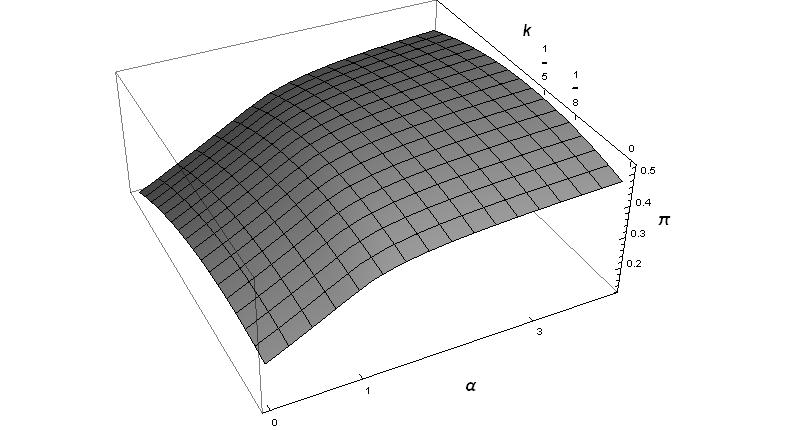
\includegraphics[width=1.0\textwidth]{./figures/Endogenousksimulation0.jpg}
\caption{Simulation of profits with a high cost of piracy }
\flabel{Classic case: Buyers and non-users, }
\label{endk1}
\end{figure}

Similarly we simulate the case where $0<r<\tilde{r}$. Since we now have an additional dimension to represent, we use a 3D contour graph, see figure \ref{endk2}. In this case the $k$ is the optimal k pursued. Notice that once again the equilibrium $k$ is around $\frac{1}{8}$ for low values of product degradation $r$. However, in this scenario, the previous result is reversed, that is, higher piracy pursuit decreases the optimal product improvement. The intuition behind this counterintuitive result is that $r$ and $k$ are substitutes, the firm can use the higher $r$ as an alternative to spending on $k$. In other words, the local effect of an increase in $r$ within $0<r<\tilde{r}$ is to decrease product improvement but once $r=\tilde{r}$, then there is a discontinous jump which depends on the network value which causes an increase in product improvement. 


\begin{figure}[t!] 
\centering
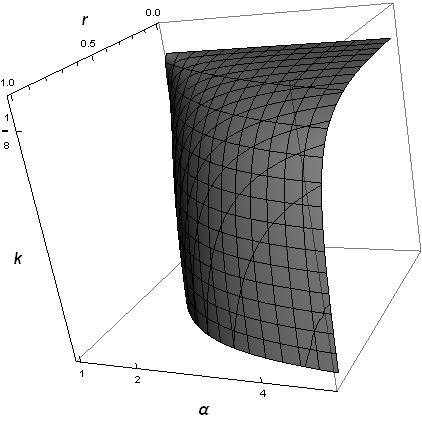
\includegraphics[width=0.5\textwidth]{./figures/Endogenousksimulation.jpg}
\caption{Intermediate cost of piracy case: Contour of the profit function maximized with repspect to the product improvement}
\flabel{Buyers, pirates and non-users}
\label{endk2}
\end{figure}


% In the classic case, where there are no pirates because the cost of piracy is high, the model becomes more complex and has no simple closed form solution for product improvement. If we fix the network value to be equal to base value of the product $\alpha=1+k$, we have that $\tilde{k} = \frac{1}{3 \sqrt{3}} \approx \frac{1}{5}$, numerically this is the highest product improvement that can be pursued, therefore product improvement is maximized when the network value is equal to the base value \footnote{Note that because the cost of product improvement is quadratic, the network value will increase faster than the product improvement, therefore at some point, the equality $\alpha = 1+k$ will hold. If we take the limit of the demand function, $1-\tilde{x}$ with $\alpha$ approaching this parameterization we have that the demand is $\frac{\sqrt{(1+k)(1+k-p)}}{1+k}$. Using this in the profit function, we attain that $p=\frac{2}{27} (9 + \sqrt{3})$ and $k=\frac{1}{3 \sqrt{3}} $ and consequently, profit is, $\pi = \frac{1}{27} \left(1+6 \sqrt{3}\right)$.}.

% In fact even if there is no network value the product improvement pursued is equal the value pursued in the cost-less case,  $\alpha=0 \Rightarrow \tilde{k} = \frac{1}{8}$. Numerically we can also see that as $\alpha$ approaches a large number, $k$ approaches $\frac{1}{9}$
% \footnote{even at $\alpha=100 000 000, k=.1111111$  }. Implying that product improvement peaks when network value is equal to base value. 


% \begin{proposition}
% \label{substitutabilityproposition}
% The network value is substituable with product improvement. 
% \end{proposition}

% \begin{proof}
% See appendix: \ref{substitutabilityproof}
% \end{proof}


% The extra first and second order conditions are given by:

% \begin{equation*}
% \frac{\partial \pi}{\partial k} = \frac{ p(p-r)}{((\alpha-1)
% \sqrt{ 1-r }
% +k)^2} -2k
% \end{equation*}

% \begin{equation*}
% \frac{\partial^2 \pi}{\partial k^2} = -\frac{2 p(p-r)}{((\alpha-1)
% \sqrt{ 1-r }
% +k)^3} -2
% \end{equation*}


% \begin{proposition}
% \label{alphak}
% If $\alpha>1$ then an increase in $\alpha$ can only decrease the pursued product improvement. 
% \end{proposition}

% \begin{proof}
% First we derive with respect to the exogenous variables. Due to the envelope theorem we need only look at the direct effects of the derivative and can ignore indirect effects due to the price. 
% \begin{equation*}
% \frac{\partial \pi }{\partial \alpha} =\frac{\sqrt{1-r}p^* (p^*-r)}{\left((a-1) \sqrt{1-r}+k\right)^2}
% \end{equation*}

% We then proceed to derive with respect to $k$:
% \begin{equation*}
% \frac{\partial^2 \pi }{\partial \alpha k} =
% -\frac{2 \sqrt{1-r} (p^*-r)}{\left((\alpha-1) \sqrt{1-r}+k\right)^3}
% \end{equation*}
% Since this derivative is negative if $\alpha>1$ and $p^*>r$ it implies substitutability between $\alpha$ and k.  
% \end{proof}

% The more intuitive interpretation of proposition \ref{alphak} is simply that the firm will invest to improve the product when the good has a low network value, but as the network value of the good increases, it no longer has need to undertake this investment and since investment is costly, it will just decrease the degree at which it is pursued.

% In the intermediate cost of piracy case, there is once again no closed form solution. Some point estimates, a first and second order approximations are done in the appendix notes(\ref{notes}). However we can deduce how the firm would optimize product improvement with respect to $\alpha$. 

% \begin{corollary}
% Proposition \ref{alphak} implies that the upper bound value of product improvement is $k= \frac{1}{8}$
% \end{corollary}


% To see this corollary we need only note if $\alpha$ was smaller than 1, then the derivative would be positive and therefore the two would be complementary. So the product improvement peaks a $\alpha=1$ and then starts to decrease. In other words, the product improvement pursued when there are no pirates is an upper bound on the intermediate piracy. The firm has a higher incentive to increase the value of its product if pirating is free. 

% \begin{proposition}
% If the network value is large, then further increases in the network value increases the number of buyers. 
% \end{proposition}

% \begin{proof}
% \begin{align*}
% 1 - \hat{x}= 1 - \frac{p-r}{(\alpha - 1) \sqrt{1-r} +k} \\
% = 1 - \frac{k+ (\alpha-1)\sqrt{ 1 -r }-r}{2(\alpha - 1) \sqrt{1-r} +2k} \\
% \frac{\partial (1 - \hat{x})}{\partial \alpha}=  -\frac{ \frac{\partial k}{\partial \alpha}+ \sqrt{ 1 -r }}{2(\alpha - 1) \sqrt{1-r} +2k}+\frac{(k+ (\alpha-1)\sqrt{ 1 -r }-r) (2 \sqrt{1-r}+\frac{\partial k}{\partial \alpha})}{(2(\alpha - 1) \sqrt{1-r} +2k)^2} \\
% =-\frac{\frac{\partial k}{\partial \alpha} \left(\alpha \sqrt{1-r}+k+r-\sqrt{1-r}\right)+2 r\sqrt{1-r} }{4 \left((\alpha-1) \sqrt{1-r}+k\right)^2}
% \end{align*}

% First note that from proposition \ref{alphak} we know that the derivative of k is negative, therefore the whole term is negative if:

% \begin{align*}
% \alpha \sqrt{1-r}+k+r-\sqrt{1-r}<0 \\
% \alpha <1-\frac{k+r}{\sqrt{1-r}}<1 
% \end{align*}

% The above condition never occurs. Because $\alpha>1$ by assumption. 

% We need only check the condition for which the left hand term of the numerator is larger than the right hand term. 
% \begin{align*}
% \alpha>\frac{2 r}{\frac{\partial k}{\partial \alpha}}-\frac{k}{\sqrt{1-r}}-\frac{r}{\sqrt{1-r}}+1 \\
% \end{align*}

% Note that since we know that when $\alpha$ is large, the effect on k approaches 0, this implies that the RHS approaches negative infinity, therefore $\alpha$ increases gradually the proportion of buyers
% \end{proof}

\section{Discussion and Conclusion}
The interpretation so far has been about network goods however a reputation interpretation could work equally well. If we interpret both $\alpha$ and $\beta$ as reputational effects. Both $\alpha$ and $\beta$ can be seen as signalling devices that can only be recognized by the portion of agents who are using. This interpretation may be less intuitive, however it more naturally explains why there may be a differential between the two network values.

The model has been assuming a kind of worse case scenario as to the effect of pirates. Though pirates can be used by the firm to increase its prices, there is no direct revenue mechanism for them. This could easily be imagined in a few cases, for instance, in the digital world a higher use base would allow for indirect profit opportunities. Take a social network as an example, a larger user base allows the network owner to sell advertising slots at a higher price, and the wider the reach the more profitable the enterprise. This kind of mechanism would only strengthen the profits of the firm in the pure piracy case whilist leaving the classic case unaffected. 

Welfare in the model is always decreasing with respect to the cost of piracy. This is simply because the firm mostly does not produce the product since the welfare from an increase in user base is always positive. In the baseline model the product already exists, it only by endogenizing the product improvement that the firm can add value. This does not entail that product degradation should always be zero because profits must be higher than the fixed cost of creating the product. Instead, it should only be noted that the framework presented here actually implies the existence of pareto improving policies. That is, when the network value is high the firm prefers there to be a higher amount of piracy over no piracy at all. 

% In the standard literature, the only source of revenue for a firm is to sell the product. However there are situations, especially in the digital world where having a larger user base also allows for additional indirect profit opportunities. For instance in a social network, a larger user base allows the network owner to sell advertising slots at a higher price, and the wider the reach the more profitable the enterprise. This extra source of revenue is parametrized with the letter $\lambda$. It should be noted that increasing pirates or buyers increase revenue from this source. 

Our model shows that even if the firm has total control of the level of piracy pursuit, it would not necessarily fully utilize this capability. Under the conditions discussed above, the firm often has incentive to not use deterrence to push consumers out of its pool of customers because reducing the number of consumers also decreases the value of the good for those who would buy. The intuition behind this carrot and stick approach is that the price has a single effect whilst piracy pursuit has a double effect. The price effect is less variable because it gives the firm the ability to be more precise in its targeting mechanism. Wile changing the price only works on the consumers who are marginally on the edge of the choice of buying or pirating, changing the degradation level affects all segments at once, resulting in more global network effects. 

Increasing the product degradation affects both the proportion of users buying while also decreasing the user base. The strength of these two effects depends on their valuation of the network value. The decrease in the user base corresponds to the product becoming less popular and the change in buying behavior represents either a consumer who no longer wishes to undertake the risk of pirating or a consumer who no longer wishes to buy the product because it has less value to her.

Though the more traditional way of seeing pirates is as a competitive force, in the model presented here pirates take the role of the path of least resistance. Indeed controlling the pirates to ensure that they are at the right level is a fine art and the if the instrument is too blunt, it may cause more harm than good. The conditions for piracy to be optimal are relatively mild, the bought network value need only reach a certain threshold for it to be worthwhile. Indeed though the model assumed that pursuing pirates is costless, in the real world, there are significant costs both from the point of view of the planner and the firm. The endogenization of these costs would only decrease the threshold $\alpha$ for which the firm would prefer piracy to exist.

One simple policy implication of the model is that pursuing pirates uniformly for all their activities may have welfare reducing effects. An optimal solution would be one where the pursuit of piracy is  heterogeneous to each firm. Much like how firms only sue specific infringers and let others go, the same can be encouraged on the consumer side. From the legal point of view the implication is that piracy could be viewed as a civil or corporate issue and not a criminal one. For broadening the scope of tort law, see \citep{DF96}. 

Still, this approach is limited in that, whilst it is possible for a firm to identify other infringers and selectively sue them, it is likely that the number of pirates is too high to accurately identify. However, if we are to include the cost of identification, this same cost has to be applied on any mechanism that enforces piracy laws. A policy that focuses on enforcement against consumers is likely to have a much higher social cost than one which is enforced on firms in accordance with the actual number of consumers. 

Put in another way, the problem with copyright enforcement is that it is unconditional. That is, unlike patents, where the patent right holder chooses to initiate an action against a patent infringer, presumably following a calculation which leads the patent right holder to the conclusion that such an action is worthwhile. The illegal act of piracy is unconditionally a criminal offense. In other words, regardless of whether the effects of the act aid or harm a copyright owner there is a consistent social cost imposed. 

In practice, firms cannot control the probability of success when initiating an action. In industries where the pirates are many and are highly decentralized, it is quite plausible that neither the government nor the firms can greatly increase their level of piracy pursuit without greatly invading personal data and privacy laws. Realistically, cases involving music or movies are more adapted and fit better into the above developed model. 

It is also important to note that there are firm adaptation which can be used as alternatives to the law. These strategies may be less costly because they can focus on prevention rather than pursuit. In the digital space, these strategies are usually labeled, Digital Rights Management (DRM) strategies. Examples of DRM are idea's such as requiring users to use specific platforms to access the content, monitoring consumption, selling restricted usage copies etc. Such strategies may be complementary or substitutable with piracy enforcement. DRM strategies allow firms to select their own level of piracy pursuit. Piracy often has its own platforms which continously improve their own services. Indeed much of the historic incentive to pirate was due to the superior platform services of piracy software. The new wave of streaming services such as Netflix or Amazon prime represent competition to these piracy services.


A hidden assumption in the model presented above is that all users value socializing with all other users. In the real world, if there are segregation effects, this assumption may not be fully applicable. On the other hand, if we assume that segregation brings together more diverse valuations, such as perhaps a family unit, then this solidifies the conclusions of this model.

Generally, the assumption that utilities are independent is often too readily used. What is termed a "network good" in the industrial organization literature can be interpreted too narrowly. It is not simply digital social networks that have this property. In fact, it is possible to envision most goods as having both an intrinsic value and an extrinsic component. The relative ratio of intrinsic to extrinsic value will likely vary substantially between cultures, space and time. Additionally, the domain in which this is true is likely to extend much farther than what common intuition would entail. For instance, even perishable goods, such as food, are not necessarily exempt from this feedback process, for instance the consumption of cheese or wine is not something that is independent of the surrounding culture. Accordingly, much of what can be deemed "group identity" can be represented within a network good framework. A culture of baguette or chocolate eaters does not represent the same profit opportunities as groups without such culture.

One of the most common arguments against piracy is that it decreases the number of individuals who actually pay the real cost of the product.  However, the implicit assumption in such a line of reasoning is that the number of purchasers and the value of the purchasing, are independent. Based on the model presented here, such a conclusion is drawn too hastily, the effect of increasing the piracy cost may not have the desired effect. As pointed out in \cite{CRP91} this setup raises strange ethical questions. When we have possible parameter values that imply that higher pursuit of pirates may be worse for consumers and producers at public cost. With these factors in mind, it is unclear whether enforcing intellectual property rights passes even the most basic cost benefit analysis.

\newpage
\section{Appendix}
\subsection{Buyers and pirates}
\begin{equation*}
\hat{x} = \frac{p}{\alpha-\beta + k}
\end{equation*}

The upper condition is $\alpha-\beta+k \geq p$. Therefore the price is:

\begin{equation*}
p = \frac{1}{2}\left(
\alpha-\beta+k
\right)
\end{equation*}

Note that these values imply that $\hat{x} = \frac{1}{2}$ regardless of the values of $\beta$ or $\alpha$. Profit is then:
\begin{align*}
\pi &= p(1-\hat{x}) \\
&=  \frac{1}{4}\left(
\alpha-\beta+k
\right)  \\
\end{align*}

Social Surplus and welfare are:
\begin{align*}
\hat{S} &= \int_0^{\hat{x}}x(1+\beta)dx+
\int_{\hat{x}}^{1}\left( x(1+\alpha+k)-p \right)dx \\
&= \frac{1}{8} (\alpha+2 \beta+k+3) \\
\hat{W} &= \frac{3}{8} \left( 1 + \alpha +k
\right)
\end{align*}



\subsection{Proof of proposition \ref{buyersusersprice}} \label{buyersuserspriceproof}

\begin{align*}
\textbf{The demand function in the case of buyers only is given by:} \\
1-\frac{\alpha+k+1-\sqrt{(-\alpha-k-1)^2-4 \alpha p}}{2 \alpha} \\
\frac{\alpha-k-1+\sqrt{(-\alpha-k-1)^2-4 \alpha p}}{2 \alpha}
\\
\textbf{The profit function is then:} 
\\
p*\frac{\alpha-k-1+\sqrt{(-\alpha-k-1)^2-4 \alpha p}}{2 \alpha}
\\
\text{Derivative with respect to p}: \\
\frac{\sqrt{(\alpha+k+1)^2-4 \alpha p}+\alpha-k-1}{2 \alpha}-\frac{p}{\sqrt{(\alpha+k+1)^2-4 \alpha p}} =0
\\
\frac{\sqrt{(\alpha+k+1)^2-4 \alpha p}+\alpha-k-1}{2 \alpha} =\frac{p}{\sqrt{(\alpha+k+1)^2-4 \alpha p}} \\
%%%%%%%%%%%%%%%%%%%%%%%%%%%%%%%%%%%
( \alpha+k+1)^2-4 \alpha p+(\alpha-k-1)\sqrt{(\alpha+k+1)^2-4 \alpha p} = 2 p \alpha \\
( \alpha+k+1)^2+(\alpha-k-1)\sqrt{(\alpha+k+1)^2-4 \alpha p} = 6 p \alpha \\
%%%%%%%%%%%%%%%%%%%%%%%%%%%%%%%%%%%%%
(\alpha-k-1)\sqrt{(\alpha+k+1)^2-4 \alpha p} = 6 p \alpha - ( \alpha+k+1)^2 \\
%%%%%%%%%%%%%%%%%%%%%%%%%%%%%%%%%%%
(\alpha-k-1)^2((\alpha+k+1)^2-4 \alpha p) = (6 p \alpha - ( \alpha+k+1)^2 )^2
%%%%%%%%%%%%%%%%%%%%%%%%%%%%%
% \\
% (\alpha-k-1)^2(\alpha+k+1)^2-(\alpha-k-1)^2 4 \alpha p = 36 p^2 \alpha^2 + ( \alpha+k+1)^4 - 12 p \alpha ( \alpha+k+1)^2 
% \\
% 0 = 36 p^2 \alpha^2  +4 p \alpha((\alpha-k-1)^2-3( \alpha+k+1)^2) + ( \alpha+k+1)^2(( \alpha+k+1)^2-(\alpha-k-1)^2)
% \\
% 0 = 36 p^2 \alpha^2  +4 p \alpha((\alpha-k-1)^2-3( \alpha+k+1)^2) + ( \alpha+k+1)^2(4 \alpha(1+k))
\\
0 = 9 p^2 \alpha  -2 p (\alpha^2 + 4\alpha(1+k)+(1+k)^2) + ( \alpha+k+1)^2 (1+k)
\\
\textbf{This is gives two solutions for p:} \\
\tilde{p} = \frac{(\alpha+k+1)^2+2\alpha(k+1) \pm \sqrt{(1-\alpha+k)^2(\alpha^2+\alpha (k+1)+(k+1)^2)}}{9 \alpha} \\
 = \frac{(\alpha+k+1)^2}{9 \alpha}+\frac{2(1+k)}{9}+\frac{ \pm \sqrt{(1-\alpha+k)^2(\alpha^2+\alpha (k+1)+(k+1)^2)}}{9 \alpha} \\
\end{align*}

If $\alpha$ is large relative to $1+k$, the expression simplifies, we will represent the use of this assumption by $\approx$. 

\begin{align*}
p \approx \frac{\alpha}{9}+\frac{2(1+k)}{9}+\frac{ \pm \sqrt{(\alpha^2+\alpha (k+1))}}{9 } \\
=\frac{\alpha}{9}+\frac{2(1+k)}{9}+\frac{ \pm \sqrt{(\alpha^2+\alpha^2 \frac{(k+1)}{\alpha})}}{9 } \\
=\frac{\alpha}{9}+\frac{2(1+k)}{9}+\frac{ \pm \alpha \sqrt{ \frac{k+1+\alpha}{\alpha}}}{9} \\
=\frac{2\alpha}{9}+\frac{2(1+k)}{9}
\end{align*}


\subsubsection{corollary:}
\label{squareroot}

\begin{align*}
&\sqrt{(\alpha+k+1)^2-4 \alpha p} \\
&\text{Substitute in the approximated price:} \\
&\approx\frac{1}{3} \sqrt{a^2+10 a (k+1)+9 (k+1)^2} \\
&\approx \frac{1}{3} \sqrt{a^2+10  \frac{a^2}{a} (k+1)} \\
&\approx \frac{a}{3} \sqrt{1+ \frac{10}{a} (k+1)} \\
&\approx  \frac{a}{3}
\end{align*}

We can use this expression to represent the proportion of agents who will consume in equilibrium:

\begin{align}
1-\tilde{x} &= 1-\frac{\alpha+k+1-\frac{a}{3}}{2 \alpha} \\
&=\frac{4\alpha-3(1+k)}{6\alpha}
\approx \frac{2}{3}
\end{align}


\subsection{Proof of proposition \ref{piracyvsnotproposition}} \label{piracyvsnot}

We now look at the what the derivative of the profit function turns out to be. First note that in proposition \ref{envelopetheorem} we deduce that the envelope theorem applies. We also use corollary \ref{squareroot} to simplify the square root and proposition to have the simplified price which assume that $\alpha$ is large. 

\begin{align*}
\frac{\partial f}{\partial \alpha} = \frac{\frac{2 (\alpha+k+1)-4 p}{2 \sqrt{(\alpha+k+1)^2-4 \alpha p}}+1}{2
   \alpha}-\frac{\sqrt{(\alpha+k+1)^2-4 \alpha p}+\alpha-k-1}{2 \alpha^2} \\
=\frac{1}{2 \alpha}
\left( 
\frac{2 (\alpha+k+1)-4 p}{2 \sqrt{(\alpha+k+1)^2-4 \alpha p}}+1-\frac{\sqrt{(\alpha+k+1)^2-4 \alpha p}+\alpha-k-1}{ \alpha}
\right) \\
=\frac{1}{2 \alpha}
\left( 
\frac{ (\alpha+k+1)-2 p}{ \sqrt{(\alpha+k+1)^2-4 \alpha p}}-\frac{\sqrt{(\alpha+k+1)^2-4 \alpha p}-k-1}{ \alpha}
\right) \\
=\frac{1}{2 \alpha}
\left( 
\frac{ \alpha (\alpha+k+1)-2 \alpha p}{ \alpha\sqrt{(\alpha+k+1)^2-4 \alpha p}}-\frac{\sqrt{(\alpha+k+1)^2-4 \alpha p}(\sqrt{(\alpha+k+1)^2-4 \alpha p}-k-1)}{ \alpha\sqrt{(\alpha+k+1)^2-4 \alpha p}}
\right) \\
% =\frac{1}{2 \alpha}
% \left( 
% \frac{ \alpha (\alpha+k+1)-2 \alpha p}{ \alpha\sqrt{(\alpha+k+1)^2-4 \alpha p}}-\frac{\sqrt{(\alpha+k+1)^2-4 \alpha p}(\sqrt{(\alpha+k+1)^2-4 \alpha p}-k-1)}{ \alpha\sqrt{(\alpha+k+1)^2-4 \alpha p}}
% \right) \\
% =\frac{1}{2 \alpha^2 \sqrt{(\alpha+k+1)^2-4 \alpha p}}
% \left( 
% \alpha (\alpha+k+1)-2 \alpha p-\sqrt{(\alpha+k+1)^2-4 \alpha p}(\sqrt{(\alpha+k+1)^2-4 \alpha p}+k+1)
% \right) \\
% =\frac{1}{2 \alpha^2 \sqrt{(\alpha+k+1)^2-4 \alpha p}}
% \left( 
% \alpha (\alpha+k+1)-2 \alpha p-(\alpha+k+1)^2+4 \alpha p+(k+1)\sqrt{(\alpha+k+1)^2-4 \alpha p})
% \right) \\
% =\frac{1}{2 \alpha^2 \sqrt{(\alpha+k+1)^2-4 \alpha p}}
% \left( 
% \alpha (\alpha+k+1)-(\alpha+k+1)^2+2 \alpha p+(k+1)\sqrt{(\alpha+k+1)^2-4 \alpha p})
% \right) \\
% =\frac{1}{2 \alpha^2 \sqrt{(\alpha+k+1)^2-4 \alpha p}}
% \left( 
% -(1+k)(\alpha+k+1)^2+2 \alpha p+(k+1)\sqrt{(\alpha+k+1)^2-4 \alpha p})
% \right) \\
=\frac{1}{2 \alpha^2 \sqrt{(\alpha+k+1)^2-4 \alpha p}}
\left( 
2 \alpha p+(k+1)(\sqrt{(\alpha+k+1)^2-4 \alpha p})-(\alpha+k+1)^2)
\right) \\
\textbf{We now assume that $\alpha$ is large relative to k+1 and substitute in the price and square root}
\\
=\frac{3}{2 \alpha^3 }
\left( 
2 \alpha p+(k+1)(\frac{a}{3}-(\alpha+k+1)^2)
\right) \\
=\frac{3}{2 \alpha^3 }
\left( 
2 \alpha (\frac{2\alpha}{9}+\frac{2(1+k)}{9})+(k+1)(\frac{a}{3}-(\alpha+k+1)^2)
\right)
\\
=\frac{3}{2 \alpha^3 }
\left( 
\frac{4\alpha^2}{9}+\frac{4\alpha(1+k)}{9}+(k+1)(\frac{a}{3}-(\alpha+k+1)^2)
\right)\\
=\frac{3}{18 \alpha^3 }
\left( 
4\alpha^2+4\alpha(1+k)+(k+1)(\frac{a}{3}-(\alpha+k+1)^2)
\right)\\
\textbf{Multiply by the price}
\\
p(a)\frac{\partial f}{\partial \alpha} = (\frac{2\alpha}{9}+\frac{2(1+k)}{9})\frac{3}{18 \alpha^3 }
\left( 
4\alpha^2+4\alpha(1+k)+(k+1)(\frac{a}{3}-(\alpha+k+1)^2)
\right)\\
= \frac{\alpha +1+k}{27 \alpha^3 }
\left( 
4\alpha^2+4\alpha(1+k)+(k+1)(\frac{a}{3}-(\alpha+k+1)^2)
\right)
\\
= \frac{\alpha +1+k}{27 \alpha^3 }
\left( 
4\alpha^2+(k+1)(\frac{13a}{3}-(\alpha+k+1)^2)
\right)\\
\end{align*}

\begin{align*}
\text{If alpha is large relative to k+1}\\
= \frac{\alpha}{27 \alpha^3 }
\left( 
4\alpha^2+(k+1)(\frac{13a}{3}-\alpha^2)
\right)
\\
= \frac{1}{27 \alpha^2 }
\left( 
4\alpha^2+(k+1)(\frac{13a}{3}-\alpha^2)
\right) \\
= \frac{1}{27 \alpha^2 }
\left( 
4\alpha^2+(k+1)\frac{\alpha}{3}(13-3 \alpha)
\right)
\\
= \frac{1}{71 \alpha }
\left( 
12\alpha+(k+1)(13-3 \alpha)
\right) \\
\text{If the second term is negative, which occurs after $\alpha$ exceeds 5 we can say}
\\
= \frac{1}{71 \alpha }
\left( 
12\alpha+(k+1)(13-3 \alpha)
\right) < \frac{12}{71 }
\end{align*}
Recall that the slope of the profit function with pirates is $\frac{1}{4}$, therefore profit under piracy increases more than profit without piracy if $\alpha$ is relatively large


% \subsection{Proof of proposition \ref{substitutabilityproposition} }

% \label{substitutabilityproof}

% \begin{proof}
% First note that the cross partial derivative is given by:
% \begin{equation*}
% \frac{\partial^2 \pi}{\partial \alpha k} =
% \frac{p \left(-\frac{\alpha+k+1}{\sqrt{(\alpha+k+1)^2-4 \alpha p}}-\frac{2 \alpha p (\alpha-k-1)}{\left((\alpha+k+1)^2-4 \alpha p\right)^{3/2}}+1\right)}{2 \alpha^2} 
% \end{equation*}

% To check the sign we need only see that the two first terms inside the parenthesis are decreasing in $\alpha$. 
% \begin{align*}
% &= \left(-\frac{\alpha+k+1}{\sqrt{(\alpha+k+1)^2-4 \alpha p}}-\frac{2 \alpha p (\alpha-k-1)}{\left((\alpha+k+1)^2-4 \alpha p\right)^{3/2}}+1\right)&& \\
% %%%%%%%%%%%%%%%%%%%%%%%%%%%%%%%%%
% &= 1- \frac{2 \alpha p (\alpha-k-1)+((\alpha+k+1)^2-4 \alpha p)(1+k+\alpha)}{\left((\alpha+k+1)^2-4 \alpha p\right)^{3/2}}& \\
% %%%%%%%%%%%%%%%%%%%%%%%%%%%%%%%%%
% &= \frac{\left((\alpha+k+1)^2-4 \alpha p\right)^{3/2}-2 \alpha p (\alpha-k-1)-((\alpha+k+1)^2-4 \alpha p)(1+k+\alpha)}{\left((\alpha+k+1)^2-4 \alpha p\right)^{3/2}}& \\
% %%%%%%%%%%%%%%%%%%%%%%%%%%%%%%%%%
% &=\frac{\left((\alpha+k+1)^2-4 \alpha p\right)^{3/2}+2 \alpha p (\alpha-3(k+1))-((\alpha+k+1)^3}{\left((\alpha+k+1)^2-4 \alpha p\right)^{3/2}} &
% \end{align*}*

% Note that if $\alpha=0$ then the cross partial is 0. Then note that in the last expression, the last term is always larger than the first term when $k>0,\alpha>0, p>0$. Then note that the second term is negative whenever $\alpha<3$ and if $\alpha>3$ then the cube route effect of the last term dominates.  
% \end{proof}

\subsection{Proof of proposition \ref{tdemand}}

\label{tdemandp}

We first begin with the condition which renders an agents indifferent between pirating and not using to solve for the valuation $x$ of the indifferent pirate. 


\begin{align*}
x(1+\beta(1-F(x)))-r=0 \\
x(1+\beta(1-x))=0 \\
x+x\beta-\beta x^2-r=0 \\
x^2-x\frac{(1+\beta)}{\beta} +\frac{r}{\beta} = 0 \\
\check{x} = \frac{(1+\beta)}{2 \beta}
\pm
\frac{ \sqrt{ \left(\frac{(1+\beta)}{\beta}\right)^2 -4\frac{r}{\beta} } }{2} \\
\check{x} = \frac{(1+\beta)}{2 \beta}
\pm
\frac{ \sqrt{ \left(1+\beta\right)^2 -4r\beta } }{2 \beta} \\
\end{align*}



\begin{equation*}
\check{x} = 1
\pm \sqrt{ 1 -r }
\end{equation*}

If $\check{x}>1$ is verified this implies that no users will be pirating since all users prefer not to pirate. Therefore only the negative solution can be used.  With the indifferent user, we need only take the difference $1-\check{x}$ to know the proportion of agents who are users. This proportion is simply:

\begin{align*}
1-\check{x}=\sqrt{ 1 -r }
\end{align*}

We note that the proportion of agents who are users is entirely exogenous to the firm. What is endogenous to the firm is the proportion of agents who are buyers. The proportion of agents who are buyers, ceteris parabus, depends on the proportion who are pirates. The consumer who is indifferent between purchasing and pirating can similarly be found by equating the two options. Which gives the following value:

\begin{align*}
x(1+\beta(1-F(x)))-r=x(1+\alpha(1-F(x)))-p \\
\Rightarrow \hat{x}=\frac{p-r}{(\alpha-1)\sqrt{ 1 -r }+k} \\
\end{align*}

Where the last step occurs because $1-F(x)=1-\check{x}$. Recall that $\hat{x} \geq \check{x}$ from the preliminary section. The demand function for buying can then simply be written as:

\begin{align*}
D(\hat{x})=1-\hat{x}=1-\frac{ (p-r)}{k + (\alpha-1) \sqrt{ 1 -r }} \\
%%%%%%%%%%%%%%%%%%%%%%%%%%%%%%%%
\frac{\partial D(\hat{x})}{\partial p} =
-\frac{ 1}{k + (\alpha-1) \sqrt{ 1 -r }} \\
%%%%%%%%%%%%%%%%%%%%%%%%%%%%%%%%%
\frac{\partial D(\hat{x})}{\partial k} =
\frac{ (p-r) }{(k+
 (\alpha-1)\sqrt{ 1 - r }
)^2} 
%%%%%%%%%%%%%%%%%%%%%%%%%%%%%%%%%
%%%%%%%%%%%%%%%%%%%%%
\end{align*}

% This condition must satisfy that the higher indifferent agent must have a lower valuation, $x$ than the highest valuation user, $\hat{x} \leq 1$. This constraint can be used to give us an upper bound on the price the firm can charge. We call this condition 1, $C_1$

% \begin{align*}
% \hat{x} \leq 1 \\
% \frac{p-r}{(\alpha-1)\sqrt{ 1 -r }+k} \leq 1
% \\
% p \leq (\alpha-1)\sqrt{ 1 -r }+k+r \\
% \text{or we can get an upper bound on k} \\
% p -(\alpha-1)\sqrt{ 1 -r } -r\leq k \\
% \text{similarly we can use the lower bound:} \\
% \hat{x} \geq 0 \\
% \frac{p-r}{(\alpha-1)\sqrt{ 1 -r }+k}  \geq 0 \\
% p \geq r
% \end{align*}

% We similarly recall that the indifferent consumer between buying and pirating must be higher than the indifferent consumer between pirating and not buying, $\hat{x}>\check{x}$. We can use this condition to get a further condition.  We call this the second condition $C_2$
% \begin{align*}
% C_2 = \frac{p-r}{(\alpha-1)\sqrt{ 1 -r }+k} -\sqrt{ 1 -r } \geq 0
% \\
% \frac{p-r}{(\alpha-1)\sqrt{ 1 -r }+k} 
% \geq
% \sqrt{ 1 -r } \\
% p-r
% \geq \sqrt{ 1 -r }((\alpha-1)\sqrt{ 1 -r }+k) \\
% p-r
% \geq (\alpha-1)( 1 -r )+k\sqrt{ 1 -r } \\
% p
% \geq \alpha -1+r(2-\alpha)+k\sqrt{ 1 -r }
% \end{align*}

% We can compare this constraint to the previous one to see that this one is stricter:

% \begin{align*}
% -1+r(2-\alpha)+k\sqrt{ 1 -r } \geq r \\
% \Rightarrow
% k\sqrt{ 1 -r } + (1 -r)(\alpha-1) \geq 0
% \end{align*}








\section{Endogenous k}


\subsection{case where $r=0$}

\begin{proposition}
If $r=0$, the firm will choose $(p,k)=(\frac{1}{16c}+\frac{\alpha-\beta}{2},\frac{1}{8c})$ $\check{x}=0$ and $\hat{x}=1/2$ and $\pi= \frac{1}{4}(\alpha-\beta)+\frac{1}{64c}$.
\end{proposition}

\begin{proof}


As in the exogenous case we solve for the indifference condition:

\begin{align*}
\hat{x}(1+\alpha+k)=\hat{x}(1+\beta) \\
\Rightarrow \hat{x} = \frac{p}{\alpha - \beta +k}
\end{align*}


Now, the profit function is

\begin{equation*}
\tilde{\pi} = p\left(1-\frac{p}{\alpha - \beta +k}\right)-c k^2
\end{equation*}

The two first order conditions, relatives to $p$ and $k$, for the profit maximization are:

\begin{align*}
\frac{\partial \tilde{\pi}}{\partial p}= 1-\frac{2p}{\alpha - \beta +k}\\
\frac{\partial \tilde{\pi}}{\partial k}=  \frac{p^2}{(\alpha-\beta+k)^2}-2ck 
\end{align*} 

\begin{equation*}
p = \frac{\alpha-\beta-k}{2}
\end{equation*}

and 

\begin{equation*}
2ck = \frac{p^2}{(\alpha-\beta+k)^2}
\end{equation*}

This gives $k^*=\frac{1}{8c}$,  and $p^*=\frac{\alpha-\beta}{2}+\frac{1}{16c}$ and $\pi=\frac{1}{4}(\alpha-\beta)+\frac{1}{64c} $ if we put these values in the profit equation. 

\end{proof}

\begin{observation}
The product improvement chosen by the firm does not depend on network values, $\beta$ and $\alpha$
\end{observation}


\subsection{Intermediate r}
$0<r<\tilde{r}$

We need to also verify that the profit function satisfies the first and second order conditions with respect to the price level.

\begin{align*}
\pi = p\left(1-\hat{x}\right) - k^2 \\
%%%%%%%%%%%%%%%%%%%%%
=p\left(1-\frac{ (p-r)}{(\alpha-1)
\sqrt{ 1-r }
+k} \right) -k^2
\\
%%%%%%%%%%%%%%%%%%%%%
\frac{\partial \pi }{\partial p} = 1-\frac{ (2p-r)}{
k+ (\alpha-1)\sqrt{ 1 -r }} \\
%%%%%%%%%%%%%%%%%%%%%
\frac{\partial^2 \pi }{\partial p^2}
= -\frac{ 2}{
k+ (\alpha-1)\sqrt{ 1 -r }} \\
%%%%%%%%%%%%%%%%%%%%%
%%%%%%%%%%%%%%%%%%%%%
%%%%%%%%%%%%%%%%%%%%%
\frac{\partial \pi}{\partial k} = \frac{ p(p-r)}{((\alpha-1)
\sqrt{ 1-r }
+k)^2} -2k
\\
%%%%%%%%%%%%%%%%%%%%%
\frac{\partial^2 \pi}{\partial k^2} = -\frac{2 p(p-r)}{((\alpha-1)
\sqrt{ 1-r }
+k)^3} -2 
\end{align*}

\subsection{Some values for k}

We now set $ (\alpha-1)\sqrt{ 1 -r }=w$ and proceed to solve for $k$ using the second FOC.  

\begin{align*}
\frac{\partial \pi}{\partial k} = \frac{ p(p-r)}{(w
+k)^2} -2k \\
2k= \frac{ p(p-r)}{(w
+k)^2} \\
2k(w+k)^2=p(p-r) \\
\text{We now substitute the price into the this: } \\
2k(w+k)^2=\frac{k+ w+r}{2} \left(\frac{k+ w+r}{2}-r \right) \\
2k(w+k)^2=\frac{k+ w+r}{2} \left(\frac{k+ w-r}{2} \right) \\
8k(w+k)^2= \left( k+ w+r \right) \left(k+ w-r\right) \\
\text{If we assume that $w=r$} \\
\Rightarrow 
k = \frac{1}{16} \left(1\pm \sqrt{32 r+1}\right) - r\\
\text{Only the positive solution yields positive values} \\
= \frac{1}{16} \left(1\pm \sqrt{32 r+1}\right) - r \\
\text{This function is maximized at $k=\frac{1}{8}$} \\
\text{We now take a limit case as $\alpha$ increases:} \\
8k(w+k)^2= \left( w+ k \right)^2 \\
k = \frac{1}{8} \\
\text{Similarly if:} \\
\alpha=1=\beta \\
\Rightarrow w = 0 \\
\Rightarrow k = \frac{1}{8} 
\end{align*}

\subsection{Notes} \label{notes}

\subsubsection{Why the envelope theorem applies} \label{envelopetheorem}


For notational simplicity we represent the demand function which is a function of $\alpha, p, k$ as $l(a, k(a),p(a))$.  

\begin{align*}
\pi(a, p(a),k(a))= p(a) l(a, k(a),p(a))-k(a)^2 \\
%%%%%%%%%%%%%%%%%%%%%%%%%%%%%%%%
\frac{ \partial \pi(a, p(a),k(a))}{\partial \alpha}= \frac{\partial p(a) }{\partial a } \left(
l(a, k(a),p(a)) \right)
+ p(a)\left( \frac{\partial l}{\partial a}
+\frac{\partial l}{\partial k(a)}\frac{\partial k(a)}{\partial a}
+\frac{\partial l}{\partial p(a)}\frac{\partial p(a)}{\partial a}
\right)
- 2 k(a) \frac{\partial k(a)}{\partial a}
\\ 
%%%%%%%%%%%%%%%%%%%%%%%%%%%
= \frac{\partial p(a) }{\partial a } \left(
l(a, k(a),p(a)) +p(a) \frac{\partial l}{\partial p(a)} \right)
+ p(a) \frac{\partial l}{\partial a}
+\frac{\partial k(a)}{\partial a}\left( p(a)\frac{\partial l}{\partial k(a)}-2 k(a)
 \right) \\
FOCS: 
\\
\frac{\partial \pi(a, p(a),k(a))}{\partial p(a)}=l(a, k(a),p(a))+p(a) \frac{\partial l}{\partial p(a)}=0 
\\
\frac{\partial \pi(a, p(a),k(a))}{\partial k(a)}=p(a) \frac{\partial l}{\partial k(a)} -2 k(a)=0
\\
\textbf{applying the FOC's we can simplify to}
\\
\frac{ \partial \pi(a, p(a),k(a))}{\partial \alpha}= 
p(a) \frac{\partial l}{\partial a} \\
\end{align*}

Therefore we can deduce the effects of $\alpha$ by simply taking the direct derivative of the profit function. The argument is equivalent for $r$.

\subsubsection{Regularly varying functions}

\begin{definition}
A regularly varyng function $L: (0,+ \infty) \rightarrow (0,+ \infty)$ has the following property:
\begin{equation}
lim_{x \rightarrow \infty} \frac{L(t x)}{L(x)} = g(t)
\end{equation}
\end{definition}

It is known that in regular varying functions, $g(t)$ take the following form\citep{bojanic1963slowly}:
\begin{equation}
g(t)=t^i
\end{equation}

If $g(t)= t$ this implies that the function is eventually linear. 

\begin{align}
L(x)-L(a x) = L(x) - f(a)L(x) = L(x)(1-f(a)) \\
L(y)-L(b y) = L(y) - f(b)L(y) = L(y)(1-f(b)) \\
\text{Linearity  implies:}
x-ax = y-yb \\
\rightarrow y = x \frac{(1-a)}{(1-b)} \\
\rightarrow L\left(x \frac{1-a}{1-b}\right)[1-f(b)] \\
\rightarrow f\left( \frac{1-a}{1-b}\right)L(x)[1-f(b)] \\
\text{L is linear in x if} \\
L(x)f\left(\frac{1-a}{1-b}\right)(1-f(b)) = L(x)(1-f(a)) \\
f\left(\frac{1-a}{1-b} \right) = \frac{1-f(a)}{1-f(b)} \\
\left(\frac{1-a}{1-b} \right)^i = \frac{1-a^i}{1-b^i} 
\end{align}

Which is satisfied because $g(t)=t$ implies $i=1$

\subsubsection{Welfare}

Welfare is just the sum of the social surplus and the profit.

\begin{align*}
W_{bn} = \int^{\tilde{x}}_0 \left(x(1+\alpha(1-\tilde{x})+\tilde{k})-\tilde{p} \right) dx + \tilde{\pi}  \\
W_{bp} = \int^{\hat{x}}_0 x(1+\beta) dx +\int^{1}_{\hat{x}} \left(x(1+\alpha+\hat{k}) - \hat{p} \right) dx + \hat{\pi} \\
W_{bpn} =
\int^{\hat{x}}_{\check{x}} \left(x(1+\beta(1-\check{x}))-r \right)dx +\int^{1}_{\hat{x}} \left(x(1+\alpha(1-\check{x})+\check{k}) - \check{p} \right) dx + \check{\pi}
\end{align*}

\subsubsection{First and second order approximations of endogenous k}

\begin{align*}
\text{If we don't take the limit case then this is:} \\
8k(w+k)^2= \left( w+k \right)^2 -r^2 \\
(w+k)^2(8k-1)=-r^2 \\
\text{If we take a first order approximation:} \\
f(k)= (w+k)^2(8k-1)+r^2 
\\
\approx f(t)+f'(t)(k-t) \\
=(8 t-1) (t+w)^2+r^2 
+(8 (t+w)^2+2 (8 t-1) (t+w))(k-t) \\
\Rightarrow k = \frac{2 t+w^2+2 w-15 t^2-14 t w-r^2}{8 (t+w)^2}
\\
\text{If we approximate around $t=\frac{1}{8}$} \\
k = \frac{(8 w+1)^2-64 r^2}{8 (8 w+1)^2} 
\\
\text{If we approximate around $t=0$} \\
k= \frac{w (w+2)-r^2}{8 w^2}
\\
\text{So k is decreasing with r} \\
\end{align*}

\begin{align*}
\text{A second order approximation of the function:} \\ 
f(k)= (w+k)^2(8k-1)+r^2 \\
\approx f(t)+f'(t)(k-t)+\frac{f''(\alpha)}{2}(k-t)^2 \\
= (8 t-1) (t+w)^2+r^2 
+(8 (t+w)^2+2 (8 t-1) (t+w))(k-t) \\
+\frac{32 (t+w)+2 (8 t-1)}{2}(k-t)^2 \\
= (8 t-1) (t+w)^2+r^2 
+(8 (t+w)^2+2 (8 t-1) (t+w))(k-t) \\
+(16 (t+w)+ (8 t-1))(k-t)^2 
\end{align*}



%\begin{equation*}
%k = \frac{\pm \sqrt{\left(2 t-40 t^2-16 %t w+8 w^2\right)^2-4 (24 t+16 w-1) %\left(r^2+24 t^3+16 t^2 w+14 t^2+14 t %w-2 t-w^2-2 w\right)}+40 t^2+16 t w-2 %t-8 w^2}{2(24 t+16 w-1)} 
%\end{equation*}
We solve for k around 0: 

\begin{align*}
k = \frac{\pm \sqrt{\left(8 w^2\right)^2-4 (16 w-1) \left(r^2-w^2-2 w\right)}-8 w^2}{2(16 w-1)} \\
=\frac{\pm 2 \sqrt{16 w^4- (16 w-1) \left(r^2-w^2-2 w\right)}-8 w^2}{2(16 w-1)} \\
=\frac{\pm \sqrt{16 w^4- (16 w-1) \left(r^2-w^2-2 w\right)}-4 w^2}{16 w-1} \\
\text{only the positive solution gives a positive answer:} \\
= \frac{ \sqrt{16 w^4- (16 w-1) \left(r^2-w^2-2 w\right)}-4 w^2}{16 w-1}
\end{align*}








\end{document}
